%%%%%%%%%%%%%%%%%%%%%%%%%%%%%%%%%%%%%%%%%
% Masters/Doctoral Thesis 
% LaTeX Template
% Version 2.5 (27/8/17)
%
% This template was downloaded from:
% http://www.LaTeXTemplates.com
%
% Version 2.x major modifications by:
% Vel (vel@latextemplates.com)
%
% This template is based on a template by:
% Steve Gunn (http://users.ecs.soton.ac.uk/srg/softwaretools/document/templates/)
% Sunil Patel (http://www.sunilpatel.co.uk/thesis-template/)
%
% Template license:
% CC BY-NC-SA 3.0 (http://creativecommons.org/licenses/by-nc-sa/3.0/)
%
%%%%%%%%%%%%%%%%%%%%%%%%%%%%%%%%%%%%%%%%%

%----------------------------------------------------------------------------------------
%	PACKAGES AND OTHER DOCUMENT CONFIGURATIONS
%----------------------------------------------------------------------------------------

\documentclass[
11pt, % The default document font size, options: 10pt, 11pt, 12pt
%oneside, % Two side (alternating margins) for binding by default, uncomment to switch to one side
ngerman,
english, % ngerman for German
singlespacing, % Single line spacing, alternatives: onehalfspacing or doublespacing
%draft, % Uncomment to enable draft mode (no pictures, no links, overfull hboxes indicated)
%nolistspacing, % If the document is onehalfspacing or doublespacing, uncomment this to set spacing in lists to single
%liststotoc, % Uncomment to add the list of figures/tables/etc to the table of contents
%toctotoc, % Uncomment to add the main table of contents to the table of contents
%parskip, % Uncomment to add space between paragraphs
%nohyperref, % Uncomment to not load the hyperref package
headsepline, % Uncomment to get a line under the header
%chapterinoneline, % Uncomment to place the chapter title next to the number on one line
%consistentlayout, % Uncomment to change the layout of the declaration, abstract and acknowledgements pages to match the default layout
]{MastersDoctoralThesis} % The class file specifying the document structure

\usepackage[utf8]{inputenc} % Required for inputting international characters
\usepackage[T1]{fontenc} % Output font encoding for international characters

\usepackage{mhchem} % chemical reactions 

%\usepackage{mathpazo} % Use the Palatino font by default
\usepackage{lmodern} % Use the Latin Modern font by default

%\usepackage[backend=bibtex,style=authoryear,natbib=true]{biblatex} % Use the bibtex backend with the authoryear citation style (which resembles APA)
\usepackage[backend=bibtex,style=numeric-comp,natbib=true,sorting=none]{biblatex} % Use the bibtex backend with the numeric-comp citation style (which resembles APA), sorting=none is for sorting reference automatically.
%\usepackage[square,numbers]{natbib}

\addbibresource{example.bib} % The filename of the bibliography

\usepackage[autostyle=true]{csquotes} % Required to generate language-dependent quotes in the bibliography
%====================
% To strike out sth
\usepackage{calc}
\newsavebox\CBox
\newcommand\hcancel[2][0.5pt]{%
  \ifmmode\sbox\CBox{$#2$}\else\sbox\CBox{#2}\fi%
  \makebox[0pt][l]{\usebox\CBox}%  
  \rule[0.5\ht\CBox-#1/2]{\wd\CBox}{#1}}
% Example: \hcancel[2pt]{xxx}
%====================
\usepackage[normalem]{ulem}
%\usepackage{amsmath} 
\newcommand{\stkout}[1]{\ifmmode\text{\sout{\ensuremath{#1}}}\else\sout{#1}\fi}
%====================

% add from other template
\usepackage{amsmath, amssymb}
%\usepackage{graphics} 
\usepackage{wrapfig,lipsum,booktabs}
\usepackage{setspace}
\usepackage{enumerate}
\usepackage[]{subfig}
%\usepackage{fancyhdr}
\usepackage{eucal}
\usepackage[below]{placeins}
%\usepackage[english]{babel}
%\usepackage[usenames, dvipsnames]{color}
%\usepackage[perpage]{footmisc}
%\usepackage{multirow}
%\usepackage{ifthen}
%\usepackage[square,sort,comma,numbers]{natbib} % Gang
\usepackage{mathrsfs} % Curlicue characters %Gang
%\usepackage{dcolumn}% Align table columns on decimal point %Gang
\usepackage{bm}% bold math %Gang
\usepackage{sidecap} %Gang
% Nomenclature
\usepackage{nomencl}
\usepackage{graphicx} % Include figure files
\usepackage{epstopdf} % PDFLATEX is not able to handle EPS graphic files, but converters epstopdf will help. The best way is to include epstopdf, which must follow the graphicx package
\usepackage{float}  %introduces a placement option H enforcing the placement exactly at that point.
\usepackage{placeins} %provides the command \FloatBarrier to limit the floating of figures or tables. You could place such a barrier before and after a listing.
\usepackage{xcolor}
\usepackage{color}
\usepackage{soul}
\usepackage{xspace} %In order to have space after "\newcommands" 
\usepackage{listings}  %use for listing source codes
%\usepackage[all,cmtip]{xy}  %xypic
\lstset{ 
    language=python, % choose the language of the code
    basicstyle=\fontfamily{pcr}\selectfont\footnotesize\color{black},
    %keywordstyle=\color{red}\bfseries, % style for keywords
    keywordstyle=\color{black}\bfseries, % style for keywords % Gang
    numbers=none, % where to put the line-numbers
    numberstyle=\tiny, % the size of the fonts that are used for the line-numbers     
    backgroundcolor=\color{white}, % we can also choose: darkgray
    showspaces=false, % show spaces adding particular underscores
    showstringspaces=false, % underline spaces within strings
    showtabs=false, % show tabs within strings adding particular underscores
    frame=single, % adds a frame around the code
    tabsize=2, % sets default tabsize to 2 spaces
    rulesepcolor=\color{gray},
    rulecolor=\color{black},
    captionpos=b, % sets the caption-position to bottom
    breaklines=true, % sets automatic line breaking
    breakatwhitespace=false, 
}
%\usepackage[toc,page]{appendix} %For adding appendices
\usepackage{pgfplots} % a plotting package in latex
\usepackage[export]{adjustbox}[2011/08/13]

%=================================================
%(Re-)New commands
%=================================================
%\renewcommand{\nomname}{List of Symbols and Abbreviations}
\newcommand{\etal}{\textit{et al.}}
\newcommand{\abinitio}{\textit{ab initio}\xspace}
\newcommand{\Li}{Li$^{+}$\xspace}
\newcommand{\Na}{Na$^{+}$\xspace}
\newcommand{\K}{K$^{+}$\xspace}
\newcommand{\Cl}{Cl$^{-}$\xspace}
\newcommand{\Br}{Br$^{-}$\xspace}
\newcommand{\I}{I$^{-}$\xspace}
\newcommand{\li}{Li$^{+}$}
\newcommand{\na}{Na$^{+}$}
\newcommand{\pot}{K$^{+}$}
\newcommand{\cl}{Cl$^{-}$}
\newcommand{\br}{Br$^{-}$}
\newcommand{\Iodine}{I$^{-}$}
\newcommand{\COO}{COO$^{-}$\xspace}
\newcommand{\sfg}{Sum Frequency Generation\xspace}
%\newcommand{\cm}{cm$^{-1}$~\xspace}
\newcommand{\cm}{cm$^{-1}$\thinspace}
\newcommand{\centimeter}{cm$^{-1}$}
\newcommand{\nm}{nm$^{-2}$\xspace}
\newcommand{\z}{\textit{z}-axis\xspace}
\newcommand{\water}{H$_2$O\xspace}
\newcommand{\wat}{H$_2$O}
\newcommand{\NVT}{\textit{NVT}\xspace}
\newcommand{\T}{\textit{T}\xspace}
\newcommand{\nitrate}{NO$_3^-$\xspace}
\newcommand{\nit}{NO$_3^-$}
\newcommand{\LiN}{LiNO$_3$\xspace}
\newcommand{\X}{$x$\xspace}
\newcommand{\Y}{$y$\xspace}
\newcommand{\Z}{$z$\xspace}
\newcommand*{\tran}{^{\mkern-1.5mu\mathsf{T}}}

%
\newcommand{\rt}{$t_\text{t}$\xspace}

%
\newcommand{\hbo}{$h(t)$\xspace}
\newcommand{\hbos}{$h^\text{(s)}(t)$\xspace}
\newcommand{\CHB}{$c(t)$\xspace}
\newcommand{\SHB}{$s(t)$\xspace}
\newcommand{\CSHB}{$c^\text{(s)}(t)$\xspace}
\newcommand{\SSHB}{$s^\text{(s)}(t)$\xspace}
\newcommand{\LiFourW}{[Li$\cdot$(H$_2$O)$_4$]$^+$}
\newcommand{\rI}{$r_{\text{I}^-}$}
\newcommand{\rcation}{$r_\text{cation}$}
%Renew the \AA command in order to have a space when we want
\let\oldAA\AA
\renewcommand{\AA}{\oldAA\xspace}
\newcommand{\A}{\oldAA}
%=================================================

%----------------------------------------------------------------------------------------
%	MARGIN SETTINGS
%----------------------------------------------------------------------------------------

\geometry{
	paper=a4paper, % Change to letterpaper for US letter
	inner=2.5cm, % Inner margin
	outer=3.8cm, % Outer margin
	bindingoffset=.5cm, % Binding offset
	top=1.5cm, % Top margin
	bottom=1.5cm, % Bottom margin
	%showframe, % Uncomment to show how the type block is set on the page
}

%----------------------------------------------------------------------------------------
%	THESIS INFORMATION
%----------------------------------------------------------------------------------------

\thesistitle{Structure, Dynamics and Vibrational Spectroscopy of Interfacial 
Alkali Nitrate Aqueous Solutions from \abinitio Molecular Dynamics} % Your thesis title, this is used in the title and abstract, print it elsewhere with \ttitle
\thesistitleG{Struktur-, Dynamik- und Schwingungsspektroskopie von Alkaligrenzflächen
Wässrige Nitratlösungen von \abinitio Molecular Dynamics} % Your thesis title, this is used in the title and abstract, print it elsewhere with \ttitle
\supervisor{Apl. Prof. Dr. Marialore \textsc{Sulpizi}} % Your supervisor's name, this is used in the title page, print it elsewhere with \supname
\examiner{Apl. Prof. Dr. Marialore Sulpizi, Prof. Dr. Wittig, Prof. Dr. Palberg, Prof. Dr. Spiesberger} % Your examiner's name, this is not currently used anywhere in the template, print it elsewhere with \examname
\degree{Doctor of Philosophy} % Your degree name, this is used in the title page and abstract, print it elsewhere with \degreename
\degreeG{Doktor der Philosophie} % Your degree name, this is used in the title page and abstract, print it elsewhere with \degreename
\author{Gang \textsc{Huang}} % Your name, this is used in the title page and abstract, print it elsewhere with \authorname
\addresses{} % Your address, this is not currently used anywhere in the template, print it elsewhere with \addressname

\subject{Statistical Physics and Soft Matter} % Your subject area, this is not currently used anywhere in the template, print it elsewhere with \subjectname
\subjectG{Statistische Physik und weiche Materie} % Your subject area, this is not currently used anywhere in the template, print it elsewhere with \subjectname
\keywords{sum-frequency generation, hydrogen bond dynamics, water/vapor interfaces} % Keywords for your thesis, this is not currently used anywhere in the template, print it elsewhere with \keywordnames
\keywordsG{Summenfrequenzerzeugung, Wasserstoffbrückendynamik, Wasser/Dampf-Grenzflächen} % Keywords for your thesis, this is not currently used anywhere in the template, print it elsewhere with \keywordnames
\university{\href{https://www.uni-mainz.de}{Johannes Gutenberg University Mainz}} % Your university's name and URL, this is used in the title page and abstract, print it elsewhere with \univname
\universityG{\href{https://www.uni-mainz.de}{Johannes Gutenberg Universit\"at Mainz}} % Your university's name and URL, this is used in the title page and abstract, print it elsewhere with \univname
\department{\href{https://www.iph.uni-mainz.de}{Institute for Physics }} % Your department's name and URL, this is used in the title page and abstract, print it elsewhere with \deptname
\departmentG{\href{https://www.iph.uni-mainz.de}{Institut für Physik}} % Your department's name and URL, this is used in the title page and abstract, print it elsewhere with \deptname
\group{\href{https://www.komet1.physik.uni-mainz.de}{Condensed Matter Theory Group}} % Your research group's name and URL, this is used in the title page, print it elsewhere with \groupname
\groupG{\href{https://www.komet1.physik.uni-mainz.de}{Gruppe zur Theorie der kondensierten Materie}} % Your research group's name and URL, this is used in the title page, print it elsewhere with \groupname
\faculty{\href{https://www.komet1.physik.uni-mainz.de}{Condensed Matter Theory}} % Your faculty's name and URL, this is used in the title page and abstract, print it elsewhere with \facname
\facultyG{\href{https://www.komet1.physik.uni-mainz.de}{Theorie der kondensierten Materie}} % Your faculty's name and URL, this is used in the title page and abstract, print it elsewhere with \facname

\AtBeginDocument{
\hypersetup{pdftitle=\ttitle} % Set the PDF's title to your title
\hypersetup{pdfauthor=\authorname} % Set the PDF's author to your name
\hypersetup{pdfkeywords=\keywordnames} % Set the PDF's keywords to your keywords
}

\DeclareUnicodeCharacter{2212}{-} % Minus sign (by Gang Huang)


\begin{document}

\frontmatter % Use roman page numbering style (i, ii, iii, iv...) for the pre-content pages

\pagestyle{plain} % Default to the plain heading style until the thesis style is called for the body content

%----------------------------------------------------------------------------------------
%	TITLE PAGE
%----------------------------------------------------------------------------------------

\begin{titlepage}
\begin{center}

\vspace*{.06\textheight}
{\scshape\LARGE \univname\par}\vspace{1.5cm} % University name
\textsc{\Large Doctoral Thesis}\\[0.5cm] % Thesis type

\HRule \\[0.4cm] % Horizontal line
{\huge \bfseries \ttitle\par}\vspace{0.4cm} % Thesis title
\HRule \\[1.5cm] % Horizontal line
 
\begin{minipage}[t]{0.4\textwidth}
\begin{flushleft} \large
\emph{Author:}\\
\href{http://www.johnsmith.com}{\authorname} % Author name - remove the \href bracket to remove the link
\end{flushleft}
\end{minipage}
\begin{minipage}[t]{0.4\textwidth}
\begin{flushright} \large
\emph{Supervisor:} \\
\href{https://www.staff.uni-mainz.de/sulpizi}{\supname} % Supervisor name - remove the \href bracket to remove the link  
\end{flushright}
\end{minipage}\\[3cm]
 
\vfill

\large \textit{A thesis submitted in fulfillment of the requirements\\ for the degree of \degreename}\\[0.3cm] % University requirement text
\textit{in the}\\[0.4cm]
\groupname\\\deptname\\[2cm] % Research group name and department name
 
\vfill

{\large \today}\\[4cm] % Date
%\includegraphics{Logo} % University/department logo - uncomment to place it
 
\vfill
\end{center}
\end{titlepage}

%----------------------------------------------------------------------------------------
%	DECLARATION PAGE
%----------------------------------------------------------------------------------------

\begin{declaration}
\addchaptertocentry{\authorshipname} % Add the declaration to the table of contents
\noindent I, \authorname, declare that this thesis titled, \enquote{\ttitle} and the work presented in it are my own. I confirm that:

\begin{itemize} 
\item This work was done wholly or mainly while in candidature for a research degree at this University.
\item Where any part of this thesis has previously been submitted for a degree or any other qualification at this University or any other institution, this has been clearly stated.
\item Where I have consulted the published work of others, this is always clearly attributed.
\item Where I have quoted from the work of others, the source is always given. With the exception of such quotations, this thesis is entirely my own work.
\item I have acknowledged all main sources of help.
\item Where the thesis is based on work done by myself jointly with others, I have made clear exactly what was done by others and what I have contributed myself.\\
\end{itemize}
 
\noindent Signed:\\
\rule[0.5em]{25em}{0.5pt} % This prints a line for the signature
 
\noindent Date:\\
\rule[0.5em]{25em}{0.5pt} % This prints a line to write the date
\end{declaration}

\cleardoublepage

%----------------------------------------------------------------------------------------
%	QUOTATION PAGE
%----------------------------------------------------------------------------------------

\vspace*{0.2\textheight}

%\noindent\enquote{\itshape The accurate description of water has been and continues to be a challenge for both
%experiment and simulations due to the directional nature and the weakness of the hydrogen bonds in conjunction 
%with its autodissociation properties.}\bigbreak

%\hfill Dominik Marx  and J\"urg Hutter 

\noindent\enquote{\itshape If a problem is worth looking at at all, then no mathematical technique is to be judged too sophisticated.}\bigbreak

\hfill David Ruelle 

%----------------------------------------------------------------------------------------
%	ABSTRACT PAGE
%----------------------------------------------------------------------------------------

\begin{abstract}
\addchaptertocentry{\abstractname} % Add the abstract to the table of contents
The interfacial structure and dynamics of solutions containing alkaline nitrates have been studied by density functional theory-based 
molecular dynamics (DFTMD) simulations. In particular we have presented a detailed analysis of the hydrogen bond (HB) structure at the interface and 
have calculated the interface vibrational sum-frequency generation (VSFG) spectra to provide a molecular interpretation of available experimental data.
Based on the calculation of the maximally-localized Wannier functions (MLWFs), the parameterization of the spatial gradient of the components of the dipole moment 
and the polarization is realized. Therefore, the calculation of the correlation between the dipole moment and the polarization is 
transformed into the calculation of the velocity auto-correlation function (VACF).

%
We have analyzed the behaviour of an aqueous interface containing LiNO$_3$.
Both the measured and calculated VSFG spectra shows a reduced intensity in the lower frequency portion,
when compared to the water/vapor interface.
This reduction is attributed to the hydrogen (H-) bonds established between the \nitrate and the surrounding water molecules at the interface.
This effects is only related to the presence of the \nitrate at the water surface and is not affected by the presence of alkali metal ions.
We have shown that the use of simple models, such as small cluster is not suitable to reproduce the experimental spectra 
and cannot provide a microscopic interpretation of the spectra.
Realistic models of the interface are required to address the perturbation of the ion at the water surface.

%
From the results of nonlinear susceptibilities, we conclude that water molecules at the interfaces of LiI, NaI, and KI solutions are participating
in weaker H-bonds, compared with those at the water/vapor interface.
The origin of the characteristics comes from a unique distribution of \I ions and alkali metal cations,
which form a double layer over the thickness on the order of 5--10 \A.

%
%For the bulk and the interfacial systems,we calculated the correlation functions of the HB population, 
%and obtained the reaction rate constants with the HB formation and breakage. 
To analyze the HB dynamics at interfaces, 
we determined the Willard-Chandler instantaneous interface based on spatial density, 
and proposed a statistical scheme based on the interfacial HB (IHB) population operator for the instantaneous interface.
Combining this method with interfacial molecule sampling (IMS), we have obtained more realistic HB dynamics for the water/vapor interface.
This combination gives us a method to determine the thickness of the water/vapor interface from the perspective
of HB dynamics.

%
The IHB method is also extended to general interface systems, such as the solvation shells of ions in aqueous solutions.
The difference between the HB dynamics in the first solvation shell of \Li and that of nitrate-water Hydrogen bonds
at interfaces is not visible from the values of the HB relaxation time. 
For the interface of alkaline iodide solutions, we find that the cations does not alter the H-bonding network 
outside the first solvation shell of the cations themselves.
Through the solvation shell HB (SHB) dynamics, we obtained that 
the HB dynamics for the H-bonds between water molecules in the first and the second solvation shell are not sensitive to the ions' nature.
In contrast, the reorientation dynamics for the water molecules in the first solvation shell of ions is significantly affected by the ions. 

%
Finally, the distribution of the number of H-bonds per OH group at a given instantaneous interface promotes our understanding of the difference between the alkaline nitrate
solution/vapor and the water/vapor interfaces. In particular, the ratio of free OH bonds for interfaces affects the decay rate of the reorientation relaxation of water
molecules and the $\Im \chi^{(2)}$ spectrum of the alkaline nitrate interface.
\end{abstract}

%----------------------------------------------------------------------------------------
%	ABSTRACT PAGE GERMAN
%----------------------------------------------------------------------------------------
{\selectlanguage{ngerman}
\begin{extraAbstract}
\addchaptertocentry{\abstractname} % Add the abstract to the table of contents
Die Grenzflächenstruktur und -dynamik von Lösungen, die alkalische Nitrate enthalten, wurden auf der Grundlage der Dichtefunktionaltheorie untersucht
Molekulardynamik (DFTMD)-Simulationen. Insbesondere haben wir eine detaillierte Analyse der Wasserstoffbrücken(HB)-Struktur an der Grenzfläche vorgelegt und die Grenzflächenschwingung berechnet Summe-Frequenz-Generation (VSFG)-Spektren, um eine molekulare Interpretation der verfügbaren experimentellen Daten bereitzustellen. Basierend auf der Berechnung der maximal-lokalisierten Wannier-Funktionen (MLWFs) erfolgt die Parametrisierung des räumlichen Gradienten der Komponenten des Dipolmoments und der Polarisation. Daher wird die Berechnung der Korrelation zwischen Dipolmoment und Polarisation in die Berechnung der Geschwindigkeits-Autokorrelationsfunktion (VACF) umgewandelt.

%
Wir haben das Verhalten einer wässrigen Grenzfläche mit LiNO3 analysiert. Sowohl die gemessenen als auch die berechneten VSFG-Spektren zeigen eine reduzierte Intensität im unteren Frequenzbereich im Vergleich zur Wasser/Dampf-Grenzfläche. Diese Reduktion wird den Wasserstoff-(H-)-Bindungen zugeschrieben, die zwischen dem \nitrate und den umgebenden Wassermolekülen an der Grenzfläche aufgebaut werden. Dieser Effekt hängt nur mit der Anwesenheit von \nitrate an der Wasseroberfläche zusammen und wird durch die Anwesenheit von Alkalimetallionen nicht beeinflusst. Wir haben gezeigt, dass die Verwendung einfacher Modelle, wie z. B. kleiner Cluster, nicht geeignet ist, die experimentellen Spektren zu reproduzieren und eine mikroskopische Interpretation der Spektren nicht liefern kann. Realistische Modelle der Grenzfläche sind erforderlich, um die Störung des Ions an der Wasseroberfläche zu berücksichtigen.

Aus den Ergebnissen nichtlinearer Suszeptibilitäten schließen wir, dass Wassermoleküle an den Grenzflächen von LiI-, NaI- und KI-Lösungen im Vergleich zu denen an der Wasser/Dampf-Grenzfläche an schwächeren H-Brücken beteiligt sind. Der Ursprung der Eigenschaften liegt in einer einzigartigen Verteilung von \I-Ionen und Alkalimetallkationen,
die eine Doppelschicht über die Dicke in der Größenordnung von 5-10 \A \ bilden.

%
%Für das Volumen- und Grenzflächensystem berechneten wir die Korrelationsfunktionen der HB-Population und erhielten die Reaktionsgeschwindigkeitskonstanten mit HB-Bildung und -Bruch.
Um die HB-Dynamik an Grenzflächen zu analysieren, haben wir die Willard-Chandler-Momentan-Schnittstelle basierend auf der räumlichen Dichte bestimmt und ein statistisches Schema basierend auf dem Grenzflächen-HB (IHB)-Populationsoperator für die momentane Schnittstelle vorgeschlagen. Durch die Kombination dieser Methode mit Interfacial Molecule Sampling (IMS) haben wir eine realistischere HB-Dynamik für die Wasser/Dampf-Grenzfläche erhalten. Diese Kombination gibt uns eine Methode zur Bestimmung der Dicke der Wasser/Dampf-Grenzfläche aus Sicht der HB-Dynamik.

Die IHB-Methode wird auch auf allgemeine Grenzflächensysteme, wie die Solvathüllen von Ionen in wässrigen Lösungen, erweitert. Der Unterschied zwischen der HB-Dynamik in der ersten Solvathülle von Li und der von Nitrat-Wasser-Wasserstoffbrücken an Grenzflächen ist aus den Werten der HB-Relaxationszeit nicht ersichtlich. Für die Grenzfläche von alkalischen Iodidlösungen stellen wir fest, dass die Kationen das H-Brückennetzwerk außerhalb der ersten Solvathülle der Kationen selbst nicht verändern.
Durch die Solvatationsschalen-HB(SHB)-Dynamik haben wir erhalten, dass
die HB-Dynamik für die H-Brücken zwischen Wassermolekülen in der ersten und zweiten Solvathülle ist nicht empfindlich gegenüber der Natur der Ionen.
Im Gegensatz dazu wird die Umorientierungsdynamik für die Wassermoleküle in der ersten Solvathülle der Ionen durch die Ionen signifikant beeinflusst.

%
Schließlich fördert die Verteilung der Anzahl von H-Brücken pro OH-Gruppe an einer gegebenen momentanen Grenzfläche unser Verständnis des Unterschieds zwischen der alkalischen Nitratlösung/Dampf und der Wasser/Dampf-Grenzfläche. Insbesondere das Verhältnis der freien OH-Bindungen für Grenzflächen beeinflusst die Abklingrate der Reorientierungsrelaxation von Wassermolekülen und das $\Im \chi^{(2)}$-Spektrum der alkalischen Nitratgrenzfläche.

\end{extraAbstract}
}
\selectlanguage{english}
%----------------------------------------------------------------------------------------
%	ACKNOWLEDGEMENTS
%----------------------------------------------------------------------------------------

\begin{acknowledgements}
\addchaptertocentry{\acknowledgementname} % Add the acknowledgements to the table of contents
I wish to express my sincere gratitude to my supervisor,
Prof. Dr. Marilore Sulpizi for her excellent guidance during my doctoral studies, and her detailed and valuable advice for my writing.
I thank her for bringing me into interesting and novel areas of density functional theory-based molecular dynamics simulation 
and interface physics and chemistry. By communicating with her, I was implicitly and positively affected. 
She is rigorous in academic studies, optimistic and active, and has a wide range of interests. 
All these have kept in my heart and gave me greater confidence in future scientific research work.

%
I am grateful to Prof. Dr. Friederike Schmid  and Prof. Dr. Kurt Binder for their talks and guidance.
I wish to thank Prof. Dr. Thomas Kühner, Dr. Giovanni Settanni, PD Dr. Peter
Virnau, Dr. Hans Behringer and Prof. Dr. Thomas Speck at the institute for
physics for leading me to the fundamental statistical physics and excellent lectures and discussions. 

%
I thank Prof. Dr. Harvey Meyer at the institute for nuclear physics. 
I feel very honored to be a teaching assistant in his quantum field theory course. 
%
%I thank Prof. Thomas Record Jr. in University of Wisconsin and Prof. Marie-Pierre Gaigeot in Universit{\'e} Pierre et Marie Curie for useful discussions.

%
I am grateful to R\'emi Khatib for helpful guidance on the programs for calculating the VSFG spectra. I thank Qi Shuanhu, Zhou Jiajia and Yu Fei for useful discussions. 
I would like to thank Leila Salimi, Isidro Lorenzo Geada, Santosh Kumar Meena and Anusha Lalitha, 
at the Institute for Physics, for their assistance.
%
I thank Astrid Chase, Andreas Nussbaumer and Daniela Reibel for their enthusiastic and patient help.

%
The financial supports of the China Scholarship Council and TRR146 are gratefully acknowledged.

%
I thank Prof. Luo Honggang, Prof. Fang Haiping and Prof. Zhou Haijun for their great help in my study during my doctoral studies. 
The cooperation and discussions with Shi Guosheng, Shao Junming, Zhou Bo and Wang Chunlei have benefited me a lot. 

%
I thank Prof. Jin Yuliang for his support, trust and teachings over the past year.

%
I would like to thank the following teachers who have benefited me for life:
Mr. Lu Yongliang,  
Mr. Yang Bing, Mr. Chen Jiexian, Mr. Chen Jiangen, Mr. Li Yiji,
Mr. Wu Xiukui, Mr. Chen Wenfeng, Mr. Liao Changchun, Mr. Zhou Wende,
Mr. Yan Zhengzhou, Ms. Ran Qiyin, Mr. Luo Zhiquan, Mr. Fan Silin, Mr. Tao Caide,
Mr. Tan Lei, Mr. Liu Yuxiao.

%
I am grateful to my parents Diao Yuhua and Huang Dehuai, and my brother Jialiang, for their care, 
understanding and support for me for decades. 
This thesis is dedicated to my grandparents Zhong Yuqing, Diao Shengwen, Ma Sufang, and Huang Zongyin. 
I will always remember the kindness, open-mindedness, diligence and perseverance.

\end{acknowledgements}

%----------------------------------------------------------------------------------------
%	LIST OF CONTENTS/FIGURES/TABLES PAGES
%----------------------------------------------------------------------------------------
{
\hypersetup{linkcolor=black}
\tableofcontents % Prints the main table of contents
}

{
\hypersetup{linkcolor=black}
\listoffigures % Prints the list of figures
}

{
\hypersetup{linkcolor=black}
\listoftables % Prints the list of tables
}

%----------------------------------------------------------------------------------------
%	ABBREVIATIONS
%----------------------------------------------------------------------------------------

\begin{abbreviations}{ll} % Include a list of abbreviations (a table of two columns)

\textbf{AIMD} & \abinitio \textbf{M}olecular \textbf{D}ynamics\\
\textbf{BLYP} & \textbf{B}eck-\textbf{L}ee-\textbf{Y}ang-\textbf{P}arr\\
\textbf{BOMD} & \textbf{B}orn-\textbf{O}ppenheimer \textbf{M}olecular \textbf{D}ynamics\\
\textbf{CPMD} & \textbf{C}ar-\textbf{P}arrinello \textbf{M}olecular \textbf{D}ynamics\\
\textbf{DFT} & \textbf{D}ensity \textbf{F}unctional \textbf{T}heory\\
\textbf{DFTMD} & \textbf{D}ensity \textbf{F}unctional \textbf{T}heory-based \textbf{M}olecular \textbf{D}ynamics\\
\textbf{GGA} & \textbf{G}eneralised \textbf{G}radient \textbf{A}pproximation\\
\textbf{H-} & \textbf{H}ydrogen\\
\textbf{HB} & \textbf{H}ydrogen \textbf{B}ond\\
\textbf{HK} & \textbf{H}ohenberg-\textbf{K}ohn\\
\textbf{IHB} & \textbf{I}nterfacial \textbf{H}ydrogen \textbf{B}ond\\
\textbf{KS} & \textbf{K}ohn-\textbf{S}ham\\
\textbf{LDA} & \textbf{L}ocal \textbf{D}ensity \textbf{A}pproximation\\
\textbf{MD} & \textbf{M}olecular \textbf{D}ynamics\\
\textbf{MLWF} & \textbf{M}aximally-\textbf{L}ocalized \textbf{W}annier \textbf{F}unctions\\
\textbf{MP2} & \textbf{M}oller-\textbf{P}lesset \textbf{P}erturbation\\
\textbf{PBE} & \textbf{P}erdew-\textbf{B}urke-\textbf{E}rnzherhof\\
\textbf{PS} & \textbf{P}hase-\textbf{S}ensitive\\
\textbf{RDF} & \textbf{R}adial \textbf{D}istribution \textbf{F}unction\\
\textbf{SHB} & \textbf{S}olvation shell \textbf{H}ydrogen \textbf{B}ond\\
\textbf{SCF} & \textbf{S}elf \textbf{C}onsistent \textbf{F}ield\\
\textbf{VACF} & \textbf{V}elocity \textbf{A}uto-\textbf{C}orrelation \textbf{F}unction\\
\textbf{VDOS} & \textbf{V}ibrational \textbf{D}ensity \textbf{O}f \textbf{S}tates\\
\textbf{VSFG} & \textbf{V}ibrational \textbf{S}um-\textbf{F}requency \textbf{G}eneration\\
\textbf{XC} & e\textbf{X}change  and \textbf{C}orrelation\\

\end{abbreviations}

%----------------------------------------------------------------------------------------
%	PHYSICAL CONSTANTS/OTHER DEFINITIONS
%----------------------------------------------------------------------------------------

\begin{constants}{lr@{${}={}$}l} % The list of physical constants is a three column table

% The \SI{}{} command is provided by the siunitx package, see its documentation for instructions on how to use it

Avogadro constant & $N_{\text{A}}$ & 6.022 140 76 $\times 10^{23}$ /mol (exact) \\
%Constant Name & $Symbol$ & $Constant Value$ with units\\
Boltzmann constant & $k_{\text{B}}$ & 1.380 649 $\times 10^{23}$ \si{\joule\per\kelvin} (exact) \\
elementary charge & $e$  & 1.602 176 634 $\times 10^{-19}$ C (exact)\\
electron mass & $m_{\text{e}}$ & 9.109 381 887 $\times 10^{-31}$ kg \\
molar gas constant & $R$ & 8.314 459 8 J mol$^{-1}$ K$^{-1}$,\\
proton mass & $m_{\text{p}}$ & 1.672 621 581 $\times 10^{-27}$ kg \\
Planck constant & $h$ & 6.626 070 15 $\times 10^{-34}$ J s (exact) \\
reduced Planck constant & $\hbar$ & 1.054 571 817 $\times 10^{-34}$ J s\\
speed of light in vacuum  & $c$ & \SI{299 792 458}{\meter\per\second} (exact)
\end{constants}

%----------------------------------------------------------------------------------------
%	SYMBOLS
%----------------------------------------------------------------------------------------

\begin{symbols}{lll} % Include a list of Symbols (a three column table)

% $a$ & distance & \si{\meter} \\
% $P$ & power & \si{\watt} (\si{\joule\per\second}) \\
% $\omega$ & angular frequency & \si{\radian} \\
%Symbol & Name & Unit \\

\addlinespace % Gap to separate the Roman symbols from the Greek

$f_i$ & activity coefficient of species $i$ & \\
$Z_{\text{X}}$ & atomic number of atom X & \\
${\bf R}$ & atomic coordinates & \\
$\tau_{\mathrm{a}}$ & average lifetime of H-bonds: $\langle\tau_{\mathrm{a}}\rangle = \int_0^\infty tP_{\mathrm{a}}(t) d t $ & \\
$\mu_i$ &chemical potential of component $i$ & \\
$\kappa_i$ & decay rate of $C_2(t)$ & \\
$n_{\text{X}}$ & coordination number for ion X & \\
$\delta_1$ & difference between the first peaks' positions of the RDFs $g_{X-O}$ and $g_{X-H}$ & \\
${\bf M}$ & dipole moment & \\
$\mu^{i,l,\epsilon}$ & dipole moment of the bond $\epsilon$ of the $i$-th water molecule in the lab frame & \\
$A$ & dipole polarizability (tensor) & \\
$D$ & direction cosine matrix  & \\
$r$ & distance & \\
${\mu}$ & electric dipole vector & \\
${\phi}$ & electric potential & \\
${\bf E}$ & electric field strength &  \\
$n({\bf r})$ & electron density & \\
$H_\text{e}$ & electronic many-body Hamiltonian & \\
$E_\text{I}({\bf R})$ & energy of the nuclei & \\
$V({\bf r})$ & external potential & \\
$V_{\text{ee}}$ & electron-electron repulsion energy & \\
$T[n]$ & electronic kinetic energy & \\
$E_{\text{disp}}^{(2)}$ & empirical two-body dispersion correction of energy & \\
$E_{\text{disp}}^{(3)}$ & empirical three-body nonadditivity dispersion correction of energy & \\
$E^{\text{XC}}[n]$ & Exchange correlation energy functional & \\
$F$ & Farady constant &\\
$\Delta F_{AB}$ & free energy difference between configuration A and B &  \\
$F_A$ & free energy of configuration A &  \\
$L_{\eta\kappa}$ & Fresnel coefficients & \\
$\omega_{\text{SFG}}$ & frequency of the sum-frequency generation beam & \\
$\omega_{\text{vis}}$ & frequency of the incident visible beam &  \\
$\omega_{\text{IR}}$ & frequency of the incident infrared beam &  \\
$V_{\text{H}}$ & Hartree potential of electrons & \\
$h(t)$ & HB population operator & \\
$h^{(d)}(t)$ & HB population operator (it is 1 if the tagged pair are closer than $r_{\text{OO}}^{\text{c}}$)& \\
$H(t)$ & HB population operator (continuously)& \\
$C_{\text{HB}}(t)$ (or $c(t)$) & HB population auto-correlation function & \\
$\omega_{\text{I}}$ & highest nuclear phonon frequency & \\
$\theta$ & H-O-H angle in a water molecule, or polar angle of a molecule&  \\
$\beta$ & hyperpolarizability, or reciprocal temperature & \\
$h^{(s)}(t)$ & interfacial HB population operator & \\
$j(t)$ & integrated flux departing the HB configuration space at time t & \\
$I_{\text{SFG}}$ & intensity of the sum-frequency generation beam & \\
$I_{\text{vis}}$ & intensity of the incident visible beam & \\
$I_{\text{IR}}$ & intensity of the incident infrared beam & \\
$r_{\text{OO}}$ & interoxygen distance & \\
${\delta}t$ & inverse sampling frequency & \\
$E^{\text{KS}}[n]$ & Kohn-Sham energy functional & \\
$\omega_{\text{e}}$ & the lowest electronic frequency &  \\
$r_{\text{OO}}^{\text{c}}$ & the maximum value of the interoxygen distance (in the definition of HB) & \\
$\phi^{\text{c}}$ & the maximum value of the angle between the O--O axis and one of the & \\
                  & O--H bonds (in the definition of HB) & \\
$m_i$ & molality (bulk or surface) of the ion $i$ & \\
$N$ & number of water molecules & \\
$R_{\text{OH}}$ & O-H length in water molecule & \\
$C_2(t)$ & orientational anisotropy decay & \\
$Z$ & partition function & \\
$\alpha$ & polarizability tensor & \\
$\alpha^{i,l,\epsilon}$ & polarizability of the bond $\epsilon$ of the $i$-th water molecule in the lab frame & \\
$P_a(t)$ & probability distribution of the first HB breaking in time $t$ & \\
$C_z(t)$ & projected velocity auto-correlation function along $z$-axis & \\
$x^{\text{l}},y^{\text{l}},z^{\text{l}}$ & position coordinates in the lab frame  & \\
$x^{\text{m}},y^{\text{m}},z^{\text{m}}$ & position coordinates in the molecular frame  & \\
$x^{\text{b}},y^{\text{b}},z^{\text{b}}$ & position coordinates in the bond frame  & \\
$g_z(\nu)$ & projected VDOS for selected atoms along $z$-axis &  \\
$g_{\text{A--B}}$ & radial distribution function & \\
$k$ & rate constant of breaking a HB & \\
$k'$ & rate constant of reforming a HB & \\
$r_\text{X}$ & ratio of number of X to that of H$_2$O among neighbors of a water molecule& \\
$\theta_{\text{SFG}}$ & reflected angle of SFG beam w.r.t. the normal direction in the medium  & \\ 
$k(t)$ & reactive flux & \\
$\tau_{\text{R}}$ & relaxation time of HB population operator correlation function & \\
$P_2(x)$ & the second Legendre polynomial &  \\
$\chi^{(2),\text{R}}$ & second-order resonant susceptibility & \\
$\chi^{(2),\text{NR}}$ & second-order nonresonant susceptibility & \\
$E_{\text{KSDFT}}$ & self consistent KS energy & \\
$\Delta \nu'$  & shift of vibrational frequency & \\
$h^\text{k,X}(t)$ & solvation shell HB population operator & \\
$m_i^*$ & solvent molality & \\
$\nu_i$ & stoichiometry of ion $i$ & \\
$\Gamma_i$ & surface excess of component $i$ & \\
$K_{\text{p,X}}$ & surface/bulk molar concentration ratio of ion X &  \\
$\gamma$ & surface tension & \\
$S_{\text{HB}}(t)$ (or $s(t)$)& survival probability of HB & \\
$t_\text{t}$ & temporal resolutions for calculating HB dynamics & \\
$a_i$ & thermodynamic activity of a chemical species $i$ & \\
$K^\ominus$ & thermodynamic equilibrium constant &  \\
$d$ & thickness of layer of interface (model) & \\
$\tau$ & time for switching allegiance of a HB & \\
$\hat{\mu}(t)$ & unit vector of the transition dipole & \\
$g(\nu)$ & VDOS for selected atoms &  \\
$z_i$ & valence of species $i$ & \\
${\bf v}$ & velocity of an atom & \\
$C(t)$ & velocity auto-correlation function & \\
$\nu$ & vibrational frequency, or  vibrational quantum number& \\
\end{symbols}

%----------------------------------------------------------------------------------------
%	DEDICATION
%----------------------------------------------------------------------------------------

\dedicatory{To my parents.}

%----------------------------------------------------------------------------------------
%	THESIS CONTENT - CHAPTERS
%----------------------------------------------------------------------------------------

\mainmatter % Begin numeric (1,2,3...) page numbering

\pagestyle{thesis} % Return the page headers back to the "thesis" style

% Include the chapters of the thesis as separate files from the chapters folder
% Uncomment the lines as you write the chapters

\chapter{Introduction}\label{CHAPTER_1}

%Why care interface?

%1
%Why ions at water-vpaor important?
Interfaces of aqueous electrolyte solutions are ubiquitous in the biology, atmosphere, chemistry, man-made systems 
and industrial processes\cite{Irwin88,Tobias99, Benderskii00, 
Asahi01,Benderskii02,Richmond02,LiuH04,
TianCS08,Yamamoto2008, Salmeron2009,ZhangLY09,
LoNostro2012,Piatkowski2014,Balajka2018}.
The aqueous interface will appear in different forms, such as sprays, aerosols, nanoscopic ad  microscopic water droplets, water/vapor interfaces, and so on.
Many phenomena, such as solvation\cite{Benjamin1996}, adsorption\cite{Chang06}, bubble formation\cite{Craig1993,Craig1993b,Weissenborn1995,Marcelja04,Craig04},
occur at aqueous interfaces\cite{Ball2008,Kuo2004b}. 

%2.
Compared to bulk atoms or molecules, interfacial atomic or molecular layers generally have very different properties. 
For example, at the water/vapor interface, the hydrogen bond network is sharply terminated, which makes the interface more hetergeneous 
than bulk water\cite{singh2013}. 
The statistical distribution of the orientation of water molecules at the interface is different from that of bulk water.
Therefore, the local structure, light absorption,  molecular rotations and diffusion are different at the interface than in bulk water\cite{Jedlovszky2004}.
Experiments also demonstrate there exists "on-water" catalysis effect, which means that some chemical reactions take place much faster at the water/vapor 
interface than in bulk phase\cite{Rideout1980,Narayan2005,Beattie2010}.
Molecular simulations also show that the effective dielectric constant of interfacial water is significantly lower than its bulk value, 
and it is also depends on the curvature of the interface\cite{Dinpajooh2016}. 
%What does above properties imply?
Thereforee, it can be seen that aqueous/vapor interfaces provide a unique environment for many physical, chemical and biological processes. 

[EXPLAIN WHICH PROPERTIES ARE DIFFERENT WITH. EXAMPLES AND PROPER SITATIONS. HERE CONCENTRATE
HOW WATER PROPERTIES ARE DIFFERENT.
EX1: HBOND NETWORK IS INTERRUPTED;
WATER ORIENTATION;
THE SPECIFIC ORIENTATION DETERMINE AN INTERFACIAL FIELD;
DIELECTRIC CONSTANT AT INTERFACE IS DIFFERNT FROM BULK;
REACTIVITY IS DIFF FROM BULK;
HIGHER REACTIVITY AT THE WATER SURFACE.]

%Then talk about the special form of liquid/vapor interface---- interfaces of aqueous salt solution.
[FIRST SPECIAL ROLE OF INTERFACES AND THEN MOVE TO THE IONS AT INTERFACES. IN WHICH PROCESSES IONS AT INTERFACES ARE RELEVANT?]
%有这样一类界面--含离子的界面。

% 它们特别值得关注和研究

% 为什么呢?
%原因1

%原因2
In recent years, both experiments\cite{HuJH95} and computer simulations\cite{Knipping00,PJ01,PJ02} have given some conclusions that seem incompatible with traditional thermodynamic theories regarding the properties of the interfaces of solutions containing ions.
%具体地说一下这种不相容的表现

%原因3及举例

%原因4及举例
Understanding ion behavior at the air/water interface is crucial in solving environmental problems such as acid
rain and water pollution\cite{Chang06}.
In atmospheric chemistry, the uptake of pollutants by water clouds depends on the ion
distribution at the aqueous solution/vapor interface. 

%原因5及举例
Besides, our understanding of the interfaces of aqueous salt solutions is also closely related to energy and human development. 
For example, the chemical potential difference of the interface between two seawaters with different salt concentrations can provide new energy for mankind. 
At the intersection of sea water and river water, brackish water is easily produced\cite{Pattle1954,Loeb1976}. 
There are more than 2 billion kilowatts of usable salinity energy on the earth, and its energy is even greater than the temperature difference energy.


Ions at the solution/vapor interface can undergo heterogeneous or interfacial reactions\cite{HuJH95,LiuDF04,Clifford07,Manna13,Pillar2014}.
[DELETE: For example, water accelerate organic reactions under heterogeneous condition\cite{Manna13}. 
Heterogeneous reactions of ozone with bromide at the water/vapor interface of NaBr aerosol were observed, 
with measuring pH changes associated with the interfacial reaction of ozone and bromide\cite{Clifford07}.
Pillar and coworkers'\cite{Pillar2014} work shows a scheme that catechol, a molecular probe of the oxygenated aromatic hydrocarbons, 
present in secondary organic aerosols, contribute interfacial reactive species, which enhance the production 
of humic-like substances under atmospheric conditions. It also implys that catechol undergoes fast oxidation 
at the water/vapor interface by some competing pathways.
Reactions between gases and halide anions are enhanced at the interfaces.\cite{HuJH95,LiuDF04}]

%3.
The influence of ions on the liquid interfaces is of fundamental interest and of practical significance.[TOO GENERIC!] 
Understanding the equilibrium properties and dynamics of ions at
aqueous interfaces is essential in controlling these chemical reactivities at interfaces.


%含溶液的界面如此重要,那么我们能做些什么以便能增进人们对它的认识呢?做了这些又有哪些好处呢?
For obtaining the informations on the specific mechanism underlying the interfacial phenomena, for example,
gaining molecular-level understanding of the interfacial water organization and obtaining the ion distributions at interfaces,
studying the structure and dynamics of aqueous interfaces (solution/vapor interfaces) is essential.
%我们可以做什么呢?
% plan 1 
% 目标是什么?
% 工具是什么?
% 结论如何?

% plan 2
% 目标是什么?
% 工具是什么?
% 结论如何?

% plan 3
% 目标是什么?
% 工具是什么?
% 结论如何?

% plan 4
% 目标是什么?
% 工具是什么?
% 结论如何?


%还有什么重要问题没有解决呢?
% 有什么可能的办法可以使用?
% 这些问题的意义何在?
%潜在问题1
%可能的办法
%意义

%潜在问题2
%可能的办法
%意义

%潜在问题3
%可能的办法,
%意义

This thesis will study the structure and dynamics of the liquid/vapor interfaces from two perspectives: 
vibritional sum-frequency generation (VSFG) spectra and interfacial hydrogen bond (HB) dyanamics.
 
%Fact: 
%\paragraph{Sum-frequency generation}
[THE FIRST POINT TO ADDRESS HERE IS THAT EXPERIMENTS HAVE MADE ENORMOUS PROGRESSES IN THE SELECTIVE CHARACTERIZATION OF LIQUIDS AT INTERFACES. WHY IS SFG SO RELEVANT?]
Experimentally, sum-frequency generation (SFG) spectroscopy has become a powerful surface analytical tool 
for surface studies in many disciplines\cite{Shen2016,Morita2018,Shen2020}. 
It is based on a simple idea that optical responses of a surface and bulk of a medium follow different selection rules.
To determine the structure of an interface, one can probe the \emph{second-order nonlinear susceptibility} $\chi^{(2)}$ of 
the interface\cite{Shen84,Guyot-Sionnest1986,Shen2020}.
For this purpose, the vibrational SFG (VSFG) spectroscopy technology has been frequently used.
It utilizes a second-order nonlinear optical process and the resulting signal is very sensitive to surface ions and 
molecules of a sub-monolayer level\cite{Morita2008,WangHongFei2015,WenYuChieh2016,Ishiyama2017,Penalber-Johnstone2018}. 
This technique allows for detecting intramolecular vibrational modes, and molecular orientation by detecting polarization dependence of the VSFG signals\cite{Vidal05}.  
Furthermore, the VSFG spectroscopy does not require ultrahigh-vacuum environment,
because the interface selectivity is attributed to the symmetry reasons\cite{WeiX02,Morita2018}.
This important property can be simply explained as following.

[DETAILS OF SFG. NOT APPROPRIATE FOR THE INTERODUCTION.]
Theoretically, the interactertion of electromagnetic radiation with mater in the long-wavelenght limit is treated within the \emph{electric dipole approximation} (EDA). 
The EDA is usually expressed in terms of a scalar potential $-{\bf E}(0,t)\cdot r$, where ${\bf E}(0,t)$ is the electric field at the origin, and $\bf r$ is the displacement vector, and a zero vector potential\cite{Kobe1982}. 
%The EDA only approximates the effect of the electric field on the medium (atoms) in the long-wavelength limit and the magnetic multipoles are neglected. 
Within the EDA, the magnetic multipoles are neglected.
A material system under external electric field $\bf E$ induces dipole moment, or
polarization. The polarization $\bf P$ is defined as the dipole moment per
a unit volume of a bulk material. 
When the system indicates a surface, $\bf P$ is defined as the dipole moment per a unit area. 
The induced polarization $\bf P$ is represented as a power series of the electric field\cite{Morita2018}
\begin{equation}
{P}_{i} =\chi^{(1)}_{ij}E_j + \chi^{(2)}_{ijk}E_{j}E_{k} + \cdots,
\label{eq:polarization_1}
\end{equation}
where the subscripts $i,j,k$ denote the Cartesian components. 
The first term describes the linear response of polarization with respect 
to electric field, where $\chi^{(1)}$ is a second-rank tensor, which is called \emph{linear susceptibility}. 
The second term is responsible to the second-order nonlinear optical processes, and $\chi^{(2)}$ is the second-order nonlinear susceptibility.
Therefore, the generation of a polarization in a nonlinear medium by an optical electric field ${\bf E}$ can be presented by
\begin{equation}
{P}^{(2)}_{i} =\chi^{(2)}_{ijk}E_{j}E_{k}.
\label{eq:polarization_1}
\end{equation}
The second-order nonlinear susceptibility $\chi^{(2)}$ is a $3 \times 3 \times 3$ third-rank tensor, which characterizes the process and whose components $\chi^{(2)}_{ijk}$ are 
restricted by the symmetry of the sample.
The components of nonlinear susceptibility represented in different coordinate frames, $\chi^{(2)}_{\alpha\beta\gamma}$ and $\chi^{(2)}_{ijk}$, satisfy the condition 
\begin{equation}
\chi^{(2)}_{\alpha\beta\gamma} = a_{\alpha i}a_{\beta j}a_{\gamma k}\chi^{(2)}_{ijk},
\label{eq:tensor_chi}
\end{equation}
where $a$ can be written as a $3 \times 3$ matrix representing an arbitrary combination of rotation and inversion.
If $a$ is restricted to be a symmetry transformation $A$, then all the properties of the sample are identically described in both coordinate frames.
Then the elements of $\chi^{(2)}$ are the same in both coordinate frames so that
\begin{equation}
\chi^{(2)}_{\alpha\beta\gamma} = A_{\alpha i}A_{\beta j}A_{\gamma k}\chi^{(2)}_{ijk}.
\label{eq:tensor_chi_2}
\end{equation}
If the sample has inversion symmetry\cite{Franken1963}, i.e., $A_{\alpha i} = -\delta_{\alpha i}$, Eq.\thinspace\ref{eq:tensor_chi_2} yields
\begin{align}
\chi^{(2)}_{\alpha\beta\gamma} &= (-\delta_{\alpha i}) (-\delta_{\beta j}) (-\delta_{\gamma k})\chi^{(2)}_{ijk} \nonumber\\
    & = -\chi^{(2)}_{\alpha\beta\gamma} \nonumber\\
    & = 0.
\label{eq:tensor_chi_3}
\end{align}
Therefore, for any material exihibiting inversion symmetry, $\chi^{(2)}$ is identically 0, and SFG is precluded.
This result implies that, within the EDA, the VSFG process is forbidden in any centrosymmetric bulk medium\cite{Che2012},
such as isotropic liquids and glasses, but it is allowed at interfaces because of the broken inversion symmetry\cite{PF00}.
The advantage is its wide applicability to almost every interface which lack a center of inversion, as long as light can reach them. 

%
The second important property of $\chi^{(2)}$ is that it is a polar tensor, which has vectorial nature.\cite{Nihonyanagi2013} 
$\chi^{(2)}$ can also be represented as
$\chi^{(2)}$ can be expressed as the sum of $\beta$ of all molecules in a probed volume
\begin{equation}
\chi^{(2)} = \sum \beta, \nonumber
\label{eq:tensor_chi_4}
\end{equation}
or more quantitative expression
\begin{equation}
\chi^{(2)} = N_\text{s} \beta_{lmn} R(\langle \cos\theta\rangle, \langle \cos^3\theta\rangle),
\label{eq:tensor_chi_5}
\end{equation}
where $N_\text{s}$ is the number of molecules in a unit area, $R(\langle \cos\theta\rangle, \langle \cos^3\theta\rangle)$ is an orientation function,
$\theta$ is the polar orientation angle of a molecule and $\langle \cdots \rangle$ denotes the ensemble average.
Thus $\chi^{(2)}$ has a sign relating to the molecular orientation when $\chi^{(2)}\neq 0$. 
From Eq.~\ref{eq:tensor_chi_5}, if $\chi^{(2)}$ and $\beta_{lmn}$ is known, the sign of $\langle \cos\theta\rangle$ can be determined. 
Therefore, the up/down orientation of interfacial molecules can be experimentally determined.


Therefore, the VSFG spectroscopy can be used to probe many types of interfaces, namely, liquid-liquid and 
solid-liquid interfaces\cite{Guyot-Sionnest1987,RS91,Du93,QD94,Richmond02,Gopalakrishnan2006,ShenYR2006,Morita2008}, metal and semiconductor surfaces\cite{Harris87,Superfine88},
and determine the molecular orientation of molecules at the aqueous solution/vapor interfaces.
The VSFG spectra suggest that the interfacial hydrogen (H-) bonding between water molecules is changed by the presence of salt, 
especially the anions\cite{EAR04}.
%The progress of theoretical support for the VSFG spectra?
Molecular-level properties of interfacial materials arising from interactions between water and minerals, 
such as swelling, wetting, hydrodynamics can also be studied by the VSFG spectroscopy\cite{Rotenberg14}.

%=========================
%Conventional SFG spectra.
%=========================
Conventional SFG spectroscopy detect the intensity of SFG light
\begin{equation}
I_{\text{SFG}}\propto |E_{\text{SFG}}|^2 \propto |\chi^{(2)}|,
\label{eq:sfg_intensity}
\end{equation}
i.e., it gives only the absolute square of the nonlinear susceptibility. Therefore, conventional SFG spectroscopy has the following drawbacks\cite{Nihonyanagi2013}:
(1) the sign of $\chi^{(2)}$ is lost; 
(2) in $|\chi^{(2)}|^2$ SFG spectra, a weak signal $\chi^{(2)}$  will becomes even weaker;
(3) interference among multiple signal components distort SFG spectra, which makes interpretation very difficult.
The distortion of the $\chi^{(2)}$ spectra means: unlike the $\Im \chi^{(2)}$ spectra, which has a Lorenzian band, the peak frequency of the $\chi^{(2)}$ is shifted from the resonant frequency and the band shape become asymmetric. When multiple resonances exist in the same frequency region, unfortunately, the distortion will becomes more complicated. 
Therefore, to interpret the conventional SFG spectrum, one need a model fitting analysis to obtan the parameters of the vibrational resonance of the sample\cite{Nihonyanagi2013}.
Because of the lost of phase information, sometimes this analysis leads to an incorrect conclusion. 
A new technology, phase sensitive (PS-)VSFG\cite{Ji2008} or heterodyne detected (HD-)VSFG have been invented to solve the above 
issues. The most important character is that it can measure complex $\chi^{(2)}$ spectra. In other words, it can provide $\Re \chi^{(2)}$ and $\Im \chi^{(2)}$,
or the applitude and phase of the components of $\chi^{(2)}$. Since $\Im \chi^{(2)}$ spectra shows an absorptive lineshape that directly represents a vibrational resonance, 
it can be interpreted more straightforwardly\cite{Nihonyanagi2013}.
Recently, broadband HD-VSFG spectroscopy that has a high phase stability is developed and is used in studying the polar orientation and HB structure of interfacial
water\cite{Nihonyanagi2009,Shen2013}. 

%There are still two problems in VSFG spectra.
[THIS IS VAGUE. YOU SHUOLD EMPHASIZE THAT WITH THE ps-SFG, YOU CAN GET THE MOLECULAR ORIENTATION.]
With the advent of PS-VSFG technology, more accurate and consistent results about the interface have been reported\cite{TianCS2009,Shen2013}. However, the quantitative interpretation of the VSFG spectra is not straightforward, because the VSFG intensity is influenced by several factors, including ions' concentration, 
molecular orientation and distribution and local field correction\cite{Morita2008}.
%[Known]
%Progress of the study of interfacial structure (a)
Although there is some general consensus on the fact that anions propensity for the interface inversely correlates with
the order of the Hofmeister series, namely 
CO$_3^{2-}$ $>$  SO$_4^{2-}$ $>$ F$^-$ $>$ Cl$^-$ $>$ Br$^-$ $>$ NO$_3^-$ $>$ I$^-$ $>$ ClO$_4^-$ $>$ SCN$^-$\cite{PJ06,ZYJ10,DT08,Parsons2011,HuaWei2013}, the driving force and the microscopic details of the solvation structure are still debated. 
% Other result exp. on ions water interfaces>>

%\paragraph{Ions' adsorption at solution/vapor interface}
As early as the beginning of the last century, Heydweiller discovered that anions affected the surface tension significantly
and the the magnitude of the variation of the surface tension follows the same sequence discovered by Hofmeister earlier\cite{dosSantos10}.
%[DONE for water/vapor interface--Simulations] 
%Progress of the study of interfacial structure (b)
Langmuir\cite{Langmuir1917} was the first to attempt a theoretical explanation of the physical mechanism for the increase of the surface tension by added electrolytes.
The adsorption, or surface excess per unit area, of electrolytes can be described by the well-known Gibbs adsorption equation\cite{Gibbs1928, Adam1941}.
[THE INTRO SHOULD BE MORE DISCORSIVE AND AVOID FORMULA.]
The general form of Gibbs's relation between surface tension $\gamma$, surface excesses $\Gamma_i$, and chemical potentials $\mu_i$ for a system of any number of components is
\begin{equation}
d\gamma = -\sum_i \Gamma_i d\mu_i,
\label{eq:gibbs_relation}
\end{equation}
for a system with constant temperature $T$.
Using the Gibbs adsorption equation, Langmuir concluded that this phenomenon was a consequence of ion depletion 
near the water/vapor interface, i.e., the \emph{increase} in surface tension 
implies a \emph{deficiency} of solute in the surface layer\cite{Jarvis1968}, and
calculated the 'thickness' of the adsorbed layer of pure water, finding 
the depleted layer from 3.3 to 4.2 \A. 
%
Some traditional theories, such as Wagner's theory\cite{Wagner1924,dosSantos10}, 
Onsager and Samaras's theory\cite{Onsager1934}, 
also support the conclusion of ionic depletion near the water/vapor interface.
However, the photoelectron emission experiments\cite{Markovich1991,Ghosal05,Garrett04} and the polarizable 
force-field simulations\cite{Perera1991,Dang1993,Jungwirth2001,Jungwirth2002,PJ06,Horinek07,Brown08,CST11} showed that 
some heavier halies anions are able to \emph{approach} the interface closer than the cations, 
while the surface tension of these solutions is also \emph{increased} compared to pure water. 

%
In particular, molecular dynamics (MD) simulations have shown that more polarizable anions (e.g., larger halide anions) 
are present in the surface region\cite{Jungwirth2001,Jungwirth2002}. 
Tian and coworkers\cite{CST11} have also predicted that some ions, such as \I and Br$^{-}$, could accumulate at the interface.
These seemingly contradictory conclusions with the Gibbs adsorption equation mean that our understanding of the interface is still incomplete. 
It implies that our definition of the solution/vapor interface is not clear enough. 

This thesis will study the solution(water)/vapor interfaces from the calculation results of the nitrate and iodide solution's VSFG spectrum,
the calculation of Willard-Chandler instantaneous interface, 
the interfacial HB dynamics, ion density distribution among instantaneous interface layers, the orientation relaxation of the OH bond at the interface, etc., 
in an attempt to fully understand the structure and dynamics of interfaces from different perspectives. 

Moreover, determination of interface layer thickness of a non-ideal two-phase system is an important problem in interface science, molecular biology, 
and hydromechanics.\cite{LiZhihong2001,Goharzadeh2005,Bano2006} It has direct impact on many technical and natural phenomena, 
sush as the competitive binding of water, ions or denaturants on the macromolecular surface\cite{Arakawa1985,Timasheff2002}, 
aggregation of proteins\cite{Webb2001}, binding of molecules or drugs on protein surface\cite{Hritz2004}, etc. 
In particular, we are trying to answer a question: How thick is the interface of the solution? 
The conclusion will be given from the three perspectives: VSFG spectra, interfacial HB dynamics 
and the orientation relaxation of water molecules at aqueous/vapor interfaces.

%Report the available experimental data for the VSFG spectra of salty interfaces.
%{Selected experimental data on electrolyte interfaces}\label{section_SFG_Exp}
%[Q1: SOME EXPANSION ;
%Q2: ESTABLISH A CONNECTION BETWEEN THESE EXP.S AND YOUR THESIS. IN PARTICULAR, WHICH OPEN QUESTIONS RAISE FROM THE EXPERIMENTS? WHICH ONE WE WANT TO ADDRESS WITH OUR SIMULATIONS]

%\paragraph{Selected experimental data}
Here, we report the experimental results available on salty solutions containing alkali cations and nitrate (iodide) anions\cite{PS03,AJ12,HuaWei2014}. 
From the experimental data of surface tension dependence on solute concentration $\text{d}\gamma/\text{d}m_2$ 
at low electrolyte concentrations ($\leq$1.5 M )\cite{Weissenborn95,Hey81,Jarvis68,Jarvis72}, 
the relation of the surface/bulk molar concentration ratio $K_{\text{p}}$\cite{Pegram2006} among \li, \Na and \K is: 
\begin{equation}
0=K_{\text{p,Na}^+}< K_{\text{p,K}^+}< K_{\text{p,Li}^+}.
\label{eq:bscr}
\end{equation}
i.e., \Na is the most surface-excluded in the alkali nitrate solution RNO$_3$, \K is less excluded, 
and \Li is the least excluded cation (see Appendix \ref{surface_tension_increment} for details).
In modeling the interfaces of aqueous solutions of alkali nitrates, we started with LiNO$_3$, 
because the \Li ion is the least excluded of the solution/vapor interface among the alkali metal ions. 

% WE HAD KNOW THE PROBLEM, THEN HOW TO SET UP OUR MODELS and START TO TRYING TO SOLVE THEM
The structural and dynamical properties of aqueous solutions have been long studied, but the basic physical
property has not been fully clarified.
Complex ions, such as nitrate (\nitrate) and ammonium (NH$_4^+$) ions,
are abundant in environmental and  atmospheric chemistry.\cite{SG05,Yadav2017} 
Nitrate ions containing in water affect the properties of water, and therefore human beings as well.\cite{Comly45,Knobeloch00} 
Raymond and Richamond have shown that there exists anions in the surface region of aqueous solutions of alkali halide salts, 
by using VSFG spectroscopy and comparing the VSFG signal from four alkali halide salt solutions---NaF, NaCl, NaBr 
and NaI. 

% exp. results.
\begin{figure}[H] %[htbp]
\centering
  \includegraphics [width=0.6 \textwidth] {./diagrams/vsfg_alkali_nitrate}
\setlength{\abovecaptionskip}{0pt}
  \caption{\label{fig:Allen12}Experimental VSFG intensity of \LiN solutions, compared with that of neat water\cite{HuaWei2014}.}
\end{figure}
%
Hua \etal\cite{HuaWei2014} have recently measured the VSFG spectra of water/vapor interface of \LiN salt solutions in the OH stretching region
(3000--3800 \centimeter) using HD-VSFG spectroscopy\cite{HuaWei2011,HuaWei2011b,ChenXiangKe2010}. 
The experimental result of the VSFG intensity of the alkali nitrate interfaces is given in Fig.\thinspace\ref{fig:Allen12}. 
At a difference with the spectra for the water/vapor interface, in the spectra of 
\LiN solutions, a depletion of the 3200 \cm peak is observed, with an 
enhancement of the 3400 \cm peak.
A similar behaviour had been observed for the interface of NaNO$_3$ and 
Mg(NO$_3$)$_2$ solutions\cite{AJ12,HuaWei2014}. It has been 
suggested that this depletion of the 3200 \cm peak, and in some cases 
the enhancement of the 3400 \cm peak, is an indication that nitrate 
ions reside at the interface. On the other hand the small 
cations should have little surface propensity. 
It has also been argued that the positive electric field found at the interface of NaCl, NaI and 
NaNO$_3$ salt solutions is due to the formation of an ionic double layer 
between anions located near the surface and their counter-cations (e.g.
Na$^+$) located further below. In Phase-Sensitive (PS) VSFG experiments the 
magnitude of the induced change in the $\Im\chi^{(2)}$ spectra comparatively
to that of the neat water suggested that \nitrate has a surface propensity 
just in between I$^-$ and Cl$^-$\cite{Verreault2013,Verreault2009}. 

Auer and Skinner\cite{Auer08} found that water molecules, at the water/vapor interface, without an HB to the H atom are responsible for the distinct shoulder on the blue side of the Raman spectra, by decomposing the transition frequency distribution into subdistributions for water molecules in different H-bonding environments.
%Caleman and coworkers tried to interpret halide ions' surface preference by molecular simulations of alkali and halide ions in water droplets, 
%by using physical properties of ions, such as water-water interaction, ion-water energy, entropy and polarizability, without using chemical properties.\cite{Caleman11}
%Done for infering properties of water/vapor interface
%The surface tension has been used to infer the composition of the water/vapor interface, 
%since the surface tension of the interface is generally altered by dissolved substance\cite{PJ02}.

The ions propensity for the water/vapor interface, as well as their influence on  
the water's HB network are of special interest to the atmospheric chemistry 
community.\cite{FPBJ,BJ} Various ions play critical roles in the kinetics 
and mechanisms of heterogeneous chemical reactions at the water/vapor interface of atmospheric aerosols. 
The use of surface specific vibrational spectroscopy techniques has 
permitted to elucidate some aspects of surface HB structure for water in 
the presence of ions.\cite{AJ12,AGL05} The influence of molecular ions such as nitrate­, sulfate­ and 
carbonate ions­ has also been analyzed, but proved more elusive than that for halide solution. \cite{SG05,PS03}
Recently lots of attention has been driven by the nitrate ions in aqueous phase for their 
ubiquitous role in atmospheric aerosols from polluted water to the remote troposphere.
\cite{BJ}

%%How to calculate VSFG spectra?
%Unlike an absorption spectrum, the vibrational sum-frequency generation (VSFG) signal can be considered as a sum of signed contributions 
%from different hydrogen-bonded species in the sample.\cite{Pieniazek11}
%%[Done]O: 
%Pieniazek and coworkers\cite{Pieniazek11} had shown that the observed positive feature at low frequency, in the imaginary part of
%the VSFG signal, is a result of cancellation between the positive contributions from four-hydrogen-bonded
%molecules and negative contributions from those molecules with one or two broken H-bonds.

%Via the Gibbs adsorption equation, it has been known that, in 
%aqueous solutions of simple inorganic salts, such as the
%alkali halides, the surface tension increases with solute concentration.\cite{PJ01}

% 5th
%[Progress of the study of HB dynamics of the interface (a)]
%\paragraph{Hydrogen bonding networks}
H-bonding network is important for interfaces of aqueous electrolyte solutions.
The microscopic structure of water is determined by O-H$\cdots$O bonds between the hydroxy group 
and O atoms of neighboring molecules. Therefore, the H-bonded network of water molecules determines complex structural changes 
and properties on ultrafast time scales.\cite{Stenger01, Jimenez1994,Chowdhuri2002}
Processes such as aqueous solvation and the transport of protons is governed by liquid water's properties, 
and these properties arise from the motions of water molecules within a constantly changing H-bonding network.\cite{CJF03}
Because of the H-bonding, electrostatic force and dispersion forces, 
at water/vapor interfaces there exists an interface-specific bonding network, 
which is different from H-bonding network in corresponding bulk liquid.\cite{Allongue96,Velasco-Velez14}
The structural relaxation of the protein also arise from the relaxation of the H-bonding network 
via solvent translational displacement.\cite{Tarek02} In experimental situations, the presence of ions in aqueous 
electrolyte solutions may significantly change the property of the H-bonding network. 
The formation of H-bonding network indicates a reduction in the orientational degree of freedom, 
an enhancement in the local structure of water around the solute, or change (decrese) of entropy.\cite{Frank45a, Frank45b,Frank45c}
The iceberg model was proposed to consider the anomalously large decrease in entropy during hydration.\cite{Frank45c}

%
The H-bonding network \cite{Eisenberg1969,Speedy1976,Poole1994,Soper2008b,Nilsson2011,Ball2001,Pettersson2015} as well as electrostatic forces, 
and van der Waals forces are the main factors that determine the structure of interfaces. 
Salts change the H-bonding structure of water in the interfacial region\cite{EAR04,McLain2006,Ball2008}. 
The specific distribution of the anions at the interface may have significant influence on the H-bonding network of interfacial water\cite{Morita2008}.
HB dynamics is studied to obtain the structural characteristics of the solution/vapor interfaces.
Due to molecular motions, the identity of molecules that on the interface also changes over time\cite{Willard2010}, and the fixed interface will no longer apply. 
To represent the interface at molecular level, the technique for calculating instantaneous liquid interface are used to define a liquid interface from atomic coordinates.
The instantaneous interfaces are calculated for the aqueous electrolyte solutions, and are used in the analyse of interfacial HB dynamics, 
reorientation relaxation rate of water molecules, etc.

%DONE for HBD
The femtosecond InfraRed Spectroscopy (fsIRS) has been used as a new experimental tool to see the HB dynamics in ionic hydration shells\cite{Laage2007}. 
Tominaga and coworkers studied the dynamical structure of water in the presence of alkali-metal and halide ions as functions of temperature and concentration, 
by using the low frequency Raman spectroscopy. 
They found that the water-water intermolecular stretching frequency decrease with increasing ion concentration\cite{KM98,Amo00}.
H-Bonds act as bridges between protein binding sites and their substrates\cite{Ball05}.
The structure and dynamics of H-bonds play an important role in determining the thermodynamic properties of biomolecules in aqueous solutions\cite{HX01}. 
Water’s HB dynamics is also intimately connected to its ultrafast vibrational dynamics\cite{Nagata15}. 
The dynamic process of rupturing and reforming of H-bonds is water solution can be indirectly probed by a number of experimental methods\cite{OC84,JT85}.
The dynamical response of water is intimately related to the lifetime of H-bonds\cite{SP05}. 
Although it can not be yield by experimental methods, it can be studied by computer simulations\cite{Rapaport1983,Voloshin2009}.
Computer simulations are tools for the study of HB dynamics near the solvated ions and biomolecules\cite{PJR79,YKC98}.
%Reactive halogen atoms involved in catalytic reactions are main resource to the Arctic tropospheric ozone depletion. \cite{Foster97,Knipping00,Oum98} 


%DONE by others
In recent years, MD simulations have been used for calculating properties, 
such as the depth profile of ion concentrations of interfaces\cite{Jungwirth2001,Jungwirth2002}, and the VSFG spectra 
of electrolyte solution surfaces\cite{Gopalakrishnan2006,Johnson2014,Ishiyama2014,Ishiyama2017},
but the results depend heavily on the molecular model and interaction potentials used\cite{LXD03,MKP04,TI07,MM05}.
In this thesis, we use density functional theory-based molecular dynamics (DFTMD) simulations to generate the dynamic trajectory of 
the liquid interface, and use them to calculate the various properties mentioned above, including the VSFG spectrum.  
%AIM: compute the interfacial VSFG spectra of electrolyte solutions and to provide their molecular interpretation.
The advantage of DFTMD is that it does not require a priori parameterization and it is capable to include polarization effects\cite{Ufimtsev2011},
also including electronic polarization. DFTMD at the gradient corrected level, and also including dispersion corrections\cite{Grimme04,Grimme06,Grimme07,Grimme10,Baer2011}
has been shown to provide an accurate description of the vibrational properties at interface\cite{Fornaro2015}.
%[anisotropy dynamics is important] 
%In bulk water, measuring the anisotropy dynamics of O-H stretch vibrations\cite{Woutersen99} demonstrated the rapid F{\"o}rster resonant energy transfer between O-H vibrations of different water mmolecules.

[WHY THIS THESIS?]
Recently considerable attention has been given to the nitrate ions in aqueous phase 
for their ubiquitous and diverse role in atmospheric aerosols, polluted water, 
and the remote troposphere\cite{XuM2009,Jubb2012}.
In view of the uniqueness of the adsorption of heavier halide anions in surface tension experiments and molecular dynamics simulations, 
we also chose the interface of lithium iodide, sodium iodide, potassium iodide and other solutions for DFTMD simulation.
In order to clarify the variations of the structural and dynamical properties 
of water containing ions with high surface propensity, MD simulations are a valuable tool, 
which can provide detailed information on the structure and dynamics  
of water in these simple and well-known systems: alkali metal nitrate and alkali metal halide solutions\cite{KM98}.


%Useful models for investigating HB dynamics includes the jump model, extended jump model\cite{Laage2007};
%The analytic kinetic model connected to $C(t)$\cite{Laage2007};
%monoexponential decay, characterized by the reorientation time $\tau_2$, of the orientational time correltion function:
%$C(t)=\langle P_2[{\bf u}(0)\cdot{\bf u}(t)]$, where $P_2$ is the second-rank Legendre polynomial and ${\bf u}$ is the OH-bond direction vector.
%Chloride diffusion constant in water, is calculated from simulations through the ion mean-square displacement 
%$D=\lim\limits_{t\to\infty} 1/6t \langle |r(t)-r(0)|^2\rangle$\cite{Laage2007}.

%[implies]
Based on the instantaneous interface layer, we obtained a series of properties for the aqueous interfaces that are consistent with the experimental results, 
such as the thickness of the water/vapor interface, the relaxation time of the H-bonds at the interface, 
and the distribution of free OH bonds at the interface that have an important contribution to the VSFG spectrum.
These results suggest that considering instantaneous interfaces is essential for understanding the experimental results about aqueous interfaces.

%本论文的结构
The thesis is organized as follows. 
In Chapter \ref{CHAPTER_Methods}, we present the methods of \abinitio molecular dynamics
and the method to calculate the VSFG spectra.
In Chapter \ref{CHAPTER_Clusters}, we present the results of the vibrational properties of water \emph{clusters} including alkaline nitrates, 
which are calculated for interpreting the vibrational characteristics of water molecules in a special water/vapor interface---the water clusters.
The theoretical results of VSFG spectra of solution/vapor interfaces of alkali metal nitrate solutions are included in Chapter \ref{CHAPTER_SFG}. 
Chapter \ref{CHAPTER_HBD} focuses on the HB dynamics of the water/vapor interface, 
and introduce the method for studying the HB dynamics of the instantaneous interface layer of the water/vapor interface.
% (based on a specific geometric definition of H-bond,)
%最后,我们研究了溶液及其中的氢键动力学,水分子的重定向动力学,以及离子附近的水分子构型。除了硝酸根溶液以外,
%我们也对与之在诸多方面有相似性质的碘离子溶液及其界面做了模拟和相应的分析。这部分内容主要包含在第七章.
In addition to the alkaline nitrate solutions, in Chapter \ref{CHAPTER_HBD_Solutions}, we also simulated and analyzed the alkaline iodide solutions and its interface, which have similar properties in ions' surface propensities and HB dynamics. 
The conclusions are summarized in Chapter \ref{CHAPTER_Summary}.

\raggedbottom
\chapter{Methods}\label{CHAPTER_Methods}
In this chapter, we describe the methods we use to study the structure and dynamics of water and aqueous solutions.
We use DFTMD simulations to calculate the theoretical VSFG spectra. 
Our motivations for adopting DFTMD simulations are manifold.
In general, by using DFTMD, 
(1) Structure and reactivity can be treated in a consistent way;
(2) Efficient treatments of basis sets and long range interactions in the DFT do extend the simulation capabilities to 
thousands of atoms, i.e. it allows realistic models for interfaces;
(3) They provide information on the structural organization of the solvent in the interfaces. 
In particular, the interface of the solution contains a large number of water molecules and a HB network composed of H-bonds between them.
As Stillinger said, "Since hydrogen bonding is the most important interaction in liquid water and since these interactions 
are cooperative (that is, nonadditive), it is insufficient for the purposes of computer simulation to use the potential energy function for dimers alone."\cite{Stillinger1980}
Paragraph \ref{section_AIMD} to \ref{section_BOMD} will give an introduction to the basic ideas of AIMD and DFT as well as the BOMD we adopted.
Paragraph \ref{section_VDOS} and \ref{section_VSFG} will introduce the analysis methods used in this paper, including the method of calculating VDOS from velocity autocorrelation and the method of calculating SFG spectrum from velocity correlation function.
\section{Modeling Interfaces with \abinitio Molecular Dynamics}\label{section_AIMD}
Modern theoretical methodology, aided by the advent of high speed computing, has advanced
to a level where the microscopic details of dynamical processes in condensed phases can be
treated on a relatively routine basis. One common theoretical approaches
for obtaining these microscopic details of the system is the MD method.
In the MD simulations,  the classical Newtonian equations of motion for
a system are solved numerically starting from a prespecified initial state, and subject to a set of
boundary conditions appropriate to the problem. The MD methodology allows both equilibrium
thermodynamic and dynamical properties of a system at finite temperature to be computed,
while simultaneously providing a view of the microscopic motion of individual atoms
in the system. \cite{Tuckerman2010}

%[The reason to use  AIMD to simulate the water/vapor interface]
Despite the success of classical molecular dynamics simulations, they  have some limitations. First, charges
are treated as static parameters, therefore electronic polarization effects are
not included.  The so-called polarizable models, [\cite{Rick94,SWR02,Lamoureux03}] in which charges 
and induced dipoles are allowed to fluctuate in a changing environment, 
have been proposed to overcome this problem. 
While they have considerable success, they also have serious limitations, including a lack of transferability 
and standardization. [\cite{TME02}] Second, force fields assume a pre-specified connectivity among the atoms, therefore, they suffer
from an inability to describe chemical bond-forming and -breaking. This problem
can be treated using techniques such as the empirical valence
bond method [\cite{AW80}] or other semi-empirical approaches. Unfortunately, these methods are also not
transferable and, therefore, need to be reparametrized for each type of reaction and may end
up biasing the reaction path in undesirable ways.

To overcome these limitations of force field based approaches, \abinitio molecular dynamics (AIMD) simulation techniques [\cite{DKR90,MCP92,Allen1993,MET96,MP97,DM00,RC02}] 
can be used. The AIMD combines finite temperature dynamics with forces
obtained from electronic structure calculations performed ‘on the fly’ as the MD simulation
proceeds. [\cite{DM00}] Because the electronic structure is treated explicitly in the AIMD calculations,
many-body forces, electronic polarization and bond-forming and -breaking events are described
with the accuracy of the electronic structure representation. Moreover, the AIMD
method can be easily extended to incorporate nuclear quantum effects via the Feynman
path integral approach, [\cite{RPF65,RPF72}] leading to the \abinitio path integral technique. [\cite{DM96,MT96,DM99}]

The AIMD method have been used to study a wide variety of chemically
interesting problems in areas such as chemical reactivity, H-bonds for the interfacial structure, pKa,
and vibrational spectroscopy. AIMD applications include calculations of the structure and dynamics of water and other H-bonded liquids, 
proton transport in aqueous and condensed phase environments, structure, proton order/disorder and dynamical properties of ice, structure of
liquid silicates and glasses, mechanisms of polymer knotting, Ziegler-Natta industrial catalysis
and other surface catalytic processes. 
More recently, the AIMD methods have started to impact the
biological sciences and have been applied in calculations of nuclear magnetic resonance chemical shifts in 
drug-enzyme complexes, structure of nucleic acids, exploration of the design of possible
biomimetics and structure, dynamics and binding mechanisms in myoglobin.
In many of these applications, new physical phenomena have been revealed, which could
not have been uncovered using empirical models, often leading to new interpretations of
experimental data and even suggesting new experiments to perform. [\cite{TME02}]

%[The reason to use the AIMD? ] 
%[How to model the water/vapor interface system? ]
To study the heterogenous environment at water interface, AIMD is particularly suitable for the following reasons:
(1) AIMD is only relying on the atomic coordinates of the model system $\bf R$, and not on any adjustable parameter, 
i.e., the interatomic forces ${\bf F}_{\text{I}}=-\bigtriangledown_{{\bf R}_{\text{I}}}V({\bf R})$, where $V({\bf R})$ is the potential energy, [\cite{VKMP}]
are determined using the first principle electronic structure methods on the fly; 
(2) New phenomena that are not foreseen before starting the simulation can simply happen if necessary.
Therefore, AIMD is also a good predictive tool. 
However, as a drawback, the AIMD simulations are expensive and can nowadays be performed on size-limited system of 100--1000 atoms for up to a few hundred ps. 

\section{Density Functional Theory} \label{section_DFT}
In most currently performed AIMD simulations, the dynamics is performed within the so-called Born-Oppenheimer approximation.
Since the mass of an electron is much smaller than that of any nuclei, there is a strong separation of timescales between the electronic and nuclear motion. 
We assume that the kinetic energy of nuclei is zero and their potential energy is constant in each moment of the dynamics.
Therefore, the electrons can be treated independently at constant nuclear coordinates $\bf R$.
Applying Born-Oppenheimer approximation, the potential energy $V(\bf R)$ is  written as
\begin{equation}
  V({\bf R})=\langle \Psi_0 | H_{\text{e}} | \Psi_0 \rangle + E_{I}({\bf R}),
\label{eq:BO}
\end{equation}
where $|\Psi_0\rangle$ is the ground state, 
and $H_{\text{e}}$ is the electronic many-body Hamiltonian, which depends on the electronic 
coordinates but parametrically on the nuclear degrees of freedom. 

After the Born-Oppenheimer approximation, a formidable task is to solve the electronic, non-relativistic, time independent many-body Sch\"{o}dinger equation
\begin{equation}
H_{\text{e}} |\Psi_0 \rangle = \epsilon_0({\bf R})|\Psi_0 \rangle,
\label{eq:SE}
\end{equation}
where $E_I({\bf R})$ is the energy of the nuclei.
This is a high-dimensional eigenvalue problem, and it is still time consuming. 
One great solution to the electronic structure problem (to solve the electronic, non-relativistic, time independent many-body 
Sch\"{o}dinger equation) is the DFT. [\cite{HK64,KS65}]

DFT can be used to map the problem of a interacting electron gas onto that of a single particle in an effective non-local 
potential. [\cite{MCP92}] It provides a favorable compromise between computational cost and accuracy.

%[HK theorem]
Hohenberg and Kohn (HK) proved that the total energy of a many-electron system is a unique functional of the electron density $n(\bf r)$.
The first HK theorem proves that there exists a one-to-one correspondence between the ground state electronic density $n_0(\bf r)$ 
and an external potential $v(\bf r)$, i.e., the electron density  $n$ determines all
properties of a non-degenerate ground state of an atom or molecule (for a degenerate 
ground state the density $n$ determines the energy).
(If we want to solve variationally for the ground state energy of a system with $H=T + V_{ee}+\sum_{i=1}^N v(i)$) the 
HK theorem says that there exists a valid functional $Q[n]$ that delivers the sum of the electronic kinetic energy $T[n]$ 
and electron-electron repulsion energy $V_{ee}[n]$ of each trial electron density $n$. [\cite{Levy1979}]

The electronic density $n(\bf r)$ which depends on just 3 electronic degrees of freedom, become the central quantity in DFT 
in place of the complex $3N_{\text{e}}$-dimensional many-body wave-function.

The second HK theorem states that the total energy in the electronic density space satisfies
\begin{equation}
        E^{\text{DFT}}[n_0]= \psi_0  H_{\text{e}} \psi_0 \leq \psi' H_{\text{e}} \psi' =E^{\text{DFT}}[n'],
\label{eq:HK2}
\end{equation}
for which the equality holds iff $n_0=n'$. (variational principle)
One try to choose different $n$ to optimize $E^{\text{DFT}}[n]$, the quantum expectation value of $H_{\text{e}}[n]$, thus to determine $E^{\text{DFT}}[n_0]$, i.e.
\begin{equation}
E^{\text{DFT}}[n_0]= \min\limits_{\psi} \psi  H_{\text{e}} \psi  = \min\limits_{n}\psi[n]H_{\text{e}}[n]\psi[n] =\min\limits_{n}E^{\text{DFT}}[n],
\label{eq:var}
\end{equation}
Eq.\thinspace(\ref{eq:SE}) can be solved by iteratively diagonalizing $H_{\text{e}}[n]$ within a self consistent field (SCF) procedure.

%[The ground-state energy of a many-electron system as minimum of an energy functional]
Assuming atomic units and considering the physical relevant Coulomb interaction, the total Hamiltonian is 
\begin{align}        
        H_{\text{e}} =& \frac{1}{2}\sum_{i=1}^{N_{\text{e}}}\bigtriangledown_i^2 +\sum_{i<j}^{N_{\text{e}}}\frac{1}{|{\bf r}_i -{\bf r}_j|} +\sum_{I,i}^{N,N_{\text{e}}}\frac{Z_I}{|{\bf R}_I - {\bf r}_i|}   \nonumber \\
        =& {\hat{T}}+{\hat{U}}+{\hat{V}},
\label{eq:H}
\end{align}
where $Z_I$ is the atomic number of atom $I$, ${\hat{T}}$ is the operator of kinetic energy of electrons, ${\hat{U}}$ is the 
electron-electron interaction and  ${\hat{V}}=\sum_i v({\bf r}_i)$ is the electron-nuclei operator.

In DFT, we obtain the ground state energy of a many-electron system as minimum of an energy functional
\begin{equation}
E^{\text{DFT}}[n({\bf r})] = T[{n (\bf r)}] + U[n({\bf r})] + V[n(\bf r)].
\label{eq:asume}
\end{equation}
The next problem is how to provide an explicit form for the three terms appearing in Eq.\thinspace(\ref{eq:asume}). 
The solution is the Kohn-Sham approach to DFT. 
A reference system with the same electron density as the density for the full interacting system  and without electron electron repulsion is introduced. 
For such reference system, the kinetic energy functional is
\begin{equation}
        T_\text{s}[n({\bf r})]= - \frac{1}{2}\sum_{i=1}^{N_{\text{e}}}\int d{\bf r} \psi_i^*({\bf r})\bigtriangledown^2\psi_i({\bf r})
        = T_\text{s}[\{\psi_i[n({\bf r})]\}],
 \label{eq:kinetic_ks}
\end{equation}
and the electronic density can be written as 
\begin{equation}
n({\bf r})=\sum_{i=1}^{N_{\text{occ}}}f_i \psi_i({\bf r})\psi_i^*({\bf r}),
\end{equation}
in which $N_{\text{occ}}$ is the number of occupied orbitals and $f_i$ the occupation number of the $i$th state, so that
\begin{equation}
 \sum_{i=1}^{N_{\text{occ}}}f_i =N_{\text{e}},
\end{equation}
and $\psi_i({\bf r})$ is the wave-function of the $i$-th state. 

The total energy functional of the Kohn-Sham (KS) system is
\begin{align}
 E^{\text{KS}}[n({\bf r})]=&E^{\text{KS}}[\{\psi_i[n({\bf r})]\}]  \nonumber \\
        =&T_\text{s}[\{\psi_i[n({\bf r})]\}] +U_H[n({\bf r})] +V[n({\bf r})]+E_{\text{XC}}[n({\bf r})] \label{eq:T_s} \\
 =&-\frac{1}{2}\sum_{i=1}^N f_i \int d{\bf r} \psi_i^*({\bf r})\bigtriangledown^2\psi_i({\bf r})
 +\frac{1}{2}\int d{\bf r} \int d{\bf r}'\frac{n({\bf r})n({\bf r}')}{{\bf r}-{\bf r}'}  \nonumber \\
+&\int d{\bf r} v_{\text{ext}}({\bf r})n({\bf r}) + E_{\text{XC}}[n({\bf r})], \label{eq:E_KS}
 \end{align}
 where $ E_{\text{XC}}[n({\bf r})] \equiv (T[n({\bf r})] - T_\text{s}[\{\psi_i[n({\bf r})]\}])+(U[n({\bf r})]-U_H[n({\bf r})])$ 
 is the exchange and correlation (XC) energy functional and 
$v_{\text{ext}}=\delta V[n({\bf r})]/\delta n({\bf r})$ is the external potential. 
The energy functional $ E_{\text{XC}}[n({\bf r})]$ is the only unknown part of the total energy functional.
This definition of XC energy functional shows that a significant of part $E_{\text{XC}}$ is due to correlation effects 
of the kinetic energy, that is expressed explicitly only with the reduced 2-particle density matrix.

Directly minimizing Eq.\thinspace(\ref{eq:T_s}) is not straightforward because $T_\text{s}[\{\psi_i[n({\bf r})]\}]$ 
is an explicit orbital functional. However, it is more appropriate to
make $E_{\text{KS}} [\{\psi_i [n({\bf r})]\}]$ stationary by the following Euler-Lagrange equation.
It is possible to use the variational principle to derive the corresponding Euler-Lagrange equation of
the non- interacting system within the potential $v_{\text{ext}}$.
The KS scheme permits to map the full interacting many-body problem, with the electron-electron interaction $\hat U$
onto an equivalent fictitious single-body problem, with an effective potential operator 
$\hat V_{\text{KS}}=\hat U_s + \hat V_{\text{H}} + \hat V_{\text{XC}}$.

%\paragraph{Euler-Lagrange equation}
%[Hartree-Fock Approx.]
If we figure out a way to approximate the $V_{\text{XC}}$ accurately, we will have a much less demanding set of equations 
to solve than those of the true system. [\cite{Burke07}]
Using the variational principle is possible to derive the corresponding Euler-Lagrange equation of the  reference system (
non-interaction system) within the potential $v$.
To determine the set of wave-functions $\psi_i$ which minimize the KS energy functional , we can iteratively solve the equation
\begin{align}
  \bigl[T_\text{s}[n({\bf {r}})] +V_\text{H}[n({\bf{r}})] +V[n({\bf{r}})]+E_{\text{XC}}[n({\bf{r}})] \bigr]\psi_i({\bf{r}})=\varepsilon_i\psi_i({\bf{r}}), \label{eq:KSE}
\end{align}
where $\varepsilon_i$ is the eigenvalue of each equation, $V_\text{H}$ is the Hartree potential of the electrons:
\begin{align}
 V_{\text H} = e^2 \int\frac{n({\bf r})n({\bf r}') }{|{\bf r}- {\bf r}'|}d{\bf r} ',
 \end{align}
and the exchange and correlation potential
 \begin{align}
 V_{\text {XC}} = \frac{\delta E_{\text{XC}}[n({\bf r})]} {\delta n({\bf r}) }.
 \end{align}
Given the explicit form of the exchange and correlation functional $E_{\text{XC}}$, the exchange and correlation potential $V_{\text {XC}}$ can be determined, and thus electron density $n({\bf r})$. Thus the KS equation must be solved self-consistently.

The simplest density functional approximation is the Local Density Approximation (LDA). 
In LDA, the exchange and correlation energy of an electronic system is
\begin{equation}
E_{\text{XC}}[n({\bf r})]= \int\varepsilon_{\text{XC}}({\bf r}){n({\bf r})}d{\bf r},
\label{eq:E_XC}
\end{equation}
and
\begin{equation}
\frac{\delta E_{\text{XC}}[n({\bf r})]}{\delta n({\bf r})}=\frac{\partial n({\bf r})\varepsilon_{\text{XC}}({\bf r})}{\partial n({\bf r})},
\label{eq:delta_E_XC_2}
\end{equation}
where 
\begin{equation}
\varepsilon_{\text{XC}}({\bf r})= \varepsilon^{\text{hom}}_{\text{XC}}[n({\bf r})].
\end{equation}
The LDA is accurate for systems with slowly varying charge densities. It has a tendency to favor more homogeneous systems and over-binds solids and molecules. The dielectric and piezoelectric constant calculated from the LDA are approximately 10\% over estimated. 
The limitations of the LDA suggest that care must be taken into its applications. For example, the independent particle picture  breaks down in strongly correlated systems, where the LDA is very inaccurate. 
Furthermore, the LDA does not take into account variation of the electronic density and van der Waals interactions, [\cite{Burke07}] so it does not give a very accurate description of H-bonding.
H-bonding is essential for a correct description of water and interfaces 
with water, therefore, a functional beyond the LDA is needed in the description of hydrogen-bonded systems, including water.

For any density that varies sufficiently slowly, an expansion of a functional $f$ in gradients should have increasing
accuracy:
\begin{equation}
f[n]= \int d^3r [a n({\bf r})+b n({\bf r})|\nabla n({\bf r})|^2 + \cdots].
\label{eq:any_f}
\end{equation}
But the gradient expansion of the exchange-correlation energy does not always improve results, sometimes it leads to divergences.
Therefore, a more general approach which is called Generalised  Gradient Approximation (GGA) is considered. An approach to improve the 
LDA is to include gradient corrections , in which $E_{\text{XC}}$ is a functional of density and its gradient:
\begin{equation}
  E^{\text{GGA}}_{\text{XC}}[n({\bf r})] = \int \varepsilon_{\text{XC}}\bigl(n({\bf r})\bigr)n\bigl(F_{\text{XC}}[ n({\bf r}), |\nabla n({\bf r})| ]\bigr)d{\bf{r}},
\end{equation}
where $F_{\text{XC}}[n({\bf r})]$ is a correction chosen to satisfy conditions for $E_{\text{XC}}$. The XC energy depends locally on the
gradient of the density $\nabla n$ as well as the density $n$. There are several forms of the GGAs. 

The GGA is usually the best compromise between speed and accuracy in large systems. For solids, the most commonly used functional
with the GGA is the one proposed by Perdew, Burke and Ernzherhof (PBE). [\cite{PBE96}] 
Another popular GGA functional is the BLYP functional.  
The electron densities of electric dipole and quadruple moments are not uniform in space.
Physically, GGAs include information on the spatial variation in the electron densities,
and thus they can create functionals with better flexibility to describe dipole and quadruple moments. 
Therefore, GGAs generally describe the dipole and quadruple moments of the monomer quite well. 
However, they somewhat overestimate polarizabilities, the predicted dipolar 
polarizability (also called dipole polarizability) being typically 10\% too large.

%[Dispersion Forces]
Dispersion is a general term referring to weak, long-range correlations in electronic structure. It includes van der Waals interactions,
which originates from the coupling of the electric field generated by fluctuations in the electronic density at position $\bf{r}$ 
in the system with the density at another point $\bf{r'}$. [\cite{Kohanoff06}] These interactions are not well modelled by any mean-field level of theory, 
the \abinitio wave-function theory such as second-order M{o}ller-Plesset perturbation theory (MP2), 
or standard DFT functionals, eg. LDA, GGAs, etc. 
The mean-field theory does not include the electron correlation effect, MP2 theory usually overestimate the binding energies 
and underestimates intermolecular equilibrium distances, and all the gradient corrected DFT are unable to describe dispersion 
interactions,because they can not describe the long-range electron correlation.
In the last two decades, a series of empirical corrections have been proposed which can improve the structural properties 
without more computational cost. [\cite{WuX01,WuQ02,Zimmerli04,Grimme04,Grimme06,Grimme07,Grimme10}]
Among such empirical approaches we  choose the DFT-D3 correction which can be used in our application to interfaces with water. [\cite{Grimme10,Klimes2012}]

%Detail of D3
In the DFT-D3 correction, also used in this thesis, the input parameters are cutoff radii and dispersion coefficients, and they can be calculated by 
KS-DFT methods using extended atomic orbital basis sets. The use of structure dependent dispersion coefficients, 
i.e., functional coordination number, to interpolate between dispersion coefficients of atoms in different chemical environments, 
increases the accuracy.  Moreover, no atom connectivity information is required and all the properties are calculated only 
from Cartesian coordinates and atomic numbers. [\cite{Grimme10}]

If the three-body nonadditivity terms are considered, as well as the pairwise terms, the total energy is given by 
\begin{equation}
    E_{\text{DFT}} = E_{\text{KS-DFT}}+E_{\text{disp}}^{(2)}+E_{\text{disp}}^{(3)},
\label{eq:e_dftd3}
\end{equation}
where $E_{\text{KS-DFT}}$ is the usual self-consistent KS energy obtained from the chosen density functional, $E_{\text{disp}}^{(2)}$ is the empirical two-body  dispersion correction term and $E_{\text{disp}}^{(3)}$ is the three-body nonadditivity term. $E_{\text{disp}}^{(2)}$ is given by
\begin{equation}
    E_{\text{disp}}^{(2)} = \sum_{\text{AB}}\sum_{n=6,8,10,\cdots}s_n\frac{C_n^{\text{AB}}}{R_{\text{AB}}^n}f_{\text{dmp},n}(r_{\text{AB}}),
    \label{eq:e_disp_2}
\end{equation}
where $\sum\limits_{\text{AB}}$ denotes the sum over all atom pairs in the system,
$C_n^{\text{AB}}$ is the averaged $n$-order dispersion coefficients ($n=6{,}8{,}10{,}\cdots$) for atom pair AB,
$r_{\text{AB}}$  is the inter-nuclear distance of atom pair AB,
and $f_{\text{dmp},n}(r_{\text{AB}})$ is the damping function used to avoid near-singularities for small distance $R$  between nuclei.
The damping function in Eq.\thinspace(\ref{eq:e_disp_2}) is given by 
\begin{equation}
    f_{\text{dmp},n}(r_{\text{AB}}) = \frac{1}{1+6(r_{\text{AB}}/(s_{r,n}R_0^{\text{AB}}))^{-\alpha_n}},
    \label{eq:e_damping}
\end{equation}
where $s_{r,n}$ is the order-dependent scaling factor of the cutoff radii $R_0^{\text{AB}}$, 
which is the most important parameter that has to be adjusted for each density functional 
and $\alpha_n$ is a parameter which can be adjusted manually such that the dispersion correction is 
smaller than 1\% of max($|E_{\text{disp}}|$) for typical covalent bond distances.
In the Ref.[\cite{Grimme10}] $s_{r,6}$ is optimized by a least-squares fitting procedure and $s_{r,8}$ is fixed to 1 for all density functionals.

The leading non-additive dispersion term for three atoms A, B and C is
\begin{equation}
    E_{\text{disp}}^{(3)} =\frac{C_9^{\text{ABC}}(3\text{cos}\theta_a\text{cos}\theta_b \text{cos}\theta_c+1)}{(r_{\text{AB}}r_{\text{BC}}r_{\text{CA}})^2},
\label{eq:e_ABC}
\end{equation}
where $\theta_a$, $\theta_b$ and $\theta_c$ are the internal angles of the $\Delta$ABC,
and $C_9^{\text{ABC}}$ is the triple-dipole constant defined by 
\begin{equation}
  C^{\text{ABC}} =\frac{3}{\pi}\int_0^{\infty}\alpha^{\text{A}}(i\omega)\alpha^{\text{B}}(i\omega)\alpha^{\text{C}}(i\omega),
\label{eq:C_ABC}
\end{equation}
which can be approximated by a geometric mean
\begin{equation}
C^{\text{ABC}} \approx -\sqrt{C_6^{\text{AB}}C_6^{\text{AC}}C_6^{\text{BC}}},
\label{eq:C_ABC_approx}
\end{equation}
since the total three-body contribution is typically 5--10\% of $E_{\text{disp}}=E_{\text{disp}}^{(2)}+E_{\text{disp}}^{(3)}$.
%
\section{Born-Oppenheimer Molecular Dynamics}\label{section_BOMD}
%[Ehrenfest MD, CPMD and BOMD]
In computational material science, the most popular AIMD simulation methods are the Born-Oppenheimer Molecular Dynamics (BOMD) and Car-Parrinello Molecular Dynamics (CPMD) methods. 
In the BOMD, the potential energy $E[\{\psi_i\};\bf{R}]$ is minimized at each MD step with respect to $\{\psi_i({\bf r})\}$  under the orthonormality condition
\begin{equation}
\langle\psi_i({\bf{r}})|\psi_j({\bf r})\rangle=\delta_{ij}.
\label{eq:e_XC}
\end{equation}
Thus the Lagrangian density is 
\begin{align}
L_{BO} (\{\psi_i\}; {\bf R}_{\text{I}})=&\frac{1}{2}\sum^N_{I=1}M_{\text{I}}\dot{\bf R}^2_{\text{I}} - {\text{min}}_{\{\psi_i\}}E[\{\psi_i\};{\bf R}_{\text{I}}] \nonumber \\
             +& \sum_{i,j}\Lambda_{ij}(\langle\psi_i|\psi_j\rangle-\delta_{ij} ),
\label{eq:L_BO}
\end{align}
in which $\Lambda$ is the Hermitian Lagrangian multiplier matrix. By the Euler-Lagrange equations one obtains the equations of motion
\begin{align}
     M_{\text{I}}{\bf \ddot{R}}_{\text{I}} =& -\nabla_{R_{\text{I}}} \bigl[ {\text{min}}_{\{\psi_i\}}E[\{\psi_i\};{\bf R}_{\text{I}}] |_{\langle\psi_i|\psi_j\rangle=\delta_{ij} }\bigr]\nonumber \\
     =&-\frac{\partial E}{\partial {\bf R}_{\text{I}}}  + \sum_{i,j}\Lambda_{ij}\frac{\partial}{\partial {\bf R}_{\text{I}}}\langle\psi_i|\psi_j\rangle \nonumber \\
     -&2\sum_i \frac{\partial \langle\psi_i|}{\partial {\bf R}_{\text{I}}}\biggl(\frac{\delta E}{\delta\langle\psi_i|}-\sum_j \Lambda_{ij}|\psi_j\rangle\biggr) 
\label{eq:LEE_BO}
\end{align}
The term $-\frac{\partial E}{\partial {\bf R}_{\text{I}}}$ is the Hellmann-Feynman force, and the term $\sum_{i,j}\Lambda_{ij}\frac{\partial}{\partial {\bf R}_{\text{I}}}\langle\psi_i|\psi_j\rangle$, i.e., the wave-function force $F_{\text{WF}}$, [\cite{Pulay69}] is a constraint force due to the orthonormality constraint. The last term comes from the fact that there is always an implicit dependence on the atomic positions through the expansion coefficient $c_{ij}({\bf r})$ that is defined by 
\begin{equation}
\psi_i({\bf r})=\sum_j c_{ij}({\bf r})\phi_i({\bf r}),
\label{eq:linear_combination}
\end{equation}
where the KS orbitals are assumed to be real.

The CPMD is an alternative method to the BOMD, which includes the 
electrons in a single state. [\cite{CP}] In the CPMD, a coupled electron-ion dynamics is performed.
The CP Lagrangian is 
\begin{align}
L_{\text{CP}} (\{\psi_i\}; {\bf R},\dot{{\bf R}}) =& \frac{\mu}{2}\sum_i\langle\dot{\psi}_i|\dot{\psi}_i\rangle +  \frac{1}{2}\sum^N_{I=1}M_{\text{I}}\dot{\bf R}^2_{\text{I}}  - E[\{\psi_i\};{\bf R}] \nonumber \\
   +& \sum_{i,j}\Lambda_{ij}(\langle\psi_i|\psi_j\rangle -\delta_{ij} ),
\label{eq:L_CP}
\end{align}
where the electronic degrees of freedom carries a fictitious mass parameter $\mu$, and are characterized by orbital velocities 
$\{\dot{\psi}_i\}$.  Applying the Euler-Lagrangian equations leads the equations of motion:
\begin{align}
  M_{\text{I}}\ddot{\bf R}_{\text{I}} =& -\nabla_{R_{\text{I}}} \bigl[E[\{\psi_i\};{\bf R}]|_{\langle\psi_i|\psi_j\rangle=\delta_{ij} }\bigr]\nonumber \\
  =&-\frac{\partial E}{\partial {\bf R}_{\text{I}}}  + \sum_{i,j}\Lambda_{ij}\frac{\partial}{\partial {\bf R}_{\text{I}}}\langle\psi_i|\psi_j \rangle\\ 
  \mu\ddot{\psi}_i({\bf r},t) =& -\frac{\partial \langle\psi_i|}{\partial {\bf R}_{\text{I}}}\biggl(\frac{\delta E}{\delta\langle\psi_i|} + \sum_j \Lambda_{ij}|\psi_j\rangle\biggr)\nonumber \\
  =& -\hat{H}_{\text{e}}\langle\psi_i| + \sum_j \Lambda_{ij}|\psi_j\rangle,
\label{eq:LEE_CP}
\end{align}
where $-\delta E/\delta\psi_i$ are the electronic forces to propagate the electronic degrees of freedom in time 
within a fictitious Newtonian dynamics.  No SCF cycle is required to quench the electrons to the Born-Oppenheimer surface and 
to force them to evolve adiabatically with respect to the nuclei.

%[A proper choice of the ficticious mass $\mu$]
To ensure the adiabatic energy-scale separation of the nuclear and the electronic degrees of freedom, i.e. 
to prevent energy transfer between them, the highest nuclear phonon frequency  $\omega_{\text{I}}$ must be 
much smaller than the lowest electronic phonon frequency $\omega_{\text{e}}$. The condition $\omega_{\text{I}} \ll \omega_{\text{e}}$ 
is ensured by a proper choice of the fictitious mass $\mu$. The fictitious mass determines the computational accuracy.  

%BOMD or CPMD? 
Which method is to favor depends largely on the definition of accuracy, as well as on the particular application.
In the applications in this thesis, we use the BOMD method, as implemented in CP2K package. \cite{CP2K} 
In the BOMD  
(1) the nuclear positions are propagated in time followed Newton's equations of motion with the electronic ground state energy as the potential energy surface; 
(2) the time evolution of the atomic coordinates is performed with the velocity Verlet algorithm. [\cite{FS2002}]

%[The integration time step problem]
Since there is no explicit electron dynamics, the maximum integration time step is simply given by the one intrinsic 
to nuclear motion, i.e., $\tau_{e}^{\text{BO}}\approx\tau_{\text{n}}$. 
In BOMD, the time step can be even larger if the nuclear dynamics becomes fairly slow. [\cite{GK93}] 
But in order to resolve vibrations in molecular systems, the time step must be decreased to less than 1 fs in this thesis. [\cite{DM00}]
%
\section{Vibrational Density of States}\label{section_VDOS}
In order to obtain information on the vibrational properties of a molecular systems, it is possible to use the velocities auto-correlation functions (ACFs),
as calculated from the AIMD trajectories.
The obtained Vibrational Density Of States (VDOS) can 
provide information on the local environments on the OH-stretching mode of water molecules. 
For a system comprised of $N$ atoms, the velocity ACF $C(t)$ for a molecule is [\cite{MTD,JMD,TI07}] 
\begin{equation}
C(t)=\frac{\langle\sum^{N}_{i=1}{\bf{v}}_i(t)\cdot{\bf{v}}_i(0)\rangle}{\langle\sum^{N}_{i=1}{\bf{v}}_i(0)\cdot{\bf{v}}_i(0)\rangle},
\label{eq:Ct3s}
\end{equation}
where $\langle\dots\rangle$ denotes the average over starting times, $t$ is the time interval, and ${\bf{v}}_i$ denotes 
the velocity of the $i$-th atom. The VDOS $g(\nu)$ for selected atoms, which is a function of the vibrational frequency $\nu$ 
of atoms, is expressed in terms of the FT of the velocity ACF of the atoms. [\cite{MPA86}]
In equilibrium, $C(-t)=C(t)$, and $g(\nu)$ is a real function, i.e., 
\begin{equation}
g(\nu)= \sqrt{\frac{2}{\pi}}\int^{\infty}_{0}\text{d}t \text{cos}(2\pi\nu{t})C(t).
\label{eq:f_omega2}
\end{equation}
Single components of the velocities ACFs can be also calculated. For example in the case of an interface it may be of interest to look at 
$z$-component (where $z$ is the direction perpendicular to the surface),
we can calculate the Fourier transform $g_z(\nu)$ of the ACF of the vertical component of atomic velocity. 
$g_z(\nu)$ can be calculated by Eq.\thinspace(\ref{eq:f_omega2}), if we replace $C(t)$ by 
\begin{equation}
C_z(t)=\frac{\langle\sum^{N}_{i=1}{v_{i,z}(t){v_{i,z}(0)\rangle}}}{\langle\sum^{N}_{i=1}{\bf{v}}_i(0)\cdot{\bf{v}}_i(0)\rangle},
\label{eq:ACN}
\end{equation}
where $v_{i,z}$ is the vertical component of the velocity of the $i$-th atom.
The VDOS $g_z(\nu)$ for water molecules is used to extract the O-H stretch along the vertical direction to the averaging water/vapor interface. 

\section{Calculation of VSFG Spectroscopy for Water/Vapor Interfaces}\label{section_VSFG}
%SFG calculation and measurement
%[Introduction of the VSFG spectroscopy]
As we introduced in Chapter \ref{CHAPETR_1}, the VSFG spectroscopy is a powerful tool for extracting structural and dynamical information
on surfaces and interfaces.
It can be applied to any interface as long as light can reach it, also including liquid/metal interfaces [\cite{Harris90,Harris90b,DaiHL95,Halevi96,Wieckowski99}] 
and buried interfaces; [\cite{Chen99,Chen07}]
It can probe liquid interface with molecular sensitivity. [\cite{Khatib16,Khatib16b,Khatib2017}]
Therefore, VSFG spectroscopy can yield structural information about water/vapor interfaces which could not be obtained with other techniques.

\subsection{Nonlinear Susceptibility of Water Molecules at Water/Vapor Interfaces}
% [Aim of VSFG simulations and VSFG theory]
%[
%    [PUT ELSEWHERE: this part is FOR introducing VSFG tech] Experiments required theoretical modeling in order to dissect the experimental results, and to rationalize the different factors that contribute to the interfacial properties.
%Perry et al.\cite{Perry03} developed a method to compute the VSFG spectrum from instantaneous normal modes (INM), 
%as well as a time correlation function method. They are based on classical MD simulations.
%]
\paragraph{Sum Frequency Generation}
The sum frequency generation is a coherent nonlinear optical process in which incident laser beams with frequency and wave vector 
($\omega_1, {\bf k}_1$) and ($\omega_2, {\bf k}_2$) produce a signal with frequency and wave vector
($\omega_1+\omega_2, {\bf k}_1+{\bf k}_2$ ) (Fig.\thinspace\ref{fig:sfg_1a}). 
In this process, the  fields arise from the polarization induced over a macroscopically large volume superposition coherently.
%
%\paragraph{Vibrational Resonances and Non-resonances}
The VSFG signal intensity is proportional to the square of the resonant and non-resonant terms:
\begin{equation}
  I_{\text{SFG}}(\omega) \varpropto |\chi^{(2),\text{R}}(\omega)+\chi^{(2),\text{NR}}(\omega)|^2.
\label{eq:I_SFG}
\end{equation}
\begin{figure}[h]
\centering
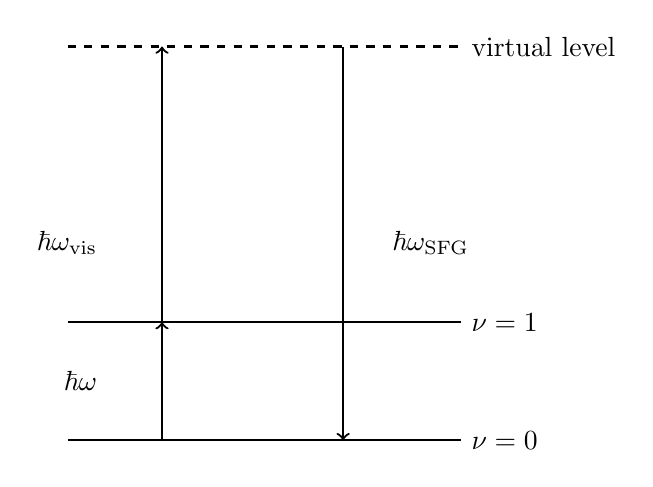
\begin{tikzpicture}[help lines/.style={thin,draw=black!50}]
%%\draw[help lines] (0,0) grid (4,4);
\draw [-, thick] (0,0) -- (5,0) node [anchor = west] {$\nu =0$};
\draw (0.5,0.75) node [anchor = east] {$\hbar\omega$};
\draw [-, thick] (0,1.5) -- (5,1.5) node [anchor = west] {$\nu = 1$};
\draw (0.5,2.5) node [anchor = east] {$\hbar\omega_{\text{vis}}$};
\draw [-, thick,dashed] (0,5) -- (5,5) node [anchor = west] {virtual level};
\draw (4.0,2.5) node [anchor = west] {$\hbar\omega_{\text{SFG}}$};
\draw [->, thick] (1.2,0) -- (1.2,1.5);
\draw [->, thick] (1.2,1.5) -- (1.2,5);
\draw [->, thick] (3.5,5) -- (3.5,0);
\end{tikzpicture}
\caption{The schematic of the VSFG process which involves IR and Raman transitions. The $\nu =0$, $\nu=1$ levels denote the ground and the first excited state of the oscillator, respectively.
 The dashed line denotes a virtual electronic state in the Raman transition.}\label{fig:sfg_1a}
\end{figure}

Because experiments usually employed visible and SFG frequencies are far from resonant 
conditions, $\chi^{(2),\text{NR}}$ can be considered totally off-resonant and therefore 
insensitive to the laser beams' frequencies involved. Therefore, we can neglect the 
frequency dependence of the non-resonant term.
The molecular information is contained in the resonant signal. The resonant susceptibility $\chi^{(2),\text{R}}(\omega)$ is given by 
\begin{equation}
  \chi_{\eta\xi\kappa}^{(2),\text{R}}(\omega)=\frac{-i}{\hbar}\int_0^\infty dt e^{i\omega t} \text{Tr}{[\rho,\mu_\kappa]\alpha_{\eta\xi}(t)},
\label{eq:chi_R}
\end{equation}
where the index $\eta$, $\xi$ and $\kappa$ are one of $x, y$ and $z$ labels of the laboratory coordinate frame.
In Eq.\thinspace(\ref{eq:chi_R}) $\rho=e^{-\beta H/Z}$ for a system with Hamiltonian $H$ and partition function $Z$ at reciprocal temperature $\beta=1/k_BT$;
$\mu_\kappa$ is the $\kappa$-th component of the system electric dipole and ${\alpha_{\eta\xi}}$ is the $\eta\xi$-th component of the polarizabiltiy tensor. [\cite{1995SM}]
Besides the vibrational resonance, $\chi^{\text{(2),R}}$, which reflects the vibrational and orientational characteristics of the surface species, 
the VSFG signal also includes the contribution from the non-resonant signal background $\chi^{\text{(2),NR}}$, 
due to static hyperpolarizability of the interface itself. [\cite{Che12}]  
For example, there are strong non-resonant second-order nonlinear responses [\cite{Pradier11,Vanselow12,Wieckowski99}] of the interface in the case of some metal(-oxide). 
Generally, experiments employ visible light and VSFG frequencies far from resonant conditions, therefore, the non-resonant 
term $\chi^{\text{(2),NR}}$ is approximately off-resonant to the light frequencies involved. [\cite{Morita02}]
%Neglecting the frequency dependence of the nonresonant term $\chi^{\text{(2),NR}}$ is usually a good approximation. 

\paragraph{Microscopic Expression of Molecular Hyperpolarizability} 
As the electric field is increased, the description of the induced dipole moment 
$\boldsymbol \mu$ should include the normally insignificant nonlinear terms. We can express the induced dipole moment as
\begin{equation}
  {\boldsymbol \mu} = {\boldsymbol \mu}_0 +\alpha {\bf E} + \beta {\bf E E}.
\label{eq:induced_mu}
\end{equation}
%or
%\begin{equation}
%  \mu_i = (\mu_0)_i +\alpha_i  E_i + \beta_{ijk}E_j E_k + \cdots.
%\label{eq:induced_mu}
%\end{equation}
The VSFG spectra are determined by the frequency-dependent hyperpolarizability in molecular level description. 
The frequency-dependent hyperpolarizability can be expressed as a sum of resonant and non-resonant terms:
\begin{equation}
\beta_{\eta\xi\kappa}(\omega_{\text{SFG}},\omega_{\text{vis}},\omega)=\beta_{\eta\xi\kappa}^{\text{R}}+\beta_{\eta\xi\kappa}^{\text{NR}},
\label{eq:beta}
\end{equation}
where $\eta$, $\xi$ and $\kappa$ are space-fixed axes.
The resonant term of the frequency-dependent hyperpolarizability is 
\begin{equation}
  \beta_{\eta\xi\kappa}^{\text{R}}(\omega_{\text{SFG}},\omega_{\text{vis}},\omega)=\sum_{v',v}\frac{\langle v|\alpha_{\eta\xi}|v'\rangle\langle v'|\mu_{\kappa}|v\rangle}{(\omega_{v'}-\omega_v)-\omega-i\gamma_{v'v}}\rho_v,
\label{eq:beta_R}
\end{equation}
where the subscripts $\eta$, $\xi$ and $\kappa$ denote body-fixed axes,
$\omega_{v'}-\omega_v$ is the vibrational energy gap, 
$\rho_v$ is the thermal distribution function of the initial vibrational states $v$,
$\alpha_{\eta\xi}$ is the $\eta\xi$-th component of the molecular dipole polarizability,
$\mu_{\kappa}$ is the $\kappa$-th component of the molecular dipole moment,
and $\gamma_{v'v}$ is the damping rate.
Since  
(see Appendix \ref{calculation_of_chi}) 
\begin{align}
\int_0^\infty dt e^{-it((\omega_{v'}-\omega_v)-\omega-i\gamma_{v'v})}=\frac{-i}{(\omega_{v'}-\omega_v)-\omega-i\gamma_{v'v}},
\label{integral_identity1a}
\end{align}
we can rewrite Eq.\thinspace(\ref{eq:beta_R}) as 
\begin{align}
  \beta_{\eta\xi\kappa}^{\text{R}}&=i\int_0^\infty dt \sum_{v'v}e^{-i[(\omega_{v'}-\omega_v)-\omega-i\gamma_{v'v}]t} \langle v|\alpha_{\eta\xi}|v'\rangle\langle v'|\mu_{\kappa}|v\rangle \rho_v \nonumber\\
   &=i\int_0^\infty dt \sum_{v'v}e^{i\omega t} \langle v|e^{iHt}\alpha_{\eta\xi}e^{-iHt}|v'\rangle\langle v'|\mu_{\kappa}|v\rangle \rho_v \nonumber\\
   &=i\int_0^\infty dt e^{i\omega t} \langle\alpha_{\eta\xi}(t)\mu_{\eta\xi}(0)\rangle,
\label{eq:beta_R_b}
\end{align}
where $H$ is the Hamiltonian of the system without external field. 
Eq.\thinspace(\ref{eq:beta_R_b}) indicates that the resonant term $\beta_{\eta\xi\kappa}^{(2),\text{R}}$ is the Fourier-Laplace transformation of the quantity $\langle\alpha_{\eta\xi}(t)\mu_{\kappa}(0)\rangle$, i.e., the ensemble average of the time correlation function $\alpha_{}(t)\mu_{r}(0)$.
The damping rate $\gamma_{v'v}$ is not explicitly included in Eq.\thinspace(\ref{eq:beta_R_b}), because the dephasing is incorporated in the time development of the off-diagonal matrix elements 
of $\alpha_{\eta\xi}(t)$ and $\mu_{\kappa}(0)$.

The $\chi^{(2),R}_{\eta\xi\kappa}$ is microscopically represented as the average sum of first-order hyperpolarizability of the constituent molecules $\beta$ in the space-fixed frame
\begin{align}
  \chi^{(2),R}_{\eta\xi\kappa} = \langle \sum_i^N \sum_{pqr} D_{\eta p}(\Omega_i) D_{\xi q}(\Omega_i) D_{\kappa r}(\Omega_i) \beta_{pqr}\rangle
\label{average_sum}
\end{align}
where $D(\Omega_i)$ is the direction cosine matrix of the $i$-th molecule, projecting $\beta$ onto the space-fixed frame. [\cite{Morita2000}]

%and evaluate it with the static hyperpolarizability, which can be calculated by an \abinitio Molecular Orbital (MO) package\cite{Morita02}, 
%\begin{equation}
%        \beta_{\eta\xi\kappa}^{\text{NR}}=\sigma\beta_{\eta\xi\kappa}^{\text{static}},
%\label{eq:beta_NR}
%\end{equation}
%where $\sigma$ is the symmetry number among the indices $\eta$, $\xi$ and $\kappa$.
%\paragraph{Derive the value of $\sigma$}
%The frequency-dependent hyperpolarizability, $\beta(\omega_1,\omega_2,\omega_3)$, satisfies the following equation 
%\begin{equation}
%\label{eq:beta_condition}
%        P_p(\omega_1)=\sum_q\alpha_{pq}(\omega_1)E_q(\omega_1)+\sum_{qr}\beta_{pqr}(\omega_1,\omega_2,\omega_3)E_q(\omega_2)E_r(\omega_3)+\cdots
%\end{equation}
%where the suffices $p$, $q$ and $r$ range over $x$, $y$ and $z$, and $P_p(\omega_1)$ is the induced dipole moment at frequncy $\omega_1$. The static polarizability and hyperpolarizability are defined as 
%\begin{equation}
%        \alpha_{pq}^{\text{static}}=(\frac{\partial P_p}{\partial E_q})_{E=0},\ \
%        \beta_{pqr}^{\text{static}}=(\frac{\partial^2 P_p}{\partial E_q \partial E_r})_{E=0}
%\label{eq:beta_condition}
%\end{equation}
%and thus the dipole moment in a static exteral electric field is expressed as 
%\begin{equation}
%        P_p^{\text{static}}=(P_p)_{E=0}+\sum_q\alpha_{pq}^{\text{static}}E_q+\frac{1}{2}\sum_{qr}\beta_{pqr}^{\text{static}}E_qE_r+\cdots,
%\label{eq:static_dipole_moment}
%\end{equation}
%where $(P_p)_{E=0}$ is the permanent dipole moment. From Eq. (\ref{eq:beta_condition}) and Eq. (\ref{eq:static_dipole_moment}), we obtain $\sigma=1/2$ in Eq. (\ref{eq:beta_NR}).

\paragraph{The Fresnel Factors}
Because of screening and dipole-dipole coupling, the local electric fields felt by molecules is different from the macroscopic fields. [\cite{Vanselow12}] 
The SFG signal depends on the magnitude of the local electric fields  of the the interacting optical beams at the interfaces. 
While the magnitude of the local electric fields is related to both the intensity of the incident beams and the linear refractive indices 
of the different layers (bulk) of the sample.  [\cite{Khatib16}] The Fresnel coefficients define the magnitude of the electric fields at the interface. 
Therefore, to find out the magnitude of the local electric fields, we need to evaluate the Fresnel factors. 
The SFG intensity $I_{\text{SFG}}$, is proportional to the intensities of the incident visible and infrared beams, $I_{\text{vis}}$, $I$, 
and to the square of the second-order nonlinear susceptibilities,
$\chi_{\eta\xi\kappa}^{(2)}(\omega_{\text{SFG}})$, of the interface:
\begin{equation}
        \chi_{\eta\xi\kappa}^{(2)}(\omega_{\text{SFG}})\propto|\sum_{\eta,\xi,\kappa}L_{\eta\eta}(\omega_{\text{SFG}})\chi_{\eta\xi\kappa}^{(2)}(\omega_{\text{SFG}})L_{\xi\xi}(\omega_{\text{vis}})L_{\kappa\kappa}(\omega)|^2\text{sec}^2(\theta_{\text{SFG}})I_{\text{vis}}I
\label{eq:chi}
\end{equation}
where $\eta$, $\xi$, $\kappa$ are the Descartes coordinates of the reference frame;
$\omega_{\text{SFG}}=\omega_{\text{vis}}+\omega$ is the frequency of SFG beam; 
$L_{\eta\eta}$, $L_{\xi\xi}$ and $L_{\kappa\kappa}$ are the Fresnel coefficients; 
$\theta_{\text{SFG}}$ is the reflected angle of SFG beam with respect to the normal 
direction in the medium.

\subsection{Sum Frequency Generation Spectra from Velocity-Velocity Correlation Functions}
%To construct SFG spectrum of O-H stretching at the water/vapor interface and to ascertain the molecular origin of SFG spectrum, 
%quantum corrected time correlation function \cite{Morita02,Morita04} and instantaneous normal mode (INM) methods are used 
%by Perry and coworkers.\cite{Perry03} 
%For  water/vapor interface, the INM SFG spectrum is in agreement with the time correlatin function SFG spectrum. 
%This implies that motional narrowing effects play little role  in the interfacial line shape. The Shen group suggests that 
%the motional narrowing effects may be significant in the SPS geometry, where the "free O-H" stretching peak is greatly diminished.\cite{WeiX02}
%========================
%\section{solutions}
%Here we discuss the calculation of nonlinear susceptibility of water molecules at liquid/vapor interfaces.
%The SFG spectrum is proportional to the square of the nonlinear susceptibility of water molecules at the water/vapor interface. \cite{QD94}  
%Details:
In this paragraph I review the derivation an expression for the calculation of the sum frequency generation spectra of water interfaces that is
based on the projection of the atomic velocities on the local normal modes, such an approach permits one to obtain the SFG signals from suitable
velocity-velocity ACFs, reducing the computational cost to that of the accumulation of a molecular dynamics trajectory, and therefore cutting 
the overhead costs associated with the explicit calculation of the dipole and polarizability tensor. Moreover, the method permits to interpret 
the peaks in the spectrum in terms of local modes.
The components of the resonant term $\chi^{\text{(2),R}}_{\eta\xi\kappa}$ of the second order susceptibility can be calculated 
according to the classical formula [\cite{Morita02,Morita2008,Nihonyanagi2011}]
\begin{align}
  \chi^{\text{(2),R}}_{\eta\xi\kappa}&=\frac{-i}{k_{\text{B}}T \omega} \int_0^\infty dt e^{i\omega t}\left\langle \dot{A}_{\eta\xi}(t) \dot{M}_{\kappa}(0)\right\rangle 
 \label{eq:chi}
\end{align}
%\begin{align}
% \chi^{(2)}_{XXZ,R}&=\frac{i}{k_BT \omega} \sum\limits_j \int_0^\infty dt e^{i\omega t} \left \langle \frac{\partial A_{XX}}{\partial r_j} \frac{\partial M_Z}{\partial r_j}  \dot{r}_j(0) \dot{r}_j(t) \right\rangle
% \label{eq:chi2}
% \end{align}
where $k_{\text{B}}$ is the Boltzmann constant, $\omega$ is the frequency of the IR beam, ${\bf M}$ (${A}$) are the dipole 
moment (dipole polarizability) of the system, and $\left\langle\dots\right\rangle$ denotes the average over all starting time points. 
%The derivation of Eq.\thinspace(\ref{eq:chi}) is given in Appendix \ref{calculation_of_chi}.
 
 The total dipole moment and dipole polarizability derivatives for the system can be expressed in terms of the water and bond contributions:
\begin{align}
 \dot{A}&=\sum_{i=1}^N \sum_{\epsilon}\dot{\alpha}^{i,\text{l},\epsilon} \\ 
 \dot{{\bf M}}&=\sum_{i=1}^N \sum_{\epsilon}\dot{\mu}^{i,\text{l},\epsilon} 
 \label{eq:A-M}
\end{align}
where ${\mu}^{i,\text{l},\epsilon}$ (${\alpha}^{i,\text{l},\epsilon}$) is the dipole moment (polarizability)
of the bond $\epsilon$ of the $i$-th water molecule, the superscript (l) denote these quantities are measured in the 
lab frame, and $N$ is the total number of the water molecules.
Therefore, the correlation function in Eq.\thinspace(\ref{eq:chi}) can be written as 
\begin{align}
  \langle\dot{A}_{\eta\xi}(t)\dot{M}_{\kappa}(0)\rangle 
    &=\sum_{i=1}^N \sum_{\epsilon}\left\langle\dot{\alpha}_{\eta\xi,i,\epsilon}^{\text{l}}(t)\dot{\mu}_{\kappa,i,\epsilon}^{\text{l}}(0)\right\rangle \nonumber \\ 
    &+\sum_{i=1}^N \sum_{\epsilon}\left\langle\dot{\alpha}_{\eta\xi,i,\epsilon}^{\text{l}}(t)\dot{\mu}_{\kappa,i,-\epsilon}^{\text{l}}(0)\right\rangle \nonumber \\
    &+\sum_{i,j=1;i\neq j}^N \sum_{\epsilon,\epsilon'}\left\langle\dot{\alpha}_{\eta\xi,i,\epsilon}^{\text{l}}(t)\dot{\mu}_{\kappa,i,\epsilon'}^{\text{l}}(0)\right\rangle.
 \label{eq:correl_AM}
 \end{align}
In Eq.\thinspace(\ref{eq:correl_AM}), the first term of the right-hand side is the bond auto-correlation, the second term accounts 
for the correlation between the two bonds in the same water molecule, and the third them for the correlation between 
bonds in two different water molecules.
 
We assume that the bond elongation are small compared to the total bond length and stretching frequencies of the bond are 
much larger than frequencies of bond reorientation, for example, the libration.
Therefore, we can approximately write ${\dot\mu}(0)$ by 
\begin{align}
    \dot\mu_{\kappa}(0)&=\sum_i^{x,y,z}{\bf{D}}_{\kappa i}(0)\dot{\mu}_i(0) \nonumber \\
                       &=\sum_i^{x,y,z}{\bf{D}}_{\kappa i}(0)\biggl(\sum_j^{x,y,z}\frac{d\mu_i}{d r_j}\frac{d{r}_j}{dt}|_{t=0}\biggr) \nonumber \\
                       &=\sum_{i}^{x,y,z}{\bf{D}}_{\kappa i}(0)\frac{d\mu_i}{dr_z}v_z(0),
    \label{eq:dot_mu}
 \end{align}
where ${\bf D}_{\kappa i}$ is the direction cosine between the laboratory-fixed $\kappa$ axis and the molecular-fixed $i$ axis,
and $v_z=\frac{d{r}_z}{dt}|_{t=0}$ is the projection of the velocity on the bond axis.

Similarly, for the dipole polarizability, we have
\begin{align}
  \dot\alpha_{\eta\xi}(t)&=\sum_{i,j}^{x,y,z} \biggl({\bf{D}}_{\eta i}(t)\frac{\partial\alpha_{ij}}{\partial r_z}{\bf{D}}_{\xi j}(t)\biggr)v_z(t). 
  \label{eq:dot_alpha}
 \end{align}
The Eq.\thinspace(\ref{eq:dot_mu}) and Eq.\thinspace(\ref{eq:dot_alpha}) simplify the calculation of the  
$\left\langle \dot{A}_{\eta\xi}(t) \dot{\bf{M}}_{\kappa}(0)\right\rangle$ in Eq.\thinspace(\ref{eq:chi}), because $v_z(t)$
and ${\bf{D}}(t)$ can be readily determined from the DFTMD
trajectory, and $\frac{d\mu_i}{dr_z}$ and $\frac{d\alpha_{ij}}{dr_z}$ can be parameterized. [\cite{Corcelli05,Khatib16}]
%
\begin{figure}
\centering
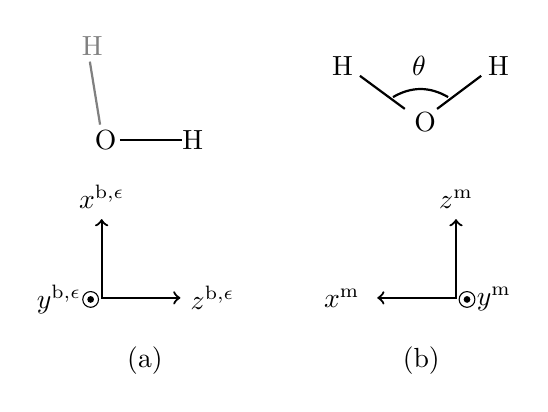
\begin{tikzpicture}[help lines/.style={thin,draw=black!50}]
%\draw[help lines] (0,0) grid (4,4);
%a
\draw [<->,thick] (0,1) node (xaxis) [above] {$x^{\text{b},\epsilon}$}
  |- (1,0) node (zaxis) [right] {$z^{\text{b},\epsilon}$};
  \filldraw[black] (-0.14,-0.02) circle (1pt) node [anchor=east] {$y^{\text{b},\epsilon}$};
\draw(-0.14,-0.02) circle (0.1);
\draw (0.2, -0.8) node [anchor=west] {(a)};
% H2O
\draw[gray,thick] (-0.02, 2.2) coordinate (a_1) -- (-0.15, 3) coordinate (a_2);
\draw[thick] (0.23, 2) coordinate (b_1) -- (1.02, 2) coordinate (b_2);
\draw (0.31, 2) node [anchor=east] {O};
\draw (0.9, 2) node [anchor=west] {H};
\draw[gray] (-0.12, 2.95) node [anchor=south] {H};
%\draw (0.56, 2.61) node {\chemfig{[:-84]H-O-[:0]H}};
%b
\draw [<->,thick] (3.5,0)--(4.5,0) node (xaxis){} 
  |- (4.5,0)--(4.5,1) node (zaxis) [above] {$z^{\text{m}}$};
  \filldraw[black] (4.64, -0.02) circle (1pt) node [anchor=west] {$y^{\text{m}}$};
\draw (2.7, 0) node [anchor=west] {$x^{\text{m}}$};
\draw(4.64,-0.02) circle (0.1);
\draw (3.7, -0.8) node [anchor=west] {(b)};
% H2O
\draw[thick] (3.85, 2.4) coordinate (a_1) -- (3.28, 2.82) coordinate (a_2);
\draw[thick] (4.26, 2.4) coordinate (b_1) -- (4.82, 2.82) coordinate (b_2);
\draw[thick] (3.7,2.55) to [out=30,in=150] (4.4,2.55);
\draw (4.03, 2.7) node [anchor=south] {$\theta$};
\draw (4.37, 2.23) node [anchor=east] {O};
\draw (5.04, 2.7) node [anchor=south] {H};
\draw (3.06, 2.7) node [anchor=south] {H};
%\draw (4.06, 2.61) node {\chemfig{[:-37]H-O-[:37]H}};
\end{tikzpicture}
  \caption{\label{fig:frameworks} The representation of the bond (a) and the molecular (b) frameworks.}
\end{figure}

%
We used three different frameworks: the lab framework ($x^{\text{l}},y^{\text{l}},z^{\text{l}}$), the molecular framework 
($x^{\text{m}},y^{\text{m}},z^{\text{m}}$) and the bond framework ($x^{\text{b}},y^{\text{b}},z^{\text{b}}$) (see Fig.\thinspace\ref{fig:frameworks} [\cite{Khatib2017}]).
In the lab framework, the $z^{\text{l}}$-axis is perpendicular to the interface. 
The molecular frame will be used to decompose the signal into normal modes of water monomers. 
For the $j$-th molecule, the $z^{\text m}$ axis is along the bisector of the H-O-H angle, the $x^{\text m}$ axis is in the molecular plane, 
and the $y^{\text m}$ axis is out of the molecular plane. [\cite{Khatib2017}] 

In the bond framework, $z^{\text{b},\epsilon}$ axis is along the bond $\epsilon$ of a molecule, $z^{\text{b},\epsilon}$
is in the molecular plane and $y^{\text{b},\epsilon}$ is out of the molecular plane.
\begin{align}
  \dot{\alpha}^{\text{l},\epsilon} &= {\bf{D}}^{\text{m}}{\bf{D}}^{\text{b},\epsilon}(\frac{\partial{\alpha}^{\text{b}}}{\partial r}\dot
    r^{\epsilon})({\bf D}^{\text{b},\epsilon})^{\text{T}}({\bf D}^{\text{m}})^{\text{T}}, \\ 
    \dot\mu^{\text{l},\epsilon} &= {\bf{D}}^{\text{m}}{\bf{D}}^{\text{b},\epsilon}(\frac{\partial \mu^{\text{b}}}{\partial r}\dot r^{\epsilon}).
    \label{eq:dot_mu-alpha}
 \end{align}
The direction cosine matrix ${\bf{D}}^{\text{b},\epsilon=1}$ and ${\bf{D}}^{\text{b},\epsilon=-1}$ can be expressed as 
\begin{equation}
    {\bf{D}}^{\text{b},1}=\left(
                \begin{matrix}
                    \text{cos}\frac{\theta}{2} &  0  & -\text{sin}\frac{\theta}{2}\\
                    0 & 1 & 0\\
                    \text{sin}\frac{\theta}{2} & 0 & \text{cos}\frac{\theta}{2}
\end{matrix}
\right),\quad
    {\bf{D}}^{\text{b},-1}=\left(
         \begin{matrix}
             -\text{cos}\frac{\theta}{2} & 0 & \text{sin}\frac{\theta}{2}\\
             0 & 1 & 0\\
             \text{sin}\frac{\theta}{2} & 0  & \text{cos}\frac{\theta}{2}
\end{matrix}
\right),
\label{eq:D_b}
\end{equation}
where $\theta$ is the H-O-H angle in a water molecule.
%The approximate value of the angle is 105.5$^\circ$.
We can use ${\bf{D}}^{\text{m}}$ to transform the coordinates in a molecular framework to coordinates in the lab framework. 
Because the orientation of water molecules is changing during the simulation, 
%the angle $\theta'_i$ between the water dipole moment and the $z$-axis is time dependent, therefore, 
${\bf{D}}^{\text{m}}$ is time dependent. 
%It can be expressed as 
%\begin{equation}
%    {\bf{D}}^{\text{m}}=
%    \left(
%        \begin{matrix}
%            \text{cos}{\gamma} & \text{sin}{\gamma} & 0\\
%            -\text{sin}{\gamma} & \text{cos}{\gamma} & 0\\
%            0 & 0 & 1
%        \end{matrix}
%     \right)
%     \left(
%         \begin{matrix}
%             \text{cos}{\theta'} & 0 & -\text{sin}{\theta'}\\
%             0 & 1 & 0\\
%             \text{sin}{\theta'} & 0  & \text{cos}{\theta'}
%         \end{matrix}
%     \right) 
%     =
%     \left(
%         \begin{matrix}
%             \text{cos}{\gamma}\text{cos}{\theta'} & \text{sin}{\gamma} & -\text{cos}{\gamma}\text{sin}{\theta'}\\
%             -\text{sin}{\gamma}\text{cos}{\theta'} & \text{cos}{\gamma} & \text{sin}{\gamma}\text{sin}{\theta'}\\
%             \text{sin}{\theta'} & 0  & \text{cos}{\theta'}
%         \end{matrix}
%     \right),
%\label{eq:D_m}
%\end{equation}
%where $\gamma$ is the angle between the incident plane (x-z plane) and the molecular plane of a water molecule,
%and $\theta'$ is the angle of the dipole moment of the water molecule from the normal direction of the interface, 
%and both $\gamma$ and $\theta'$ are time dependent.

The parametrization of $\frac{\partial \mu_{k}}{\partial r_z}$ and $\frac{\partial\alpha_{ij}}{\partial r_z}$ is based 
on the calculation of Maximally Localized Wannier Functions (MLWF) [\cite{Marzari97}] 
 and can be done through the approach developed by Salanne \etal [\cite{Salanne08}] and Khatib \etal [\cite{Khatib2017}]
The main advantage of such approximation for the calculation of the susceptibility is that still retain details of the
water/vapor interfaces including the full electronic structure, but its computational
cost is reduced with respect to a full calculation with the instantaneous evaluation of the 
molecular dipoles and polarizabilities. [\cite{sulpizi2013}] 
The implementation of this parametrization is given in Appendix \ref{calculate_derivatives}.
%\paragraph{Calculation of $\chi^{(2)}$ (Method 2)}
%We now consider the velocities projection on the water normal modes, identified by the collective variables ${\bf{R}}_j$ in the molecular framework. 
%The single water molecule has nine normal modes. Six of them have the angular frequencies $\omega$ equal zero and three normal modes remains. 
%The three normal modes are the symmetric stretching (SS), the antisymmetric stretching (AS) and the bending (B).
%The dipole moment and the molecular polarizability of the $i$th water molecule can be rewritten as
%\begin{align}
%    \dot{\bf \alpha}_{i}^{\text{l}}(t)&={\bf{D}}_{\text{m},i}(\sum_{j=Q,SS,AS}\frac{\partial{\bf\alpha}_{i}^{\text{m}}}{\partial R_j}){\bf{D}}^{\text{T}}_{\text{m},i}, \\ 
%    \dot{\bf \mu}_{i}^{\text{l}}&={\bf{D}}_{\text{m},i}(\sum_{j=Q,SS,AS}\frac{\partial{\bf\mu}_i^{\text{m}}}{\partial R_j}\dot{R}_j).  
%    \label{eq:dot_mu_alpha}
%\end{align}
%where $i$ denote the $i$-th water molecule.
%To parametrize the derivatives $\frac{\partial \alpha_i^{\text{m}}}{\partial R_j}$ and $\frac{\partial {\bf{\mu}}_i^{\text{m}}}{\partial R_j}$,
%the Maximally Localized Wannier Functions (MLWF) were emplyed.\cite{Salanne08,Khatib2017}
 
\chapter{Experimental SFG spectra of salty interfaces}\label{CHAPTER_SFG_Exp}
In this chapter, we give the experimental results obtained on salty solutions containing alkali cations and nitrate (iodide) anions. \cite{PS03,AJ12,HuaWei2014} 

%We will choose the interface of lithium nitrate solution as our research object, which is a typical example of the interface of alkali metal nitrate solution.
From the experimental data of surface tension dependence on solute concentration $\text{d}\gamma/\text{d}m_2$ 
at low electrolyte concentrations ($\leq$1.5 M ), \cite{Weissenborn95,Hey81,Jarvis68,Jarvis72} 
%and the assumption that \Na is the most excluded cation
the relation of the surface/bulk molar concentration ratio $K_{\text{p}}$ \cite{Pegram2006} among \li, \Na and \K is: 
\begin{equation}
0=K_{\text{p,Na}^+}< K_{\text{p,K}^+}< K_{\text{p,Li}^+}.
\label{eq:bscr}
\end{equation}
i.e., \Na is the most surface-excluded in the water solution RNO$_3$, \K is less excluded, 
and \Li is the least excluded cation. (See Appendix \ref{surface_tension_increment} for details.)
In modeling the interfaces of aqueous solutions of alkali metal nitrates, we decided to start with LiNO$_3$, because the \Li ion is the least excluded of the vapor-liquid interface 
among the alkali metal ions. 
%
%The aim of our work here is to provide a molecular picture 
%for the water/vapor interface of the \ch{LiNO3}-containing solution 
%to interpret the experimental spectra. In particular a question raises if simple models 
%for the solvated ion clusters can already provide information
%on the ions-water complexes formed at the interface. 
%It is known that nitrate (\nitrate) is a naturally occurring ion which is part of the nitrogen cycle, 
%and it can reach both surface water and groundwater as a consequence of agricultural activity. 
%Nitrate also has effects on human health,  because of the toxicity caused by its reduction to nitrite (NO$_2^-$). \cite{WHO11}
%The biological effect of nitrite in humans is its involvement in the oxidation of
%normal Hb to metHb, which is unable to transport oxygen to the tissues.
%For example, infants who drink water with high levels of nitrate (more than 10 mg/L) may suffer 
%a serious health condition due to blue baby syndrome.\cite{Knobeloch00}
%

%The goal of this chapter is to find the origin of the main characteristics of the VSFG spectra of the \LiN solution,
%and provide a molecular picture to interpret the recorded spectra.
%In order to achieve this goal, we simulate water/vapor interface including \Li and \nitrate, 
%as shown in Fig.\thinspace\ref{fig:interface_chandler},
%and extract the vibrational spectroscopic properties of the water/vapor interface of LiNO$_3$ solution.
%=========
%
%\begin{figure}[htbp]
%\centering
%\includegraphics [width=0.5 \textwidth] {./diagrams/interface_chandler}
%\setlength{\abovecaptionskip}{0pt}
%\caption{\label{fig:interface_chandler} The water/vapor interfaces of \LiN solution and pure water. 
%The right panel shows that the \Li and the \nitrate ions are separated by a water molecule at the salty interface.}
%\end{figure}
%The water molecules below 4 \AA  of the instantaneous interfaces are shown opaquely. 

%
Hua \etal \cite{HuaWei2014} have recently measured the VSFG spectra of water/vapor interface of \LiN salt solutions in the OH stretching region
(3000--3800 \centimeter) using Heterodyne Detected VSFG spectroscopy. \cite{HuaWei2011,HuaWei2011b,ChenXiangKe2010} 
The experimental result of the VSFG intensity of the alkali nitrate interfaces is given by in Fig.\space\ref{fig:Allen12}. 
At a difference with the spectra for the water interface, in the spectra of 
\LiN solutions, a depletion of the 3200 \cm peak is observed, with an 
enhancement of the 3400 \cm peak.
A similar behaviour had been observed for the interface of NaNO$_3$ and 
Mg(NO$_3$)$_2$ solutions. \cite{AJ12,HuaWei2014} It has been 
suggested that this depletion of the 3200 \cm peak, and in some cases 
the enhancement of the 3400 \cm peak, is an indication that nitrate 
ions reside at the interface. On the other hand the small 
cations should have little surface propensity. 
It has also been argued that the positive electric field found at the interface of NaCl, NaI and 
NaNO$_3$ salt solutions is due to the formation of an ionic double layer 
between anions located near the surface and their counter-cations (e.g.
Na$^+$) located further below. In Phase-Sensitive (PS) VSFG experiments the 
magnitude of the induced change in the Im$\chi^{(2)}$ spectra comparatively
to that of the neat water suggested that \nitrate has a surface propensity 
just in between I$^-$ and Cl$^-$. \cite{Verreault2013,Verreault2009} 
% exp. results.
\begin{figure}[H] %[htbp]
\centering
  \includegraphics [width=0.6 \textwidth] {./diagrams/vsfg_alkali_nitrate}
\setlength{\abovecaptionskip}{0pt}
  \caption{\label{fig:Allen12}Experimental VSFG intensity of \LiN solutions, compared with that of neat water. \cite{HuaWei2014}}
\end{figure}

%\begin{figure}[htbp]
%    \centering
%    \begin{tikzpicture}
%        \begin{axis}[
%        scale=0.8, % scale the figure but the labels
%        /pgf/number format/.cd,
%        %use comma,
%        1000 sep={}, % separator of thousands
%        legend style={draw=none},
%        legend pos=north west,
%        %title=VSFG Intensity,
%        xlabel={Wave Number (cm$^{-1}$)},
%        every axis x label/.style={
%        at={(rel axis cs: 0.5, -0.20)},
%        anchor=center}, 
%        ylabel={Intensity (Arb. Unit)},
%        every axis y label/.style={    
%        at={(rel axis cs:-0.18, 0.5)},rotate=90,
%        anchor=center}, 
%        ymin=0,
%        ymax=0.3,
%        minor y tick num=1,
%        ]
%        \addplot[mark=x, black,domain=3000:3800,very thick]table{./chapters/chap4/data/Net_water.dat};
%        \addlegendentry{Neat Water}
%        \addplot[mark=*, blue,domain=3000:3800,very thick]table{./chapters/chap4/data/LiNO3.dat};
%        \addlegendentry{1M  \LiN}
%      \end{axis}
%   \end{tikzpicture}
% \setlength{\abovecaptionskip}{0pt}
%  \caption{\label{fig:Allen12}Experimental VSFG intensity of \LiN solutions, compared with that of neat water.\cite{HuaWei2014}}
% \end{figure}
 
  \chapter{Alkali Nitrate Clusters}\label{CHAPTER_results_clusters}
  In this chapter, gas phase clusters including alkali cations, nitrate ions and a few water molecules have been used to understand the
  effects of alkali cations and nitrate anions on hydrogen
  bonding. [\cite{jiangling2010,heine2015}] 
  VDOS is used to extract the vibrational signatures for the water molecules in these systems.
  In the first two paragraphs the effect of the anion and the cation are separately investigated. 
  The two clusters, NO$_3^-$(H$_2$O)$_3$ and \li(H$_2$O)$_4$, are used 
  to study the structural and dynamical properties of water clusters with nitrate ions and with alkali cations at $T= 300$ K. 
  In paragraph \ref{paragraph_clusters_alkali_nitrate_and_water_molecules}, the effects of the alkali metal cations 
  and the nitrate anion are discussed within clusters containing both cations and anions and an increasing number of water molecules.
  %
  \section{Cluster of Nitrate and Water Molecules}\label{paragraph_3w_nitrate}
  %EXAMPLE of FORMULA
  %$$X_n=X_k \qquad\hbox{if and only if}\qquad Y_n=Y_k \quad\hbox{and}\quad Z_n=Z_k.$$
  
  %\begin{wrapfigure}{l}[0.05cm]{8.0cm}
  %\centering
  %\includegraphics[width=0.3\textwidth]{./diagrams/3_NO3_small}
  %\setlength{\abovecaptionskip}{10pt}
  %\caption{The geometry optimized structure of the cluster NO$_3^-$(H$_2$O)$_3$. The red dotted lines denote the H-bonds.}\label{fig:3_NO3_small}
  %\end{wrapfigure}
  \begin{figure}
  \centering
  \includegraphics[width=0.5\textwidth]{./diagrams/clusters_4}
  \setlength{\abovecaptionskip}{0pt}
    \caption{\label{fig:clusters_4}The geometry optimized structure of the clusters: (a) NO$_3^-$(H$_2$O)$_3$; (b)RNO$_3$(H$_2$O)$_3$; (c) RNO$_3$(H$_2$O)$_4$; (d) RNO$_3$(H$_2$O)$_5$ (R=Li,Na,K). More structural properties are shown in Appendix \ref{structure_of_clusters}.}
  \end{figure}
  First, we consider the water cluster with a nitrate ion, NO$_3^-$(H$_2$O)$_3$. The symmetric isomer of the cluster, 
  as shown in Fig.\thinspace\ref{fig:clusters_4}(a), is obtained by geometry optimization at the BLYP/TZV2P level of theory. 
  According to the definition of the H-bond, [\cite{JT90,SB02}] there are three H-bonds in it,
  i.e., only one of the two OH bonds is H-bonded to \nitrate in each water molecule. 
  Therefore, for each water molecule, we say there is one HB and one quasi-HB.
  %The three water molecules in the cluster NO$_3^-$(H$_2$O)$_3$ have similar dynamical properties.
  Therefore, the two OH bonds in each water molecule exhibit different vibrational features. 
  Fig.\thinspace\ref{fig:vdos_NO3-3w_2_H6H7} shows the difference of VDOS for the OH bonds in the cluster.
  %(MS:repetition)It shows that both H atoms have two vibrations modes, but the two H atoms in a water molecule in the cluster prefer to vibrateing differently.
  For each water molecule, one OH bond is vibrating in the frequency range 3680--3700 cm$^{-1}$, 
  while the other in the frequency range 3380--3440 cm$^{-1}$. 
  The difference of frequencies between the vibrational modes is about $\Delta\nu=$ 250 \centimeter.
  %
  \begin{figure}[b!] %[htbp]
  \centering
  \includegraphics [width=0.6\textwidth] {./diagrams/vdos_NO3-3w_2_H6H7_simple}%
  \setlength{\abovecaptionskip}{0pt}
    \caption{\label{fig:vdos_NO3-3w_2_H6H7} The VDOS for the two OH bonds in w1 (Fig.\thinspace\ref{fig:clusters_4}(a)) of NO$_3^-$(H$_2$O)$_3$.} 
    %The length of the DFTMD trajectory is 5 ps.
  \end{figure}  %(Calculated from the function vdos3.f and ft$\_$5s.sh)
  %(MS:repetition)A quasi-HB is formed if the O--H distance $r_\text{OH}$ satisfies the condition $r_\text{OH}<3.5$ \AA, but not that the O--H$\cdots$O angle is less than $\frac{\pi}{6}$. \cite{JT90} 
  Additionally, we label the three water molecules as w1, w2, and w3, respectively (Fig.\thinspace\ref{fig:clusters_4}(a)). 
  For the three water molecules, we can find some difference in the structural parameters.
  Table\thinspace\ref{tab:3_nitrate_bond} gives the calculated lengths of H-bonds in the cluster NO$_3^-$(H$_2$O)$_3$. 
  The average differences $\Delta{d}$ between the H-bonds and the quasi-H-bonds are 0.69 \AA (Table\thinspace\ref{tab:3w_nitrate}). 
  %\paragraph{Lengths of Hydrogen Bonds}
  %[(I deleted this paragraph, because now i am not sure on this idea.) To find the possible source of the different 
  %vibrational features of water molecules in the clusterNO$_3^-$(H$_2$O)$_3$, we considered the structural properties and VDOS for water molecules in this cluster. 
  %=============
  %\begin{table}
  %\centering
  %\caption{\label{tab:3_nitrate_bond}%
  %The lengths of H-bonds in the cluster NO$_3^-$(H$_2$O)$_3$. The indices of H atoms: H6, H7 in w1; H9, H10 in w2 and H12, H13 in w3.} 
  %\begin{tabular}{ccc} \\\toprule
  % HBs& $r_a\pm\delta$ (100 K)(\A) & \multicolumn{1}{c}{ $r_a\pm\delta$ (300 K)}(\A)\\
  %\hline
  % H6-O2 &2.75$\pm$0.62& 2.40$\pm$0.52 \\
  % H7-O4 &2.79$\pm$0.58& 3.02$\pm$0.72 \\
  % H9-O3 &2.89$\pm$0.60 &2.56$\pm$0.48 \\
  % H10-O4 &2.74$\pm$0.49&3.20$\pm$0.41 \\
  % H12-O3 &2.46$\pm$0.45&2.29$\pm$0.47 \\
  % H13-O2 &2.75$\pm$0.59 &3.11$\pm$0.72
  %\end{tabular}
  %\end{table}
  %===================
  %\begin{figure}[htbp]
  %\centering
  %\includegraphics [width=0.5\textwidth] {./diagrams/gdr_ON-wat--3_NO3_Sans} 
  %\setlength{\abovecaptionskip}{20pt}
  %\caption{\label{gdr_ON-wat--3_NO3_Sans}The nitrate O ($\text{O}_\text{n}$)--water O ($\text{O}_\text{w}$) and nitrate O--water H ($\text{H}_\text{w}$) RDFs for the cluster NO$_3^-$(H$_2$O)$_3$.
  %The peaks for the former are 1.93, 2.95 and 3.95 \A, and for the later are 2.95 and 4.80 \A.}
  %\end{figure} 
  %==================================================================================
  %When $T=300$ K, the difference $r_a$ between different hydrogen atoms in one water molecule is
  %$\Delta{r_a}=0.69$ \AA, while $\Delta{r_a}=0.13$ \AA for $T=100$ K.
  %It shows that the vibrational peaks for the three water molecules are much closer than that at the higher temperature 300 K. 
  %
  %The calculated VDOS for water molecules in the cluster 
  %at a lower temperature 100 K is given in Fig.\thinspace\ref{fig:vdos_LiNO3-3w_100K_w1-2-3_font35}. 
  %At the lower temperature,
  %the 3 water molecules are more symmetric distributed bound to the central nitrate.
  %Therefore, the difference between H-bonds in the symmetric isomer of NO$_3^-$(H$_2$O)$_3$ is likely a finite temperature effect, which can be verified by the calculation of the VDOS for water molecules.
  %
  %Both differences $\Delta\nu$ and $\Delta{d}$ decrease as the temperature decrease,
  %Therefore, the different vibrational features are temperature-dependent effect. 
  %--------------------
  %\begin{figure}[htbp]
  %\centering
  %\includegraphics [width=0.5 \textwidth] {./diagrams/vdos_LiNO3-3w_100K_w1-2-3_font35} 
  %\setlength{\abovecaptionskip}{20pt}
  %\caption{\label{fig:vdos_LiNO3-3w_100K_w1-2-3_font35} The VDOS $g(\nu)$ for water 
  %molecules in the cluster NO$_3^-$(H$_2$O)$_3$ at 100 K shows that 
  %the vibrational peaks for the three water molecules are very close to each other ($\Delta\nu <$ 10 \cm)for both vibrational and bending modes.}
  %\end{figure}
  %====================================================================================
  %In addition, the VDOS for H atoms and water molecules in NO$_3^-$(H$_2$O)$_3$ (Fig.\thinspace\ref{fig:vdos_NO3-3w_2_H-wat}) shows that H's contribution dominates that of the water molecule. 
  %\begin{figure}[htbp]
  %\centering
  %\includegraphics [width=0.5\textwidth] {./diagrams/vdos_NO3-3w_2_H-wat}%
  %\setlength{\abovecaptionskip}{20pt}
  %\caption{\label{fig:vdos_NO3-3w_2_H-wat}The comparison between the VDOS for H and of a whole water molecule, for a water molecule ({w1}, Fig. ~\ref{fig:3_NO3_small}), 
  %in NO$_3^-$(H$_2$O)$_3$ at 300 K.}
  %\end{figure}  %(Calculated from the function vdos3.f and ft$\_$5s.sh)
  %============
  %section 4_Li
  %============
  \section{Cluster of Alkali Metal Cation and Water Molecules}
  \begin{wrapfigure}{l}[0.05cm]{6.5cm}
  \centering
  \includegraphics[width=0.25\textwidth]{./diagrams/4_Li}
  \setlength{\abovecaptionskip}{0pt}
  \caption{\label{fig:4_Li}The cluster Li$^+$(H$_2$O)$_4$.}
  \end{wrapfigure}
  %====
  To find the effects of alkali cations on the structural properties of water, we investigate the cluster \li(\wat)$_4$ 
  (Fig.\thinspace\ref{fig:4_Li}). We concentrate on two aspects: the radial distribution function (RDF), 
  and the VDOS for water molecules of this cluster.

  The sharp peaks in the RDF given in Fig.\thinspace\ref{gdr_4_Li} show that the solvation shell of \Li is bound to all the four water molecules.
  The peak for $g_{\text{LiO}}$ is at 2.02 \AA, and for $g_{\text{LiH}}$ is 2.69 \AA. 
  \begin{figure}[b!]
  \centering
  \includegraphics[width=0.6\textwidth] {./diagrams/gdr_4_Li}
  \setlength{\abovecaptionskip}{0pt}
    \caption{\label{gdr_4_Li} The RDFs $g_{\text{Li-O}}$ and $g_{\text{Li-H}}$ for the cluster \li(H$_2$O)$_4$.} 
  \end{figure}
  %
  \begin{figure}[htbp]
  \centering
  \includegraphics [width=0.6\textwidth] {./diagrams/vdos_4_Li} 
  \setlength{\abovecaptionskip}{0pt}
  \caption{\label{vdos_4_Li} %old version: vdos_4_Li-wat_2p 
    The VDOS for the four water molecules (all water molecules) in the cluster \li(\wat)$_4$.} 
  %(a) The VDOS for all water molecules (black line), Li-bound (red) and H-bonded water molecules (blue).
  %(b) The VDOS for H-bonded water molecules (blue), and of both Li-bound and H-bonded water molecules (orange). }
  \end{figure}
  %

  The VDOS for water molecules in the cluster \li(\wat)$_4$ is calculated from a 20-ps trajectory,
  during which one water molecule escaped from the bonding of the \Li and then formed a new HB to 
  another water molecule. First, Fig.\thinspace\ref{vdos_4_Li} 
  shows that, in this case, there are two types of OH stretching modes in \li(\wat)$_4$ cluster:
  free OH stretch which peaks at 3705 \cm and bonded OH stretch at 3625 \centimeter. 
  However, the water molecules just bound to \Li has two degenerate free O-H stretching modes. 
  %Second, Fig.\thinspace\ref{vdos_4_Li}  shows that if a H-bonded water molecule is in the solvation shell of \Li, 
  %the H-bonded OH streching frequency is 75 \cm higher than that of the H-bonded OH strech outside the solvation shell of \Li. 
  %
  \begin{figure}[htbp]
  \centering
  \includegraphics [width=0.6 \textwidth] {./diagrams/vdos_4_Li-wat_w1_5ps} 
  \setlength{\abovecaptionskip}{20pt}
  \caption{\label{vdos_4_Li-wat_w1_5ps} 
    The VDOS for the water molecules bound to Li$^+$ (three water molecules) 
    in the cluster \li(\wat)$_4$.} 
  \end{figure}
  %
The VDOS for water molecules only bound to \Li (Fig.\thinspace\ref{vdos_4_Li-wat_w1_5ps}) shows that these water molecules only have free OH stretch, 
  since there is only a broad stretching mode at 3705 cm$^{-1}$.

  \section{Clusters of Alkali Nitrate and Water Molecules}\label{paragraph_clusters_alkali_nitrate_and_water_molecules}
  %\begin{wrapfigure}{r}[0.05cm]{7.5cm}
  %\centering
  %\includegraphics[width=0.3\textwidth]{./diagrams/3_RNO3}
  %\setlength{\abovecaptionskip}{10pt}
  %\caption{\label{fig:3_RNO3}The clusters RNO$_3$(H$_2$O)$_3$ (R=Li, Na, K).}
  %\end{wrapfigure}
  %===================
  %MS:INSERT AN INTRO:
  %===================
  As a first minimal model system for the interfaces of alkali nitrate solution, we consider alkali nitrate water clusters including 3,4,5 waters. 
  The idea is to investigate the effect of the alkali nitrate on the vibrational properties of those water molecules which are directly 
  H bonded to the ions.
  In our simulations, the clusters are geometry optimized and the most stable configurations are determined (Fig.\thinspace\ref{fig:clusters_4}(b)(c)(d)).
  The first interesting result is that for all the clusters containing 3 to 5 water molecules, a contact ion pair is maintained during the 
  300 K simulation trajectories where a direct interaction involves the cation and one of the nitrate oxygen's. 
  %The most stable isomer of the RNO$_3$(NO$_3$)$_3$ complex (R=Li,Na,K) is shown in Fig.~\ref{fig:clusters_4}(b) and compared to the symmetric slovation of the simple NO$_3$(H$_2$O)$_3$. 
  %Independently of the type of alkali cations (Li,Na,K), the most stable structure is the same.

In the LiNO$_3$(H$_2$O)$_3$ cluster, there are three H-bonds and three Li-O bonds. 
The average lengths of them are given in Table\thinspace\ref{tab:table_lino3}. 
We use HB1, HB2 and HB3 to denote the HB between w1 and w2, w2 and \nitrate, and w3 and \nitrate, 
respectively (Fig.\thinspace\ref{fig:clusters_4}(b)). Both the average lengths of HB1 and HB3 are very close 
to each other and both of them are smaller than those of HB2. 
Since both w1 and w2 are bound to \li, we calculate an average value $\bar{d}_{\text{HB}}=1.81$ \AA of the lengths of HB1 and HB3.
The difference between length of HB2 and $\bar{d}_{\text{HB}}$ is $\delta d_{\text{HB}}=0.19$ \AA.
By testing the difference of environment of each H-bonds,  we obtain that $\delta d_{\text{HB}}$ comes from the 
difference between Li-O  and H-bonds.
\begin{table}[htbp]
\centering
\caption{\label{tab:table_lino3}%
  The average length $r_a$ of H-bonds (Li-O bonds) in the cluster LiNO$_3$(H$_2$O)$_3$.}
\begin{tabular}{ccc}
Bonds& $r_a$( \AA) \\ 
\hline
HB1 &1.83 $\pm$ 0.14\\
HB2 &2.00 $\pm$ 0.25 \\
HB3 &1.79 $\pm$ 0.16 \\
O(w1)-\Li &1.95 $\pm$ 0.09 \\
O(w3)-\Li &1.92 $\pm$ 0.07 \\
O(\nitrate)-\Li &1.91 $\pm$ 0.08
\end{tabular}
\end{table}
%\subsection{Structural Characterization}
The RDF between the alkali (\li, \na\space or \pot) and the water O (panel (a)) and the nitrate O -- water H (panel (b)) are also reported in Fig.\thinspace\ref{fig:gdr_3_RNO3}. 
The sharp peaks in the RDF (Fig.\thinspace\ref{fig:gdr_3_RNO3} (b)) 
show that \nitrate is solvated and in particular a stronger HB is formed in the presence of the cation. 
%=============
%MS: added XXX
% To express number ranges like 2--4, use en-dash, which can be implemented by typing two hyphens (--).
%=============
 The vibrational features associated to the small clusters are calculated from the VDOS and reported in
Fig.\thinspace\ref{fig:vdos_Li_Na_K-NO3-3w}.
In the frequency range 3000--3800 \centimeter, each water molecules has two vibrational bands. In addition
to the free OH peak at 3700 \centimeter, we can see that the HB band is characterized by quite strong red-shifted 
peaks around 3200 \centimeter. These red-shifted peaks are associated to water molecules which are bound either to 
the cation or to both cation and anion and are different with respect to the peaks associated to the water molecules
which only bound to NO$_3^-$ in the simple NO$_3^-$(H$_2$O)$_3$ cluster (3430 \centimeter, see e.g., in Fig.\thinspace\ref{fig:vdos_NO3-3w_2_H6H7}). 
%
\begin{figure}[h!]
\centering
  \includegraphics [width=\textwidth] {./diagrams/gdr_3_RNO3}
\setlength{\abovecaptionskip}{0pt}
\caption{\label{fig:gdr_3_RNO3} (a) The RDF $g_{\text{R-O}}$ for clusters RNO$_3$(H$_2$O)$_3$ (R=Li, Na, K);
  (b) The RDF $g_{\text{O-H}}$ for clusters RNO$_3$(H$_2$O)$_3$ and NO$_3^-$(H$_2$O)$_3$ (no alkali metal cation).}
\end{figure}
%
\begin{figure}[htbp]
\centering
\includegraphics [width=1.2\textwidth, center] {./diagrams/vdos_LiNO3-3-5w}
\setlength{\abovecaptionskip}{0pt}
\caption{\label{fig:vdos_LiNO3-3-5w}The VDOS for each water molecule in the cluster LiNO$_3$(H$_2$O)$_n$: 
  (a) $n=3$;  (b) $n=4$; (c) $n=5$.
  w1: H$_2$O bound to Li$^+$ and \water;
  w2: H$_2$O bound to NO$_3^-$ and \water;
  w3: H$_2$O bound to Li$^+$ and \nit;
  w4: H$_2$O bound to \water;
  w5: H$_2$O only bound to Li$^+$.}
%w1 : the water molecule bonded to \Li and \water,
%w2 the water molecule bound to \nitrate and \wat, 
%and w3 the water molecule bound to \Li and \nit.
\end{figure}
%
\begin{figure}[htbp]
 \centering
 \includegraphics [width=1.2\textwidth, center] {./diagrams/vdos_Li_Na_K-NO3-3w}
 \setlength{\abovecaptionskip}{0pt}
  \caption{\label{fig:vdos_Li_Na_K-NO3-3w}The VDOS for water molecules in clusters (a) LiNO$_3$(H$_2$O)$_3$, (b) NaNO$_3$(H$_2$O)$_3$ and (c) KNO$_3$(H$_2$O)$_3$.  
 w1: \water bound to R$^+$ and water;
 w2: H$_2$O bound to \nitrate and \water;
 w3: \water bound to R$^+$ and \nit.
 } 
\end{figure}
%

To explore the effect of adding some additional water molecules to
the cluster, we considered the clusters RNO$_3$(H$_2$O)$_n$ ($n$=4, 5; R=Li, Na, K).
The most stable configurations are shown in Fig.\thinspace\ref{fig:clusters_4}(c) and (d),
and the corresponding VDOS for the water molecules are shown in
Fig.\thinspace\ref{fig:vdos_LiNO3-3-5w}(b) and (c) for the clusters LiNO$_3$(H$_2$O)$_n$
($n$=4 and 5). We find that the OH stretching peaks in the HB region are also quite red-shifted.
The red shift is particularly strong for the water molecules which are directly interacting with
the Li$^+$ and those which are simultaneously bound to the Li$^+$ and to the NO$_3^-$ oxygen's (e.g. w3).

%
%In the frequency range 2800--3800 \centimeter, each water molecule has two vibrational bands. In addition to the free OH peak at 3700 \centimeter, we can see that the HB band is 
%characterized by quite strong red-shifted peaks around 3200 \centimeter.
%These peaks are associated to water molecules which are bound either to the cation or to both cation and anion and 
%are different with respect to the peaks associated to the water molecules which only bound to \nitrate in the simple 
%NO$_3^-$(H$_2$O)$_3$ cluster (3460 \centimeter, Fig. ~\ref{fig:vdos_Li_Na_K-NO3-3w_roman_font40}(b) ).
%Compared with the VDOS for NO$_3^-$(H$_2$O)$_3$, the bending modes of the water molecules in RNO$_3$(H$_2$O)$_3$ are redshifted slightly. The OH stretching modes of water molecules bounded to the alkali cation in RNO$_3$(H$_2$O)$_3$ are redshifted ($|\Delta\nu|>200$ \centimeter)(b).

We also calculate the effects of other alkali metal cations, namely Na$^+$ and K$^+$. 
The calculated VDOS for water molecules in clusters NaNO$_3$(H$_2$O)$_3$ and KNO$_3$(H$_2$O)$_3$ are shown in 
Fig.\thinspace\ref{fig:vdos_Li_Na_K-NO3-3w} (b) and (c), respectively. As in the case of LiNO$_3$(H$_2$O)$_3$, the HB 
bands are also characterized by red-shifted peaks around 3200 \centimeter.
In addition, the peaks in the OH-stretching region are also compatible with infrared predissociation
(IRPD) spectra which have been recorded for the Li$^+$(H$_2$O)$_{3-4}$Ar
clusters [\cite{rodriguez2011, Miller2008, miller2010b}]
and for Na$^+$(K$^+$)(H$_2$O)$_{4-7}$ clusters, [\cite{beck2011}] although there no
nitrate is present and only the effect of the cation was investigated.

To summarize, the vibrational spectra from the clusters clearly point to red-shifted peaks which are not 
recorded in the vibrational sum-frequency generation spectra at the water/vapor interface for the \LiN solutions. 
Therefore, these small clusters cannot be directly used to describe the topmost layer of the \LiN solution, 
and we need to build more realistic models to capture the main features the interface. 
In particular, according to the cluster picture one would be tempted to rule out the possibility of a contact 
ion pair at the interface.

 
\chapter{Hydrogen bond dynamics at the water/vapor interface}\label{CHAPTER_HBD}
Hydrogen bonds play a critical role in the behaviour of bulk water\cite{Eisenberg1969,Luzar1996,Cabane2005}, 
aqueous solutions\cite{Naslund2005}, and water near interfaces\cite{Chowdhary2008}.
There are many methods to study the HB dynamics in water, solutions and interfaces, 
such as molecular dynamics simulation\cite{Tongraar2006,Chanda2006,Tongraar2010,Chowdhary2008,Banerjee2016}, neutron scattering\cite{ChenSH1984,Teixeira1990}, 
IR spectroscopy\cite{Werhahn2011,Fournier2016}, 2D-IR spectroscopy\cite{Auer07,Kim2009} and 2D-SFG spectroscopy\cite{ZhangZhen2011}.
In this chapter, we will use the general concepts and methods of HB dynamics \cite{AL96,Luzar1996,DC87} introduced in Paragraph \ref{para:def_HBP} 
in Chapter \ref{CHAPTER_Methods} to analyze the structure and dynamic properties of bulk water and the water/vapor interface. 

%
\FloatBarrier
\section{Dynamical properties of H-bonds in bulk water and at the water/vapor interface}
The bulk water and the interface between pure water and vacuum, i.e., the water/vapor interface, 
are considered in this paragraph.
%For bulk water, we can compare the results of the method in this paragraph with that of previous works\cite{AL96,Kessler2015}. 
%After the validation for bulk water, we will show in this paragraph the results of the HB dynamics of the water/vapor interface.
%[all the data on the simulation]
All simulations in this chapter were performed at 300 K within the canonical (NVT) ensemble.
The BLYP exchange and correlation functional\cite{Becke1988,LeeC1988}, 
and the D3 dispersion corrections\cite{Grimme2010,Klimes2012} have been employed.
The electron-ion interactions are described by GTH pseudopotentials\cite{Hartwigsen1998,Lippert1999}.
The length of the trajectory is 60 ps of physical time.
%The definition of $h(t)$ is based on specific H--O bond, instead of water-water pairs.
The simulated bulk water consisted of 128 water molecules in a periodic cubic box of length L = 15.64 \A, which corresponds to a density of 1.00 g cm$^{-3}$.
The simulated water/vapor interface consisted of 128 water molecules in a periodic box with size 15.64 $\times$ 15.64 $\times$ 31.28 \A$^3$ (with a $\sim$15 \A 
\ separation between the periodic slabs in the $z$-direction).

\paragraph{Correlation functions $c(t)$, $n(t)$ and $k(t)$}
As we have seen in the definition of the HB population $h(t)$, the cutoff radius depends on the RDFs of water. 
To provide a basis for subsequent calculation, we calculated the basic structural properties of the simulated bulk water.
The O-O RDF is characterized by the first peak, which corresponds to the first solvation shell, followed by a minimum at 3.5 \A, 
which corresponds to the cutoff chosen in the definition of the HB criterium.
The RDFs $g_\text{OO}(r)$ and $g_\text{OH}(r)$ for bulk water system are 
shown in Fig.\thinspace\ref{fig:rdf_bk_pure_pbc}.
\begin{figure}[htb]
\centering                                          
%\includegraphics [width=0.6 \textwidth] {./diagrams/rdf_bk_pure_and_interf_pure_normed} 
\includegraphics [width=0.36 \textwidth] {./diagrams/rdf_bk_pure_pbc} 
\setlength{\abovecaptionskip}{0pt}
  \caption{\label{fig:rdf_bk_pure_pbc}Partial RDFs of the simulated bulk water.}
\end{figure}
\begin{figure}[htb]
\centering
\includegraphics [width=0.64 \textwidth] {./diagrams/pure_bk_c_n_k} 
\setlength{\abovecaptionskip}{0pt}
  \caption{\label{fig:pure_bk_c_n_k}Time dependence of (a) $n(t)$, $c(t)$ and (b) $k(t)$ 
for \emph{bulk} water.} %/home/gang/Github/hbacf/__hbacf_continuous/correlations/c/128w_bk_2delta_t_60ps_hbacf_h.dat
\end{figure}

The correlation functions \CHB from the trajectory of a bulk water simulation calculated according to Eq.\thinspace\ref{eq:C_HB} 
with the ADH (solid line) and AHD (dashed line) definition of H-bonds are 
shown in Fig.\thinspace\ref{fig:pure_bk_c_n_k} a. 
The reactive flux $k(t)$ calculated according to Eq.\thinspace\ref{eq:k} (see Fig.\thinspace\ref{fig:pure_bk_c_n_k} b) is consistent with the result in Ref.\cite{AL96b}.
For bulk water, there exists a $\sim 0.2$-ps transient period,
during which $k(t)$ quickly changes from its initial value\cite{Starr2000}.
However, at longer times, the $k(t)$ is independent of the HB definitions.
%[we performed a DFTMD simulation of bulk water system with a total time of 60 ps, and used the two different HB definitions (ADH and AHD) to calculate $k(t)$. ]
The results in Fig.\thinspace\ref{fig:pure_bk_c_n_k} b show that 
the difference in $k(t)$ caused by different HB definitions is relatively small.
Therefore, the long time decay of $k(t)$ reflects the general properties of H-bonds, and
calculating the reactive flux HB correlation functions is a more rigorous way to obtain the nature of H-bonds\cite{AL00}.

\begin{figure}[H] %htb
\centering
\includegraphics [width=0.64 \textwidth] {./diagrams/128w_itp_c_n_k} 
\setlength{\abovecaptionskip}{0pt}
  \caption{\label{fig:128w_itp_c_n_k}Time dependence of (a) $n(t)$, $c(t)$ and (b) $k(t)$ 
for the water/vapor \emph{interface}.}
\end{figure}

Now we discuss the result for the water/vapor interface.
At first we consider the water/vapor interface as a whole.
We reported $c(t)$ and $n(t)$
in Fig.\thinspace\ref{fig:128w_itp_c_n_k} a and the reactive flux $k(t)$ in Fig.\thinspace\ref{fig:128w_itp_c_n_k} b.
%
Also at the interface cases, $k(t)$ quickly changes from its initial value on a time scale of less than 0.2 ps. 
This can be seen from Fig.\thinspace\ref{fig:pure_bk_and_itp_k}, where $k(t)$ in Fig.s\thinspace\ref{fig:pure_bk_c_n_k} and 
\ref{fig:128w_itp_c_n_k} is reported in double logarithmic coordinates.
This log-log plot of the $k(t)$ shows that, as in bulk water, this decay behaviour cannot be described with a power-law decay for the water/vapor interface.
This result is also in good agreement with that of the classical molecular simulation of bulk water\cite{AL96b,Luzar1996}.
%
\begin{figure}[H]
\centering
\includegraphics [width=0.64 \textwidth] {./diagrams/pure_bk_and_itp_k} 
\setlength{\abovecaptionskip}{0pt}
  \caption{\label{fig:pure_bk_and_itp_k}Time dependence of $k(t)$ for (a) bulk water and (b) the water/vapor interface.}
\end{figure}
%
For the water/vapor interface, we focus on the reactive flux $k(t)$, 
which had been used in the study of HB dynamics of liquid water\cite{AL96,Khaliullin2013}.
The $k(t)$ calculated from the trajectory of water molecules in simulations, is reported in Fig.\thinspace\ref{fig:128w_log_rf_ns40_log}. 
Beyond the 0.2-ps transient period, $k(t)$ decays to zero monotonically (see Fig.\thinspace\ref{fig:pure_bk_and_itp_k}). 
This property has been found for bulk water using the SPC water model by Luzar and Chandler\cite{AL96}. 
%

The functions $n(t)$ calculated according to Eq.\thinspace\ref{eq:n_from_k_in} for bulk water and the water/vapor interface are shown in 
Fig.\thinspace\ref{fig:128w_bk_itp_50ps_n_from_k_in_with_2_hb_def_type2}. 
It shows that the overall trend of $n(t)$ does not depend on the choice of HB definition.
i.e., as $t$ increases, $n(t)$ increases rapidly from 0, and it reaches a maximum at $t \approx 10$ ps, and then gradually decreases. %[EXPLAIN THE RESULTs]
We find that the maximum of $n(t)$ for the water/vapor interface is slightly higher than that in bulk water,
for both HB definitions.
We interpret this result as the fact that at time $t$, there is a greater probability that H-bonds at the interface are broken 
compared to H-bonds in bulk water.
\begin{figure}[htpb]
\centering
\includegraphics [width=0.42\textwidth] {./diagrams/128w_log_rf_ns40_log}
\setlength{\abovecaptionskip}{0pt}
  \caption{\label{fig:128w_log_rf_ns40_log}Time dependence of $k(t)$ for the water/vapor interface, according to Eq.\thinspace\ref{eq:k}.
}
\end{figure}
\begin{figure}[H]
\centering
\includegraphics [width=0.64 \textwidth] {./diagrams/128w_bk_itp_50ps_n_from_k_in_with_2_hb_def_type2}
\setlength{\abovecaptionskip}{0pt}
\caption{\label{fig:128w_bk_itp_50ps_n_from_k_in_with_2_hb_def_type2} 
Time dependence of $n(t)$ for bulk water and the water/vapor interface from the (a) ADH and (b) AHD criteria.} 
\end{figure}

\paragraph{Reaction rate constants}
To calculate the HB relaxation times in bulk water and the water/vapor interface, we
make connection between microscopic HB dynamics and the phenomenological description of the HB breaking/reforming reaction
\begin{align}
\ce{A <=> B},
\end{align}
with $k$ and $k'$ as the forward and backward rate constants, respectively.
Here, A denotes reactants (HB \emph{on}, $\langle h\rangle$), and B denotes products (HB \emph{off}, $\langle 1-h\rangle$)\cite{Chandra2000}.
Khaliullin and K\"uhne have studied the H-bonding kinetics of bulk water using AIMD simulations\cite{Khaliullin2013}.
Based on the HB population operators $h(t)$ and $h^{(d)}(t)$, and correlation functions $n(t)$ and $k(t)$, they have used the simulation data 
to obtain the ratio $k/k'$ in bulk water, and then the lifetime and relaxation time 
of the H-bonds.  
Here, we study the HB dynamics at the water/vapor interface.
We can obtain the optimal solution range of $k$ and $k'$ from the relationship between the reactive flux 
and the HB population correlation function $c(t)$ and $n(t)$, and the two rate constants $k$ and $k'$, i.e.,
\begin{eqnarray}
  k(t) = kc(t)-k'n(t).
\label{eq:fitting_k_rates}
\end{eqnarray}
%[Answer Q3]
We have found the optimal value of the rate constants, $k$ and $k'$, 
by a least squares fit of the calculated data $k(t)$, $c(t)$ and $n(t)$ beyond the transition phase.  
The function $c(t)$ is regarded as a $P$-dimensional column vector composed by $(c(1),c(2),\cdots,c(P)){\tran}$, and denoted as ${\bf c}$,
with $c(i)$ representing the value of the correlation $c(t)$ at $t=i$.
Similarly, the functions $n(t)$ and $k(t)$ are also viewed as $P$-dimensional column vectors and are denoted as ${\bf n}$ and ${\bf k}$, respectively.
Therefore, $k$ and $k'$ are determined from the matrix ${A} = \begin{bmatrix} {\bf c} & {\bf n} \end{bmatrix}$, i.e., 
\begin{equation}
\begin{bmatrix} k\\ -k' \end{bmatrix} = ({A}{\tran} {A})^{-1} {A}{\tran} {\bf k}. 
\end{equation}
For bulk water and the water/vapor interface, the optimal $k$ and $k'$ are reported in Tables 
\ref{tab:k_k_prime_128w_pure_1} and \ref{tab:k_k_prime_128w_pure_2}. 
% 
\begin{table}[htb]
\centering
\caption{\label{tab:k_k_prime_128w_pure_1} 
    The $k$ and $k'$ for bulk water (bulk) and the water/vapor interface (w/v). We carried on the short time region 0.2 ps $< t <$ 2 ps. 
    The unit for $k$ ($k'$) is ps$^{-1}$, and that for $\tau_{\text{HB}}$ ($=1/k$) is ps. (Same for Table\thinspace\ref{tab:k_k_prime_128w_pure_2}.)
} 
\begin{tabular}{ccccccc}
 Criterion & $k$  (bulk) & $k'$ (bulk) & $\tau_{\text{HB}}$ (bulk) & $k$  (w/v) & $k'$ (w/v) & $\tau_{\text{HB}}$ (w/v)\\
\hline
  % With 4 digital!(Keep it)
  %ADH & 0.3345 & 0.8591 & 2.9895 & 0.3587 & 0.6730 & 2.7881  \\
  %ADH(from $k_{in}$) & 0.2959  & 0.9883 & 3.3795  & 0.3225 & 0.7652 & 3.1012 \\
  %AHD & 0.3334 & 1.0414 & 2.9991 & 0.3520  & 0.7847  &  2.8405\\
  %AHD(from $k_{in}$) & 0.2882 & 1.1490 & 3.4699 & 0.3140 & 0.8867 & 3.1836 \\
  ADH & 0.30  & 0.99 & 3.38  & 0.32 & 0.77 & 3.10 \\
  AHD & 0.29 & 1.15 & 3.47 & 0.31 & 0.89 & 3.18 \\
\end{tabular}
\end{table}
%
\begin{table}[htb]
\centering
\caption{\label{tab:k_k_prime_128w_pure_2} 
    The $k$ and $k'$ for bulk water (bulk) and the water/vapor interface (w/v). We carried on the long time region 2 ps $< t <$ 12 ps.
} 
\begin{tabular}{ccccccc}
 Criterion & $k$  (bulk) & $k'$ (bulk) & $\tau_{\text{HB}}$ (bulk) & $k$  (w/v) & $k'$ (w/v) & $\tau_{\text{HB}}$ (w/v)\\
\hline
  %ADH & 0.1151 & 0.0311 & 8.6872 & 0.1593 & 0.0580 & 6.2786 \\
  %ADH(from $k_{in}$) & 0.1147  & 0.0391 & 8.7184 & 0.1569  & 0.0678 & 6.3723\\
  %AHD & 0.1071 & 0.0424 & 9.3450  & 0.1572 & 0.0763 & 6.3626 \\
  %AHD(from $k_{in}$) & 0.1053  & 0.0472 & 9.4963 & 0.1545  & 0.0884 & 6.4715 \\
  ADH & 0.12  & 0.04 & 8.72 & 0.16  & 0.07 & 6.37\\
  AHD & 0.11  & 0.05 & 9.50 & 0.16  & 0.09 & 6.47 \\
\end{tabular}
\end{table}
% 

To obtain the forward and backward rate constants ($k$ and $k'$),
we performed the fitting in different time region $0.2 < t < 2$ ps and $2 < t < 12$ ps, respectively.
We note that in the larger time region, i.e., $2 < t < 12$ ps, the value of HB lifetime $\tau_\text{HB}$ is larger than that in shorter time region, $0.2 < t < 2$ ps,
no matter for bulk water or for the water/vapor interface. A larger $\tau_\text{re}$ value means that the distance between two water molecules 
stays within $r_\text{OO}^c= 3.5$ \AA for a longer time. 
For the long time region, these values of the $k$ are comparable in magnitude to that obtained by Ref.\thinspace{\cite{Khaliullin2013}}. 

%For AHD definition:The bulk water: 14.1572 ps; the water/vapor interface: 12.7806 ps.
%For the water/vapor interface of pure water, we also calculated the constants $k$ and $k'$ by least square fit. 

\section{Instantaneous interfacial HB dynamics}\label{PARA_IHB}
It can be seen from Tables\thinspace\ref{tab:k_k_prime_128w_pure_1} and \ref{tab:k_k_prime_128w_pure_2} that 
if we analyze the simulated water/vapor interface as a whole, the behavior of the water surface is masked by the behavior of the bulk contribution.
To selectively identify the properties at the interface, it is necessary to selectively identify the surface molecules.
Therefore, we define a instantaneous interface using the procedure of Willard and Chandler\cite{Willard2010} and then selectively analyze the HB dynamics of the water molecules
at the water interface.

To study the HB dynamics for the water/vapor interface, we first determine the instantaneous interface and then define the interfacial HB population operator. 
Based on these two definitions, we can derive the correlation functions and reaction rate constants, for interfacial layers. 
Using these quantities we can discuss the change in the HB dynamics at the interface as function of the interface layer's thickness.

% One can uncomment if remove PERCENT
%====================================
%Based on the HB definition of water molecule pairs, we can also use least squares fitting to obtain the rate constant $k$, $k'$, 
%and the average lifetime $\tau_{HB}$ of the H-bonds. The results are shown in the Table \ref{tab:k_k_prime_128w_pure_2s}  to \ref{tab:k_k_prime_128w_pure_2u}.
%\begin{table}[htb]
%\centering
%\caption{\label{tab:k_k_prime_128w_pure_2s} 
%    The $k$ and $k'$ for bulk water and the water/vapor interface. We carried on the long time region 0.2 ps $< t <$ 8 ps. 
%The unit for $k$ ($k'$) is ps$^{-1}$, and that for $\tau_{\text{HB}}$ ($=1/k$) is ps.} 
%\begin{tabular}{ccccccc}
% Criterion & $k$  (bulk) & $k'$ (bulk) & $\tau_{\text{HB}}$ (bulk) & $k$  (interf.) & $k'$ (interf.) & $\tau_{\text{HB}}$ (interf.)\\
%\hline
%  ADH & 0.14 & 0.28 & 7.16 & - & - & -  \\
%  AHD & 0.11 & 0.18 & 9.08 & - & -  &  -\\
%\end{tabular}
%\end{table}
%%
%\begin{table}[htb]
%\centering
%\caption{\label{tab:k_k_prime_128w_pure_2t} 
%    The $k$ and $k'$ for bulk water and the water/vapor interface. We carried on the longer time region 0.2 ps $< t <$ 12 ps. 
%The unit for $k$ ($k'$) is ps$^{-1}$, and that for $\tau_{\text{HB}}$ ($=1/k$) is ps.} 
%\begin{tabular}{ccccccc}
% Criterion & $k$  (bulk) & $k'$ (bulk) & $\tau_{\text{HB}}$ (bulk) & $k$  (interf.) & $k'$ (interf.) & $\tau_{\text{HB}}$ (interf.)\\
%\hline
%  ADH & 0.10 & 0.17 & 9.59 & - & - & -  \\
%  AHD & 0.09 & 0.11 & 11.62 & - & -  &  -\\
%\end{tabular}
%\end{table}
%%
%\begin{table}[htb]
%\centering
%\caption{\label{tab:k_k_prime_128w_pure_2u} 
%    The $k$ and $k'$ for bulk water and the water/vapor interface. We carried on the longer time region 1 ps $< t <$ 12 ps. 
%The unit for $k$ ($k'$) is ps$^{-1}$, and that for $\tau_{\text{HB}}$ ($=1/k$) is ps.} 
%\begin{tabular}{ccccccc}
% Criterion & $k$  (bulk) & $k'$ (bulk) & $\tau_{\text{HB}}$ (bulk) & $k$  (interf.) & $k'$ (interf.) & $\tau_{\text{HB}}$ (interf.)\\
%\hline
%  ADH & 0.06 & 0.06 & 17.96  & - & - & -  \\
%  AHD & 0.06 & 0.05 & 18.17 & - & -  & -\\
%\end{tabular}
%\end{table}
%
\FloatBarrier
\paragraph{Instantaneous Interfaces}\label{para:II}
As shown by Willard and Chandler, due to molecular motions, interfacial configurations
change with time, and the identity of molecules that lie at the interface also changes with time. 
Generally, useful procedures for identifying interfaces must take into account these motions\cite{Willard2010}. 
To determine the instantaneous interface of the system, we adopted the Willard-Chandler method based on spatial density\cite{Willard2010}.
The coarse-grained density at a space-time point $(\mathbf{r},t)$ can be expressed as polynomial
\begin{eqnarray}
\bar{\rho}(\mathbf{r}, t)=\sum_{i} \phi(|\mathbf{r}-\mathbf{r}_{i}(t)|; \xi) 
\end{eqnarray}
where ${\mathbf{r}}_i(t)$ is the position of the $i$th particle at time $t$ and the sum is over all such particles, and 
\begin{eqnarray}
\phi(\mathbf{r};\xi)=(2 \pi \xi^{2})^{-3/ 2} \exp (-r^{2} / 2 \xi^{2}) 
\label{eq:gaussian_coarse_graining}
\end{eqnarray} 
is a normalized Gaussian functions for a 3-dimensional system, where $r$ is the magnitude of ${\mathbf r}$, and $\xi$ is the coarse-graining length.
Equation \ref{eq:gaussian_coarse_graining} is introduced to improve the accuracy of the interface, such that we can extend the domain and make it a single unicom,
i.e., no cavity exists in the domain.
With the parameter $\xi$ set, the interfaces can be defined to be the two-dimensional manifold ${\mathbf r} = {\mathbf s}$ such that
\begin{eqnarray}
\bar\rho(\mathbf{s};t)= \rho_c, 
\label{eq:rho_c}
\end{eqnarray} 
where $\rho_c$ is a reference density. This interface is a function of time as molecular configurations changes with time, that is 
${\mathbf s}(t) = {\mathbf s}(\{{\mathbf r}_i(t)\})$. 

%{Instantaneous Layering of the water/vapor interface} DELETED THE PARAGRAPH NAME
After the instantaneous interface is defined, we can define an instantaneous interface layer for any non-uniform fluid system. 
Specifically, for the simulated water/vapor interface system in the cuboid simulation box, 
we can get another two-dimensional manifold ${\mathbf s}_0(t)$ by moving the surface ${\mathbf s}(t)$ 
along the system's normal coordinate to a certain distance $d$ 
(two grey surfaces are shown in Fig.\thinspace\ref{fig:128w_itp_add_z_d_trimed_with_inner_layers}).
At any time $t$, the volume between the two surfaces 
${\mathbf s}(t)$ and ${\mathbf s}_0(t)$ is defined as an \emph{instantaneous interface}, or \emph{instantaneous interface layer}. 
In other words, these two surfaces are the two boundaries of the instantaneous interface, 
and $d$ is its thickness. 
Different values of $d$ give us different layering strategies for the interface system. 
See Fig.\thinspace\ref{fig:128w_itp_add_z_d_trimed_with_inner_layers} as an example, two instantaneous interface layers with thickness $d$ are shown.
\begin{figure}
\centering
\includegraphics [width=0.32\textwidth] {./diagrams/128w_itp_add_z_d_trimed_with_inner_layers}
\setlength{\abovecaptionskip}{0pt}
\caption{\label{fig:128w_itp_add_z_d_trimed_with_inner_layers}
A slab of water (128 water molecules are included) with the instantaneous interface represented as a blue mesh on the upper and lower phase boundary.
The normal is along the $z$-axis and the parameter $d$ is the thickness of the interfacial layer.
The grey surfaces are obtained by translating the interfaces to the interior of the slab along the $z$-axis (or the opposite direction) by $d$.
} 
%The box dimensions are $15.64 \times 15.64 \times 31.28$ \AA$^3$, and the slab is periodically replicated in the $x$, $y$ and $z$ directions. 
\end{figure}

Below we will combine the instantaneous interface and Luzar-Chandler's HB population operator\cite{AL96} to identify the H-bonds 
at the water/vapor interface. The dynamics of these H-bonds will vary with the thickness $d$ of the interface layer. 
By investigating the HB dynamics for these layers, we can obtain the dynamical characteristics of the water/vapor interfaces. 
%As we will see later, this method can be extended to HB dynamics 
%in various environments, such as H-bonds around certain ions, in bulk water, etc.
%These different environments have a common feature: because the molecular configuration changes over time, the usual method first selects these molecules or molecular pairs, 
%and then determines the H-bonds in this special environment based on a HB criterion, and finally calculate the HB lifetimes or autocorrelation functions of 
%the HB population operators. 

\FloatBarrier
\paragraph{Interfacial HB population} \label{IHBP}
After we have determined the instantaneous surface ${\mathbf s}(t)={\mathbf s}(\{{r}_i(t)\})$, we can define \emph{interfacial H-bonds}.
Now we define the interface HB population operator $h^{(\text{s})}[{r}(t)]$ as follows:
It has a value 1 when the particular tagged molecular pair $i,j$ are H-bonded, \emph{and} both molecules are inside the instantaneous interface 
with a thickness $d$, and zero otherwise:
\begin{align}
   h^{(\text{s})}[{r}(t)]=\left\{
   \begin{array}{rcl}
           1       &      & {i,j\text{ are H-bonded, and}}\\
                &      & {i,j\text{ are inside the interfacial layer}} \\   \label{eqn:h_s}
           0       &      & {\text{otherwise}}
   \end{array} \right.
\end{align}
From the definition, we know that $h^{(\text{s})}(t)$ depends on the thickness $d$, therefore,
$h^{(\text{s})}(t)$ can help us to efficiently obtain the H-bonds' dynamic characteristics of 
the interfacial layer with a given thickness $d$. %Note that the definition of HB here is based on water molecule pairs or O-H pairs. 
In this paragraph, we discuss H-bonds based on water molecule pairs for simplicity. 
%Starting from the H-bonds based on O-H pairs, the same analysis can also be done. 

Similar to \CHB in Eq.\thinspace\ref{eq:C_HB}, which describes the fluctuation of general H-bonds,
we define a correlation function \CSHB that describes the fluctuation of the interfacial H-bonds: 
\begin{eqnarray}
c^\text{(s)}(t)=\langle h^\text{(s)}(0)h^\text{(s)}(t) \rangle/\langle h^\text{(s)}\rangle
\label{eq:C_s_HB}.
\end{eqnarray}
%
Similarly, we define correlation functions 
\begin{eqnarray}
n^\text{(s)}(t)=\langle h^\text{(s)}(0)[1-h^s(t)]h^{\text{(d,s)}} \rangle/\langle h^\text{(s)}\rangle
\label{eq:n_s_HB},
\end{eqnarray}
and 
\begin{eqnarray}
k^\text{(s)}(t)= -\frac{dc^\text{(s)}}{dt}
\label{eq:k_s_HB}.
\end{eqnarray}
Using these functions, we can determine the reaction rate constant of breaking and reforming and the lifetimes of interfacial H-bonding.
We will discuss the dependence of the correlation functions \CHB, \CSHB, and the reaction rates $k$ and $k'$ on the interface thickness $d$ in the next two paragraphs.
%
\FloatBarrier
\paragraph{Depth-dependence of \CSHB}
\begin{figure}[htb]
\centering
\includegraphics [width=0.64\textwidth] {./diagrams/128w_itp_pure_water_pair_c_ihb}
\setlength{\abovecaptionskip}{0pt}
\caption{\label{fig:128w_itp_pure_water_pair_c_ihb} 
The \CSHB for the instantaneous interfacial H-bonds with different thicknesses,
as computed from the (a) ADH and (b) AHD criteria through the IHB method.} 
\end{figure}
For the water/vapor interface, we used two geometric criteria of H-bonds to calculate the \hbos and therefore \CSHB from Eq.\thinspace\ref{eq:C_s_HB}. 
The calculation results of \CSHB are shown in Fig.\thinspace\ref{fig:128w_itp_pure_water_pair_c_ihb}.
%We find that the greater the thickness $d$ of the instantaneous interface is selected, 
%the slower the relaxation of the interface H-bonds. 
%When the thickness is greater than a certain thickness $d^c$ ( $\sim$ 3 \AA),
%the relaxation of H-bonds at the interface hardly changes.
We find that the HB dynamics is faster at the water/vapor interface when compared to bulk water.
As $d$ increases, the HB dynamics gets slower and it recovers the bulk value. 
%When $d$ exceeds 3 \A, the interface's HB dynamics no longer changes with $d$. 
This behavior is independent of the HB definition as shown by the comparison of the results in panel a and b of Fig.\thinspace\ref{fig:128w_itp_pure_water_pair_c_ihb}.
%

For comparison, we also calculate the HB dynamics of water molecules at the interface obtained by Interfacial Molecule Sampling 
(IMS, for details, see Appendix \ref{ihb_and_selection} for details). 
In this method, we first select molecules at the interface at each sampling time and then make a statistical
average of the calculated correlation functions for those molecules.
Specifically, to determine the water molecules in the interface layer, 
we sample at regular intervals, and then calculate \CHB for these water molecules in the interface layer and then their a statistical average.
As the thickness $d$ changes, \CHB for the interface will change. 
Figure \ref{fig:128w_itp_pure_water_pair_c_ihb_scheme1} shows how \CHB depends on the thickness $d$.
The panel (a) and (b) use HB definition criterion ADH, and AHD, respectively.
Comparing Fig.s\thinspace\ref{fig:128w_itp_pure_water_pair_c_ihb} and \ref{fig:128w_itp_pure_water_pair_c_ihb_scheme1}, we find that
when we use the method of IMS, the dependence of the correlation function \CHB
on the interface thickness is consistent with that of \CSHB for large $d$. 
Moreover, regardless of the ADH or AHD definition of a HB, this conclusion is valid.
 
Beside the correlation functions \CHB or \CSHB for the interface, we will further examine the correlation 
functions $n(t)$, $k(t)$ ($n^\text{(s)}(t)$, $k^\text{(s)}(t)$), and the rate constants $k$, $k'$.
\begin{figure}[H]
\centering                                         
\includegraphics [width=0.6\textwidth] {./diagrams/128w_itp_pure_water_pair_c_ihb_scheme1}
\setlength{\abovecaptionskip}{0pt}
\caption{\label{fig:128w_itp_pure_water_pair_c_ihb_scheme1} 
The \CHB for the instantaneous interfacial H-bonds with different thicknesses,
as computed from the (a) ADH and (b) AHD criteria. 
The IMS method is used, and the sampling rate is 1/4 per ps.} 
%These results are based on selecting the water molecules in the instantaneous interface and averaging 
%the correlation functions of these water molecules. The sampling is performed every 4 ps.
\end{figure}

%[Plot the $k$ and $k'$ as functions of thickness $d$.]
\FloatBarrier
\paragraph{Depth-dependence of reaction rate constants} 
To find the reaction rate constants $k$ and $k'$, we have two statistical methods: 
(1) Instantaneous Interfacial Hydrogen Bond (IHB), by which we can calculate the correlation functions \CSHB, $n^\text{(s)}(t)$, and $k^\text{(s)}(t)$;
(2) IMS, by which we first identify the water molecules at the instantaneous interface at each time point $t$, and start from the corresponding 
correlation functions \CHB, $n(t)$, and $k(t)$ of H-bonds of the identified water molecules.
Figure \ref{fig:128w_itp_pure_water_pair_k_k_prime_ihb_both_schemes} shows the rate constants ($k$ and $k'$) 
and the lifetime $\tau_\text{HB}$ obtained by the two methods.
We find that, for all the three parameters $k$, $k'$ and $\tau_\text{HB}$, the behavior as function of the thickness of the interface is only slightly affected 
by the calculation methods. 
%

As we can see from Fig.\thinspace\ref{fig:128w_itp_pure_water_pair_k_k_prime_ihb_both_schemes}, 
when $d$ is large enough ($d > d_0 \sim 4$ \AA), the constants $k$ an $k'$ obtained by the two methods agree quantitatively. 
This result shows that the two statistical methods (see Appendix \ref{ihb_and_selection}) 
for the HB dynamics of the interface do not produce much difference.
\begin{figure}[H]
\centering
\includegraphics [width=0.64\textwidth] {./diagrams/128w_itp_pure_water_pair_k_k_prime_ihb_both_schemes}
\setlength{\abovecaptionskip}{0pt}
\caption{\label{fig:128w_itp_pure_water_pair_k_k_prime_ihb_both_schemes}Dependence of (a) the reaction rate constants $k$ and $k'$ 
and (b) the HB lifetime $\tau_\text{HB}$ on the interface thickness $d$, obtained by the IHB and the IMS method, respectively.
The corresponding $k$, $k'$ and $\tau_\text{HB}$ in bulk water are drawn with dashed lines as references.
In panel a, the $k$ of bulk water is represented by a \emph{black dashed} line, and the $k'$ of bulk water by a \emph{blue dashed} line;
in panel b, the $\tau_\text{HB}$ of bulk water by a \emph{black dashed} line.
The ADH criterion of H-bonds is used and the least square fits are carried on the time 
region 0.2 ps $< t <$ 12 ps.}
\end{figure}

We also find that when we focus on the molecules in the interface layer with $d < d_0$, 
the values of the reaction rate constants does depend on the method we use. 
That is, the $k$ obtained by the IHB method is slightly larger than by the IMS and $k'$ is smaller. 
Since $\tau_\text{HB} = 1/k$, a larger value of $k$ directly leads to a relatively shorter HB lifetime. 
This result is related to our definition of the IHB, and it is the same as our expectation: 
the definition of interfacial H-bonds (or \hbos) makes the HB break rate 
on the interface artificially increased. At the same time, the IMS retains the original rate constant of H-bonds, 
but it may include the contribution of bulk water molecules to the rate constant. 
%That is why the IMS slightly underestimate the $k$. 

In Fig.\thinspace\ref{fig:128w_itp_pure_water_pair_k_k_prime_ihb_both_schemes}, the $k$, $k'$, and $\tau_\text{HB}$ for \emph{bulk} water 
are also reported with dashed lines as a reference.
Comparing the above-mentioned quantities for the water/vapor interface and bulk water, 
we find that when $d$ is larger than $d_0$, 
no matter which statistical method is used, the calculated reaction rate constants of the interface water is \emph{greater} than that in bulk water. 
Therefore, the HB lifetime $\tau_\text{HB}$ at the water/vapor interface, which is calculated from the relation $\tau_\text{HB} = 1/k$, 
is smaller than in bulk water.

Furthermore, we have found from Fig.\thinspace\ref{fig:128w_itp_pure_water_pair_k_k_prime_ihb_both_schemes} that as $d$ increases, 
the values of $k$ and $k'$ also tend to bulk values at the same condition.
These results are obtained by the least squares method in the same interval (0.2--12 ps). This verifies that the IHB method 
can get as good results as the IMS method when $d$ is larger than $d_0$. 
Because the IHB method is concise to operate, it can be used to calculate the HB dynamics and thus HB lifetime for the water/vapor interface 
when $d$ is larger than $d_0$. For the water/vapor interface, $d_0$ is approximately $4$ \A \ or equals to the size of $\sim$2 layers of water molecules. 
This result coincides with the previous theoretical results based on MD simulation\cite{Townsend1985,Taylor1996,Morita2000} 
and VSFG spectroscopy\cite{Tyrode2013}, which have shown that isotropic properties are already recovered 
at sub-nanometer distances from the surface of ordered hydrophobic monolayers.
For example, Stiopkin and coworkers suggested a "healing length" of about 3 \AA with the bulk-phase properties of water recovered within the top few monolayers\cite{Stiopkin2011}.

Finally, because the real HB dynamical properties of interface molecules are between the results of the above two methods, 
we can approximate the interfacial HB dynamics, by either the IHB or the IMS method if the thickness of the interface is large enough, i.e., $d>d_0$.

%In summary, if we study the dynamics of H-bonds in a very thin interface, we can use the method of molecular selection, 
%because the H-bonds obtained in this way are not artificially broken, and if the interface is thick enough  
%(see Fig.\thinspace\ref{fig:128w_itp_pure_water_pair_k_k_prime_ihb_both_schemes}a), then we can use the IHB method, because it can automatically define which H-bonds come 
%from the interface without the need to select the molecules at the interface layer.

%
To illustrate this point more clearly, we compare the $k$, $k'$, and $\tau_\text{HB}$ obtained under the two methods.
We listed more detailed data in Tables\thinspace\ref{tab:k_k_prime_tau_128w_pure_ihb_ADH} to \ref{tab:k_k_prime_tau_128w_pure_ihb_AHD}.
\begin{table}[H]%[htb]
\centering
\caption{\label{tab:k_k_prime_tau_128w_pure_ihb_ADH} 
    The $k$ and $k'$ for the interfacial HB dynamics of the water/vapor interface, through the IHB method, with the ADH criteria. 
We carried on the longer time region 0.2 ps $< t <$ 12 ps (same below). 
}
%The unit for $k$ ($k'$) is ps$^{-1}$, and for $\tau_{\text{HB}}$ ($=1/k$) is ps. 
\begin{tabular}{cccc}
 $d$ (\AA) & $k$ (ps$^{-1}$) & $k'$ (ps$^{-1}$)& $\tau_{\text{HB}} (=1/k)$ (ps) \\
\hline
  1.0 & 0.653 & 0.080 & 1.53  \\
  2.0 & 0.261 & 0.133 & 3.83  \\
  3.0 & 0.168 & 0.104 & 5.94  \\
  4.0 & 0.148 & 0.092 & 6.76  \\
  5.0 & 0.147 & 0.087 & 6.81  \\
  6.0 & 0.139 & 0.087 & 7.17  \\
\end{tabular}
\end{table}
\begin{table}[htb]
\centering
\caption{\label{tab:k_k_prime_tau_128w_pure_ihb_AHD} 
    The $k$ and $k'$ for the interfacial HB dynamics of the water/vapor interface through the IHB method, with the AHD criteria.} 
\begin{tabular}{cccc}
 $d$ (\AA) & $k$ (ps$^{-1}$) & $k'$ (ps$^{-1}$) & $\tau_{\text{HB}} (=1/k)$ (ps) \\
\hline
  1.0 & 0.661 & 0.080 & 1.51  \\
  2.0 & 0.265 & 0.133 & 3.77  \\
  3.0 & 0.172 & 0.102 & 5.82  \\
  4.0 & 0.148 & 0.090 & 6.74  \\
  5.0 & 0.149 & 0.084 & 6.72  \\
  6.0 & 0.144 & 0.078 & 6.93  \\
\end{tabular}
\end{table}

\begin{table}[H]
\centering
\caption{\label{tab:k_k_prime_tau_128w_pure_ihb_scheme1_ADH} 
    The $k$ and $k'$ for the interfacial HB dynamics of the water/vapor interface through the IMS method, with the ADH criteria.} 
\begin{tabular}{cccc}
 $d$ (\AA) & $k$ (ps$^{-1}$) & $k'$ (ps$^{-1}$) & $\tau_{\text{HB}} (=1/k)$ (ps) \\
\hline
  1.0 & 0.526 & 0.072 & 1.90  \\
  2.0 & 0.246 & 0.158 & 4.07  \\
  3.0 & 0.160 & 0.114 & 6.26  \\
  4.0 & 0.140 & 0.097 & 7.15  \\
  5.0 & 0.138 & 0.090 & 7.24  \\
  6.0 & 0.133 & 0.085 & 7.49  \\
\end{tabular}
\end{table}
%  6.0 & 0.125 & 0.080 & 8.00  \\
%  7.0 & 0.133 & 0.085 & 7.49  \\
\begin{table}[H]
\centering
\caption{\label{tab:k_k_prime_tau_128w_pure_ihb_AHD} 
    The $k$ and $k'$ for the interfacial HB dynamics of the water/vapor interface through the IMS method, with the AHD criteria.} 
\begin{tabular}{cccc}
 $d$ (\AA) & $k$ (ps$^{-1}$) & $k'$ (ps$^{-1}$) & $\tau_{\text{HB}} (=1/k)$ (ps) \\
\hline
  1.0 & 0.610 & 0.083 & 1.64  \\
  2.0 & 0.235 & 0.142 & 4.62  \\
  3.0 & 0.138 & 0.102 & 7.22  \\
  4.0 & 0.141 & 0.098 & 7.07  \\
  5.0 & 0.120 & 0.078 & 8.40  \\
  6.0 & 0.119 & 0.071 & 8.39  \\
\end{tabular}
\end{table}
%  6.0 & 0.117 & 0.072 & 8.58  \\
%  7.0 & 0.119 & 0.071 & 8.39  \\

\section{Summary}
In this chapter, the HB population operator and associated correlation functions based on it are used for studying the HB dynamics. 
The HB dynamics for bulk water can be calculated from these correlation functions: 
\CHB describes the relaxation of H-bonds; \SHB gives the average lifetime $\langle \tau_a \rangle$ of the continuous H-bonds. 
Using DFTMD simulations, starting from the functions \CHB, $n(t)$, and $k(t)$, 
we have calculated the reaction rate constants $k$ and $k'$ for HB rupture and regeneration, and the average HB lifetime $\tau_{\text{HB}}$ for bulk water.

We have also studied the HB dynamics for \emph{instantaneous} water/vapor interfaces using the combination 
of two statistical methods, the IMS and the newly introduced IHB.
In the IHB method, correlation functions based on the instantaneous interfacial HB population operator, 
i.e., $c^{(\text s)}(t)$, $s^{(\text s)}(t)$, $n^{(\text s)}(t)$, and $k^{(\text s)}(t)$ are defined for the water/vapor interface.
Based on the instantaneous interface, the combination of the IMS and
IHB methods provides more realistic interfacial HB dynamics of the water/vapor interface.  
The instantaneous interface describes the microscopic interface more accurately, 
and both the IHB and IMS method provide partial information on the HB breaking and reforming reaction rates for the interface. 
As the thickness of the interface increases, comparing the calculation results obtained from the IHB and IMS methods, respectively, 
we found that the HB dynamics in the instantaneous layer \emph{below} the surface recovers bulk values. 
Therefore, the real HB dynamical characteristics at the water/vapor interface, such as the HB breaking and reforming rate constants and the HB lifetime, 
can be calculated from the combination of IMS and IHB methods. 

In particular, we have found that as the thickness of the interface layer increases, 
the HB reaction rate constants tends to the ones in bulk water.
From the results for the water/vapor interface, we conclude that from the perspective of HB dynamics,
the thickness of the water/vapor interface is 4 \A. This value is smaller than that obtained from the VSFG spectra 
(Ref. Paragraph \thinspace\ref{sfg_ln}) for the \LiN/vapor interface. 
This result is reasonable, because the presence of ions in solutions affects the HB network. 

The idea of IHB can be extended to electrolyte solutions, and can be used to study ions' effects on HB dynamics.
We will analyze the HB dynamics in electrolyte solutions in the next chapter.

%------------------------------------------
%NO Others
%..........................................
%\paragraph{Experiments on HB dynamics}
%An important  structural characteristic of the H-bonded network is the average number of H-bonds per molecule, $\langle h_{i,j}\rangle$. \cite{Chowdhary2008} 
%For bulk water systems, we find that in the DFTMD simulations the average number of H-bonds in the bulk phase is $\sim$ 4.35 which is slightly
%(higher) than the usual estimate of 3.4 (interface system) for SPC/E water.

%TODO
%For interfacial systems of neat water, we find the average number
%of hydrogen bonds is 3.XX which is slightly
%(lower/higher) than the usual estimate of 3.4 for SPC/E water. \cite{Chowdhary2008}

%%===============================================
%\section{Rotational Anisotropy Decay of Water at the Interface of Alkali-Iodine Solutions}\label{CHAPETR_AD}
%%===============================================
%Using the transition dipole auto-correlation function, 
%we determined the rotational anisotropy decay and therefore the OH-stretch relaxation at water/vapor interface of alkali iodide solutions.
%%The effects of ion environment on structure and dynamics of water are obtained by comparing the second-order Legendre polynomial, i.e.,  $P_2(x)=\frac{1}{2}(3x^2-1)$,  orientational correlation function of the transition dipole.
%The anisotropy decay can be determined from experimental signal in two different polarization configurations---parallel and perpendicular polarizations, by 
%\begin{equation}
%        R(t)=\frac{S_{\parallel}(t)-S_{\perp}(t)}{S_{\parallel}(t)+2S_{\perp}(t)}
%\label{eq:ad}
%\end{equation}
%where $t$ is the time between pump and probe laser pulses.  The anisotropy decay can also be obtained by simulations, 
%and calculated by the third-order response functions $R(t)$. \cite{Jansen10,Jansen06}
%%
%%In the first shell with a radius 3 \A, the entropy difference between the \Li shell and \Na shell,
%%$\Delta S=k_B\text{ln}\frac{\Omega_\text{Na}}{\Omega_\text{Li}}=k_B\text{ln}\frac{n_\text{Na}/V_\text{Na}}{n_\text{Li}/V_\text{Li}} =k_B\text{ln}1.05$.
%%
%%\paragraph{Probability Distribution of Ions}
%%The probability distribution, shown in Fig.~\ref{fig: prob_124_LiI_Sans_double_axis}, of the ions in the water/vapor interface of LiI and NaI solutions with respect to the depth of the ions in the solutions 
%%indicates that the \I ions prefer to staying at the topmost layer of surface of solutions.
%%(molar concentration: 0.9 M, temperature: 330 K) 
%%It shows that \I ions tend to the surface of the solutions, while \Na and \Li tend to stay in the bulk. This result is consistent with the calculations from Ishiyama and Morita\cite{TI07,TI14}.
%The orientational anisotropy $C_2(t)$ is given by the rotational time-correlation function 
%\begin{equation}
%C_2(t)=\langle P_2(\hat{u}(0)\cdot\hat{u}(t)) \rangle,
%\label{eq:tcf2}
%\end{equation}
%where $\hat{u}(t)$ is the time dependent unit vector of the transition dipole, $P_2(x)$ is the second Legendre polynomial, and $\langle \cdots \rangle$ indicate 
%equilibrium ensemble average. \cite{Corcelli05,LinYS2010} %\cite{2010Lin} % angular brackets
%
%The anisotropy decay $C_2(t)$ for the water/vapor interface of LiI solution is shown in Fig.\thinspace\ref{fig:c2_2LiI_16_inset}.
%This function decays faster than that of neat water, indicating that H-bonds
%at the interfaces of alkali-iodine solutions reorient faster than in neat water. The inset shows the first 0.4 ps of $C_2(t)$, from which we see a 
%quick change during the first $\sim 0.1$ ps primarily due to librations.
%%
%\begin{figure}[h]
%\centering
%\includegraphics [width=0.36\textwidth] {./diagrams/c2_2LiI_16_inset} 
%\setlength{\abovecaptionskip}{0pt}
%  \caption{\label{fig:c2_2LiI_16_inset} The time dependence of the $C_2(t)$ of OH bonds at the water/vapor interfaces of 0.9 M LiI solution 
%    and of neat water (dashed line) at 330 K, calculated by DFTMD simulations.} 
%    %The water/vapor interface of neat water is modeled 
%    %with a slab made of 121 water molecules in a simulation box of size $15.6 \times 15.6 \times 31.0$ \A$^3$.
%\end{figure}
%%
%We also calculated the $C_2(t)$ for the interface of other alkali-iodine solutions LiI and KI. 
%The results of $C_2(t)$ for the water/vapor interfaces of these solutions are shown in Fig.\thinspace\ref{fig:c2_2KI_2NaI_2LiI_16}.
%In all the cases $C_2(t)$ decays faster than in neat water, indicating that H-bonds
%at the interfaces of the three alkali-iodine solutions are orientated faster than that of neat water.
%They show that \I ions can accelerate the dynamics of molecular reorientation of water molecules at interfaces.   
%
%%
%\begin{figure}[htbp]
%\centering
%\includegraphics [width=0.36\textwidth] {./diagrams/c2_2KI_2NaI_2LiI_16} 
%\setlength{\abovecaptionskip}{0pt}
%  \caption{\label{fig:c2_2KI_2NaI_2LiI_16} The time dependence of the $C_2(t)$ of OH bonds in water molecules at the water/vapor 
%  interface of 0.9 M alkali-iodine solutions and of neat water (dashed line) at 330 K, calculated by DFTMD simulations.}
%\end{figure} 
%
%We have obtained non-single-exponential kinetics for the rotation of water molecules both at the surface 
%and in bulk water (Appendix \ref{single_exp}).
%%This result is true for water molecules bound to ions. 
%Therefore, the rotational motion of water molecules are not simply characterized by well-defined rate constants. 
%%Then the problem is to understand the kinetics.
%Similar non-single-exponential kinetics is also obtained in the HB kinetics
%in liquid water \cite{AL96,Dirama05} and in the time variation of the average frequency shifts of the 
%remaining modes after excitation in hole burning technique \cite{Rey2002,Moller2004} and using BLYP functional. \cite{Bankura2014}
%Luzar and Chandler interpreted 
%the non-single-exponential kinetics as the result of an interplay between 
%diffusion and HB dynamics. \cite{AL96} 
%We can understand the non-single-exponential kinetics of rotational 
%anisotropy decay by fitting the rotational anisotropy decay by a 
%biexponential function.
%
%To obtain the effects of diffusion and HB decay of water molecules
%in solutions respectively, we assume that there are two independent 
%decays in the process of an anisotropy decay. 
%Therefore, the $C_2(t)$ has the form \cite{TanHS05}
%\begin{equation}
%C_2(t)=A_1e^{-\kappa_1 t} +A_2e^{-\kappa_2 t},
%\label{eq:tcf3}
%\end{equation}
%where $A_i$ are constants and $\kappa_i$ are decay rates ($i=1, 2$). 
%The time constants and amplitudes of the biexponentials fits for 
%the $C_2(t)$ are listed in Tables ~\ref{tab:2LiI_c2_biexp} and ~\ref{tab:2NaI_c2_biexp}.
%The biexponential fit is very close to the calculated $C_2(t)$, which can be seen in Fig.\thinspace\ref{fig:2LiI-124w_c2_fit_5ps_biexp} (compare Fig.\thinspace\ref{fig:2LiI-124w_c2_fit_5_single-exp}).
%%
%\begin{table}[hbt]
%\centering
%\caption{\label{tab:2LiI_c2_biexp}%
%	Biexponential fitting (5 ps) of the $C_2(t)$ for water molecules in 0.9 M LiI solution.}
%%\begin{ruledtabular}
%\begin{tabular}{lccccc}
%water molecules & $A_1$  & $\kappa_1$ (THz) & $A_2$ & $\kappa_2$ (THz) \\
%\hline
%I$^-$-shell & 0.44 & 0.25 & 0.39 & 0.26\\
%Li$^+$-shell & 0.88 & 0.07 & 0.07 & 8.24\\
%bulk & 0.84 & 0.11 & 0.09 & 4.88 \\
%surface & 0.73 & 0.27 & 0.22 & 13.47 \\
%\end{tabular}
%%\end{ruledtabular}
%\end{table}
%%--
%
%\begin{table}
%\centering
%  \caption{\label{tab:2NaI_c2_biexp}%
%	Biexponential fitting (5 ps) of the $C_2(t)$ for water molecules in 0.9 M NaI solution.}
%  \begin{tabular}{lccccc}
%  water molecules & $A_1$  & $\kappa_1$ (THz) & $A_2$ & $\kappa_2$ (THz) \\
%  \hline
%  I$^-$-shell & 0.86 & 0.14 & 0.08 &9.86 \\
%  Na$^+$-shell & 0.71 & 0.06 & 0.18 &0.79 \\
%  bulk & 0.81 & 0.06 & 0.10 & 1.25 \\
%  surface & 0.77 & 0.11 & 0.13 & 2.31 \\
%  \end{tabular}
%\end{table}
%%
%%图
%\begin{figure}[htbp]
%\centering
%\includegraphics [width=0.60\textwidth] {./diagrams/2LiI-124w_c2_fit_5_biexp} 
%  \caption{\label{fig:2LiI-124w_c2_fit_5ps_biexp} The time dependence of the $C_2(t)$ of OH bonds 
%  in water molecules at the water/vapor interface of LiI solution.}
%\end{figure} 
%%
%%[Notes: The 63-water-slab models is listed here as a reference. The number of water molecules is small; The data for KI/vapor and LiI/vapor interfaces come from  KI\_16 and LiI\_16 systems.  
%%Water(63) &0.831$\pm(1\times10^{-4})$ &  0.08760 $\pm(2\times 10^{-5})$&0.100$\pm(2\times10^{-4})$ & 1.029 $\pm(4\times10^{-3})$  \\ ]
%%
%%\begin{figure}[htbp]
%%\centering
%%\includegraphics [width=0.4 \textwidth] {./diagrams/c2_121-pure_2KI_2LiI_16_inset_fit_biexp} 
%%\setlength{\abovecaptionskip}{10pt}
%%\caption{\label{fig:c2_121-pure_2KI_2LiI_16_inset_fit_biexp} The fitted and calculated anisotropy decay of OH bonds in water molecules in LiI solution/vapor interface (red), LiI solution/vapor interface (blue) and neat water/vapor interface (black). The corresponding fitted functions are denoted by dashed lines. The concentration of LiI and KI solution is 0.9 M.}
%%\end{figure} 
%
%Then we considered the effect of ion species in solutions on the anisotropy decay of water molecules.
%From Tables \ref{tab:2LiI_c2_biexp} and \ref{tab:2NaI_c2_biexp}, we find that 
%for both LiI and NaI solutions, there are two decay processes in the dynamics --- amplitude $\sim 1$,
%decay constant $\sim$ 0.1 THz, and for the other describe the initial fast decay 
%of the anisotropy, with amplitude $\sim 0.1$, decay constant $\sim$ (1--10) THz, 
%due to the inertial-librational motion preceding the orientational diffusion.
%That is, two decay processes exist in the dynamics of water molecules 
%at the water/vapor interfaces of alkali-iodine solutions. 
%%The one describe the initial fast decay of the anisotropy, 
%%with amplitude $\sim$ 0.1, decay constant $\sim$ (1--10) THz,
%%results from the inertial-librational motion preceding the orientational diffusion.
%%%
%%\begin{table}[H]
%%\centering
%%\caption{\label{tab:fitting_c2_for_each_type_of_water}%
%%  Biexponentially fitting (2 ps) of the $C_2(t)$ for different types of water molecules at the water/vapor interface of LiI solutions.}
%%\begin{tabular}{lccccc}
%%water molecules & $A_1$  & $\kappa_1$ (THz) & $A_2$ & $\kappa_2$ (THz) \\
%%\hline
%%$DDAA$ & 0.85 & 0.25   & 0.10 & 16.0\\
%%$DD'AA$ & 0.89 & 0.14  & 0.06 & 14.1 \\
%%$D'AA$ & 0.38 & 0.99 & 0.38 & 0.99 \\
%%\end{tabular}
%%\end{table}
%%%
%%\begin{table}[H] %[!hbtp]
%%\centering
%%\caption{\label{tab:table_CoordNo}%
%%The coordination number of the atoms in LiI (NaI) solutions.}
%%\begin{tabular}{lccc}
%%name & radius of the first shell (\AA) & coordination number \\
%%\hline
%%$n_\text{I-H}(\text{LiI})$ & 3.3 & 5.5 \\
%%$n_\text{I-H}(\text{NaI)}$ & 3.3 & 5.1 \\
%%$n_\text{I-O}(\text{LiI)}$ & 4.3 & 5.8 \\
%%$n_\text{I-O}(\text{NaI)}$ & 4.3 & 6.0 \\
%%$n_\text{Li-O}(\text{LiI)}$ & 3.0 & 4.0 \\
%%$n_\text{Na-O}(\text{NaI)}$ & 3.5 & 6.0 
%%\end{tabular}
%%\end{table}

 
\chapter{Hydrogen Bond Dynamics of Water/Vapor Interfaces }\label{CHAPTER_HB}
%There are two types of bonds in water: the stronger covalent bonds (molecular $\sigma$ bonds) within a single water molecule and 
%the much weaker H-bonds between water molecules.
H-bonds play a critical role in the behaviour of bulk water,\cite{Eisenberg1969,Luzar1996,Cabane2005} water near interfaces,\cite{Chowdhary2008} 
and aqueous solutions. \cite{Naslund2005} There are many methods to study the hydrogen bond (HB) dynamics in water, solutions or interfaces, 
such as molecular dynamics simulation,\cite{Tongraar2006,Chanda2006,Tongraar2010,Chowdhary2008,Banerjee2016} neutron scattering, 
Infrared (IR) spectroscopy,\cite{Werhahn2011,Fournier2016} etc.
In this chapter, we will introduce the general concepts and methods of HB Dynamics \cite{AL96,Luzar1996,DC87} used to analyze the structure 
and dynamic properties of bulk water and water-air interfaces. 

\section{Definitions of Hydrogen Bond Population and Correlation Functions}
Luzar and Chandler \cite{AL96} have elucidated the HB dynamics of pure water, and
subsequently such analysis has been also extended to explore the HB dynamics
in complex situations, e.g., electrolytes, \cite{AC00} protein and  micellar surfaces. \cite{SP05}
There are temporal, geometric and energetic criteria to define HB. Here we use the geometric one.
Two water molecules are H-bonded only if their interoxygen distance between of specific tagged pair of water molecules 
is less than $r^{\text{c}}_{\text{OO}}$ and
the O-H$\cdots$O angle is less than $\phi^{\text{c}}$. \cite{AKS86,JT90,SB02} 
The value $r^{\text{c}}_{\text{OO}}$ corresponds to the first-minimum position of the O--O RDF of water. \cite{Sciortino1989}   
The choice for the cutoff angle $\phi^{\text{c}}$ for water-water molecules is obtained by studying the average number of H-bonds,
as a function of $\phi^{\text{c}}$. \cite{Luzar1993} We call this definition of HB the ADH criterion. 
In order to compare the impact of different HB definitions on HB dynamics, we will also use another definition of HB in our analysis. 
When the distance between the oxygen atoms of two water molecules is less than $r^{\text{c}}_{\text{OO}}$, 
and the oxygen-hydrogen-oxygen included angle is greater than a critical angle $\theta^{\text{c}}$, then we say that there is a HB between the two molecules. 
We denote this definition as the AHD definition of H bonds.
%The distance criteria of $R_{\text{OH}}$  was determined from the first minimum in the O--H RDF for SPC water. \cite{HJCB81}

% introduce h(t)
The configuration criterion above allows us to define a variable $h[r(t)] = h(t)$, HB population. 
The $h(t)$ has a value 1 when the particular tagged pair of molecules are bonded, and 0 otherwise. 
%=================
% added 2020-5-27: to show that h(t) is actually the fluctuation of itself (\delta h).
We know that the instantaneous fluctuation or deviation in a dynamical variable $A(t)$ from its time-independent equilibrium average $\langle A\rangle$ , 
is defined by \cite{DC87} 
$$
\delta A = A(t) - \langle A\rangle.
$$
For the $h(t)$, since the probability that a specific pair of molecules is bonded in a large system is extremely small, i.e., 
the time average of $h$ is zero, or  
$\langle h \rangle = 0$,
then
$$
\delta h(t) = h(t).
$$
Therefore, the $h(t)$ describe the instantaneous fluctuation $\delta h(t)$  of the HB population.  
%The behaviour of $r_{OO}(t)$  is depicted in Fig.\ref{fig:Ex30ps_hb}a. We find that in the equilibrium system, $r_{OO}(t)$ looks chaotic.
%=================

While the equilibrium average of the $\delta h(t)$ is zero, but we can obtain useful information by considering the equilibrium 
correlations between fluctuations at different times. The correlation between the $\delta h(t)$ and the $\delta h(0)$ can be written as 
$$
\langle \delta h(0) \delta h(t)\rangle = \langle h(0)h(t)\rangle-\langle h \rangle^2 = \langle h(0)h(t)\rangle,
$$
where the averaging $\langle\cdots\rangle$ is to be performed over the ensemble of initial conditions $(r^N, p^N)$.


In this paragraph, we will use three correlation functions to describe the HB dynamics of water/vapor interfaces of solutions,
the HB population correlation function \CHB, the survival probability \SHB and the reactive flux $k(t)$. \cite{Rapaport1983}

%\paragraph{Structure of HB Network}
%One of the importrant characteristics of HB network is the average number of H-bonds per molecule. 
%At room temperature and atmospheric pressure, this quantity is close to four or slightly higher. \cite{Malenkov2006} 
%
%Furthermore, one can consider a more detailed distribution function. A molecule can form multiple H-bonds with other molecules at the same time.
% Among these H-bonds, the molecule has $i$ times in the form of donors and $j$ times in the form of acceptors, 
%that is, the total number of H-bonds formed by the molecule at a certain time is $i+j$.
%Regarding the H-bonding of pure bulk water, people have obtained rich results with this analysis method and MD simulations. \cite{Malenkov1990,Malenkov2006}

\FloatBarrier
\paragraph{HB Population Auto-Correlation Function}
We use the correlation function \CHB to describe the structural relaxation of H-bonds: 
\begin{eqnarray}
C_{\text{HB}}(t)=\langle h(0)h(t) \rangle/\langle h\rangle
\label{eq:C_HB}.
\end{eqnarray}
With the aid of the ergodic principle, the ensemble average $\langle \cdots\rangle$ is implemented by time average.
The $\langle h\rangle$ is the probability that a pair of randomly chosen water molecules in the system is
H-bonded in a certain form at any time $t$. 
%Here is an explanation of the specific meaning of the word "form". 
Each water molecule has two H atoms and one O atom. Therefore, when a pair of water molecules $a$ and $b$ are bonded by a H-bond, 
the oxygen atom in each water molecule can act as both a donor and an acceptor. When water molecules $a$ and $b$ are used as donors, 
any one of its two H atoms can participate in the formation of H-bonds. Therefore, a pair of water molecules can form 4 different forms of H-bonds. 
In other words, if the role of H atoms between the pair of water molecules changes, but they still form H-bonds, 
we think that an old H-bond is broken and a new H-bond is formed.
 As examples, the dynamics of the interoxygen distance $r_{\text{OO}}(t)$, 
the cosine of H$-$O$\cdots$O angle cos$\phi(t)$  
and the $h(t)$ for a HB in a water cluster is displayed in Fig.\thinspace\ref{fig:Ex30ps_hb}, respectively.
%-------------------
\begin{figure}[hbtp]
\centering
\includegraphics [width=0.42\textwidth] {./diagrams/Ex30ps_hb}
\setlength{\abovecaptionskip}{0pt}
\caption{\label{fig:Ex30ps_hb}The dynamics of $r_{\text{OO}}(t)$ (top), cos$\phi(t)$ (middle), 
  and $h(t)$ (bottom) for a HB in a water cluster. The dashed lines show the interoxygen distance 
  boundary $r^{\text{c}}_{\text{OO}}$=3.5 \AA (top) and criterion of cosine of H$-$O$\cdots$O angle cos$\phi^{\text{c}}$ 
  with $\phi^{\text{c}}$=30$^{\circ}$, respectively.}
\end{figure} 

In a large system that consist of many water molecules, the probability that a specific pair of water molecules are H-bonded is extremely small. 
Therefore, the \CHB also relaxes to zero, when $t$ is large enough. 
The \CHB measures correlation in $h(t)$ independent of any possible bond breaking events. 
This function is similar to one of the intermittent HB correlation functions, introduced by Rapaport,\cite{Rapaport1983}
and can be studied by a continuous function, probability densities.
From the \CHB, the HB relaxation time can also be computed by
\begin{eqnarray}
  \tau_{\text{R}} &=& \frac{\int t C_{\text{HB}}(t)\text{d}t}{\int C_{\text{HB}}(t)\text{d}t}.
\label{eq:tau_relaxation}
\end{eqnarray}
The \CHB for the DFTMD simulated bulk water is shown in Fig.\thinspace\ref{fig:128w_c_itp_bk_ns40}.
We can obtain the relaxation time from Eq.\thinspace\ref{eq:tau_relaxation}: $\tau_R = 14.01$ ps for ADH definition of H-bonds, 
and $\tau_R = 14.16$ ps for AHD definition where $r^{\text{c}}_{\text{OO}}=3.5$ \AA and $\theta^{\text{c}}=120^{\circ}$.
%/home/gang/Data/bulk_pure/__bulk_pure/__hbacf/128w_c_bk_ns40.eps
\begin{figure}[hbtp]
\centering
\includegraphics [width=0.36\textwidth] {./diagrams/128w_c_bk_ns40}
\setlength{\abovecaptionskip}{0pt}
\caption{\label{fig:128w_c_itp_bk_ns40} The time dependence of \CHB ($c(t)$ for short)for the DFTMD simulated bulk water at 300 K with density $\rho =1.00$ g/cm$^3$.} 
%The length of the trajectory is 35 ps of physical time. Ref:\cite{Khaliullin2013}}
\end{figure} 
%
Because the thermal motion can cause distortions of H-bonds from the perfectly tetrahedral configuration,
water molecules show a librational motion on a time scale of $\sim$ 0.1 ps superimposed to rotational and diffusional motions ($> 1$ ps), 
which causes a time variation of interaction parameters.
A new HB population $h^{(d)}(t)$ was also defined to obviate the distortion of real HB dynamics
due to the above geometric definition. \cite{Sciortino1989,AC00}
The $h^{(d)}(t)$ is 1 when the interoxygen distance of a particular tagged pair of water molecules is less than $r^{\text{c}}_{\text{OO}}=3.5$ \AA at time $t$ and 0 otherwise. 
The difference between the operators $h^{(d)}(t)$ and $h(t)$ is that those molecular pairs that meet the condition of $h^{(d)}(t)=1$ may not meet the condition of $h(t)=1$.
That is, the H-bonds between the tagged molecular pairs that satisfy the condition $h^{(d)}(t)=1$ may have been broken, but they may more easily form H-bonds again.
The function 
\begin{eqnarray}
  C^{(d)}_{\text{HB}}(t)=\langle h(0)h^{(d)}(t) \rangle/\langle h\rangle
\label{eq:C_HB_d}
\end{eqnarray}
is the probability that the specific two water molecules are located in reformable region ($r_{\text{OO}} < r^{\text{c}}_{\text{OO}}$) at time $t$,
if they were H-bonded at time zero. 
The correlation function 
%
\begin{eqnarray}
n(t)=\langle h(0)[1-h(t)]h^{(d)}(t) \rangle/\langle h\rangle 
\label{eq:n_HB}
\end{eqnarray}
represents the probability at time $t$ 
that a tagged pair of initially H-bonded water molecules are unbonded but remain separated by less than $r_{\text{OO}}^{\text{c}}$.
In the above formula, $1-h(t)$ describes the breaking of a HB at time $t$ after its formation at time $t=0$.
%===============================
\FloatBarrier
\paragraph{Survival Probability}
%\paragraph{Probability of the first HB Breaking}
%===============================
Another scheme to describe HB dynamics is the survival probability \cite{AC00} for a newly generated HB.
%The probability densities
It is defined as
\begin{eqnarray}
S_{\text{HB}}(t)=\langle h(0)H(t) \rangle/\langle h\rangle 
\label{eq:S_HB},
\end{eqnarray}
where $H(t)=1$ if the tagged pair of molecules, remains \emph{continuously} H-bonded till time $t$ 
and 0 otherwise.  It describes the probability that an initially H-bonded molecular pair 
remains bonded at all times up to $t$. \cite{Chowdhuri2006}
The \SHB for the DFTMD simulated bulk water is shown in Fig.\thinspace\ref{fig:128w_s_itp_bk_ns40}.
%-------------------
\begin{figure}[hbtp]
\centering
\includegraphics [width=0.36\textwidth] {./diagrams/128w_s_bk_ns40}
\setlength{\abovecaptionskip}{0pt}
\caption{\label{fig:128w_s_itp_bk_ns40} The time dependence of \SHB ($s(t)$ for short) for the DFTMD simulated bulk water at 300 K with density $\rho =1.00$ g/cm$^3$.} 
%The length of the trajectory is 35 ps of physical time.
\end{figure} 

The average continuum HB lifetime $\langle \tau_{\mathrm{a}} \rangle$ is calculated by the integration of \SHB over $t$ (For detailed derivation, see Appendix \ref{diff_distr}.) :  
\begin{eqnarray}
  \langle\tau_{\mathrm{a}}\rangle = \int_0^\infty dt S_{\text{HB}}(t).
\label{eq:calculate_hb_lifetime_from_s}
\end{eqnarray}
%
The time derivative of \SHB
\begin{eqnarray}
P_a(t) = -\text{d}S_{\text{HB}}/\text{d}t
\label{eq:P_1}
\end{eqnarray}
represents the first passage time probability density of H bonds. $P_a(t)$ is also called probability distribution of HB lifetimes, \cite{Sciortino1990prl,Krausche1992,FWS99,Voloshin2009} or histogram of HB lifetimes.\cite{Geiger1984,Stanley2000}
It denotes the probability of the first HB breaking in time $t$ after it has been detected at $t=0$, i.e.,
\begin{eqnarray}
S_{\text{HB}}(t)= \int_t^\infty P_a(t')dt'.
\label{eq:P_2}
\end{eqnarray}
%
%In terms of $h$, the probability distribution can be expressed as
%\begin{eqnarray}
%P_a(t) = \frac{\langle [1-h(0)]\delta [t-\int_0^t h(t')dt'][1-h(t)]\rangle}{\langle 1-h(0)\rangle},
%\label{eq:P_3}
%\end{eqnarray}
%where $\langle \rangle$ denotes the average over all molecular pairs which are starting to H-bonded at time $t$.

%\paragraph{Average HB Lifetime $\tau_{\text{HB}}$} %\cite{HAK08}
%Like in water, librational motions of water molecules cause an rupturing and reforming of a H bond on a time scale of 60 fs.\cite{SHC86}
\FloatBarrier
\paragraph{Reactive Flux $k(t)$} 
Calculating the reactive flux HB correlation functions and determine the rate constant ($1/\tau_{\text{HB}}$),
is a more rigorous way to obtain the nature of H-bonds at water/vapor interfaces. \cite{AL00}
The rate of relaxation to equilibrium is characterized by the reactive flux correlation function, 
\begin{eqnarray}
k(t) = -\frac{\text{d}C_{\text{HB}}}{\text{d}t},
\label{eq:k}
\end{eqnarray}
i.e., $\langle j(0)[1-h(t)]\rangle/\langle h\rangle$,
where 
$j(0)=-\text{d}h/\text{d}t|_{t=0}$ 
is the integrated flux departing the HB configuration space at time $t=0$ (For detailed derivation, see Appendix \ref{calc_rf}.).
The reactive flux $k(t)$ quantifies the rate that an initially present HB breaks at time $t$, 
independent of possible breaking and reforming events in the interval from 0 to $t$.
Therefore, the $k(t)$ measures the effective decay rate of an 
initial set of H-bonds. \cite{DC87,FWS00}

For bulk neat water, there exists a $\sim 0.2$-ps transient period,
during which the $k(t)$ quickly changes from its initial value. \cite{FWS00}
However, at longer times, the $k(t)$ is independent of the HB definitions.
In order to verify this point of view and also to verify the reliability of our simulation method, 
we performed a DFTMD simulation of the bulk water system with a total time of 60 ps, 
and used the two different HB definitions --- ADH definition and AHD definition to calculate the $k(t)$. 
The calculation results in Fig.\thinspace\ref{fig:pure_bk_c_n_k}b show that when $t$ is large enough, 
the difference in $k(t)$ caused by different HB definitions is relatively small.
Therefore, the long time decay of the $k(t)$ reflects the general properties of H-bonds.

We assume that each HB acts independently of other H-bonds, \cite{AL96,AL00} 
and due to detailed balance condition, we can obtain 
\begin{eqnarray}
  \tau_{\text{HB}} &=& \frac{1- \langle h\rangle}{k},
\label{eq:rate}
\end{eqnarray}
where $k$ is the rate constant of breaking a HB (forward rate constant). \cite{Chandler1986,Chandler1978} 
For an aqueous interface, the probability of exactly a tagged molecule pair forming a HB is very low, that is, $\langle h\rangle \ll 1$. Therefore,
the $k$ is related to the average HB lifetime by $\tau_{\text{HB}}=1/k$.
We use $k'$ to represent the backward rate constant, that is, the rate constant from the HB \emph{on} state to the HB \emph{off} state for a tagged pair of molecules.
Therefore, the reaction time constant $\tau_\text{re}$ is 
\begin{eqnarray}
  \tau_\text{re} &=& \frac{1}{k+k'}.
\label{eq:reaction_rate_tau}
\end{eqnarray}
%
\FloatBarrier
\section{Dynamical Properties of H-Bonds in Water-Vapor Interfaces}
The pure water system and the interface between pure water and vacuum, i.e., the water/vapor interface, 
are ideal model systems for testing our algorithms.
For pure water systems, especially for bulk water, we can compare the results of the current method with the results of 
previous researchers.\cite{AL96,Kessler2015} On this basis, we will show in the next paragraphs about the pure water interface, 
the aqueous solution containing ions, and the HB dynamics in the interface corresponding to the aqueous solution.

\paragraph{Correlation Functions $c(t)$,$n(t)$ and $k(t)$}
The oxygen-oxygen radial distribution functions $g_\text{OO}(r)$ and $g_\text{OH}(r)$ for the bulk water system are 
shown in Fig.\thinspace\ref{fig:rdf_bk_pure_pbc}.
\begin{figure}[htb]
\centering                                          
%\includegraphics [width=0.6 \textwidth] {./diagrams/rdf_bk_pure_and_interf_pure_normed} 
\includegraphics [width=0.4 \textwidth] {./diagrams/rdf_bk_pure_pbc} 
\setlength{\abovecaptionskip}{0pt}
  \caption{\label{fig:rdf_bk_pure_pbc}The partial RDFs of liquid bulk water at ambient conditions.
The box size: 15.64 $\times$ 15.64 $\times$ 15.64 \A$^3$; $T = 300$ K.}
%(b) water/vapor interface (box size: 15.64 $\times$ 15.64 $\times$ 31.28 \A$^3$; $T = 300$ K).}
\end{figure}
\begin{figure}[htb]
\centering
\includegraphics [width=0.6 \textwidth] {./diagrams/pure_bk_c_n_k} 
\setlength{\abovecaptionskip}{0pt}
  \caption{\label{fig:pure_bk_c_n_k} Time dependence of the correlation functions (a) $n(t)$, $c(t)$ and (b) the rate function $k(t)$ 
of water--water H-bonds for \emph{bulk} water, calculated from the trajectory of a DFTMD simulation.
 The definition of $h(t)$ is based on specific H--O bond, instead of water-water pairs.
The simulation was for bulk water at $T=300$ K, and with a density of 1.00 g cm$^{-3}$. The length of the trajectory is 50 ps of physical time.}
\end{figure}
The correlation functions \CHB ($c(t)$ for short) from the trajectory of a DFTMD simulation with ADH (solid line) and AHD (dashed line) definition of H-bonds are 
shown in Fig.\thinspace\ref{fig:pure_bk_c_n_k}a. 
The length of the trajectory coincided with 60 ps of physical time. The simulation is for bulk water at the temperature $300$ K and with a density $1.00$ g/cm$^3$.
The reactive flux $k(t)$ (see Fig.\thinspace\ref{fig:pure_bk_c_n_k}b) we calculated here is very consistent with the result in \cite{AL96b}.

\begin{figure}[H] %htb
\centering
\includegraphics [width=0.6 \textwidth] {./diagrams/128w_itp_c_n_k} 
\setlength{\abovecaptionskip}{0pt}
  \caption{\label{fig:128w_itp_c_n_k} Time dependence of the correlation functions (a) $n(t)$, $c(t)$ and (b) the $k(t)$ 
of water--water H-bonds for water/vapor \emph{interface} at 300 K, calculated from the trajectory of a DFTMD simulation.
 The definition of $h(t)$ is based on specific H--O bond, instead of water-water pairs.
The length of the trajectory is 50 ps of physical time.}
\end{figure}
For the water/vapor interface of neat water, we reported the result of the correlation fucntion  $c(t)$, $n(t)$
in Fig.\thinspace\ref{fig:128w_itp_c_n_k}a and the reactive flux $k(t)$ in Fig.\thinspace\ref{fig:128w_itp_c_n_k}b.
 
%which had been used in the study of HB dynamics of liquid water. \cite{AL96,Khaliullin2013}
%The $k(t)$ calculated from the positional trajectory of water molecules in DFTMD simulations, is reported in Fig.\thinspace\ref{fig:128w_bk_2delta_t_60ps_k_log}. 
%
In both cases, the $k(t)$ quickly changes from its initial value on a time scale of less than 0.2 ps. 
This value can be roughly seen from Fig.\thinspace\ref{fig:pure_bk_and_itp_k}, which redraws the $k(t)$ in Fig.\thinspace\ref{fig:pure_bk_c_n_k} and 
Fig.\thinspace\ref{fig:128w_itp_c_n_k} in double logarithmic coordinates and compares them.
%
\begin{figure}[H]
\centering
\includegraphics [width=0.6 \textwidth] {./diagrams/pure_bk_and_itp_k} 
\setlength{\abovecaptionskip}{0pt}
  \caption{\label{fig:pure_bk_and_itp_k} Time dependence of the correlation functions $k(t)$ 
of water--water H-bonds for (a) bulk water and (b) water/vapor interface at 300 K.}
\end{figure}
%(see the inset of Fig.\space\ref{fig:121}). 
%For the times beyond the transient period, the $k(t)$ decays to zero monotonically, and the slop of the $\ln{k(t)}$ increases monotonically with $t$ (see Fig.\space\ref{fig:121_log_rf}). 
%These two properties were also found for bulk water using the SPC water model by Luzar and Chandler. \cite{AL96} 
%This log-log plot of the $k(t)$ shows that, as in the case of liquid water, this decay behaviour does not coincide with a power-law decay for water/vapor interface of neat water.
%This result is also the same as that of the classical molecular simulation of pure water. \cite{AL96b,Luzar1996}
%%
%\begin{figure}[htpb]
%\centering
%\includegraphics [width=0.5\textwidth] {./diagrams/121}
%\setlength{\abovecaptionskip}{0pt}
%  \caption{\label{fig:121}The time dependence of the $k(t)$ for the water/vapor interface of neat water, calculated by DFTMD simulations.
%  The inset shows the log-log plot of the $k(t)$.}
%\end{figure}
%
%\paragraph{Relation Between HB Dynamics and Anisotropy Decay}
%It is interesting to relate the HB kinetics with rotational dynamics (anisotropy decay) of single water molecules.\cite{HX01}

For the water/vapor interface of neat water, we focus on the reactive flux $k(t)$, 
which had been used in the study of HB dynamics of liquid water. \cite{AL96,Khaliullin2013}
The $k(t)$ calculated from the positional trajectory of water molecules in DFTMD simulations, is reported in Fig.\thinspace\ref{fig:121}. 
In the case of water/vapor interface, the $k(t)$ quickly changes from its initial value on a time scale of less than 0.2 ps 
(see the inset of Fig.\thinspace\ref{fig:121}). 
Beyond this transient period, the $k(t)$ decays to zero monotonically, and the slop of the $\ln{k(t)}$ increases monotonically with $t$ (see Fig.\thinspace\ref{fig:121}). 
These two properties have been found for bulk water using the SPC water model by Luzar and Chandler. \cite{AL96} 
This log-log plot of the $k(t)$ shows that, as in the case of liquid water, this decay behaviour does not coincide with a power-law decay for water/vapor interface of neat water.
This result is also the same as that of the classical molecular simulation of pure water. \cite{AL96b,Luzar1996}
%

It can be seen from Fig.\thinspace\ref{fig:128w_bk_itp_50ps_n_from_k_in_with_2_hb_def_type2} that the $n(t)$ of the water/vapor interface of neat water
is always greater than the value of $n(t)$ in the bulk water. This means that the HB between a pair of water molecules at time $t$ is broken
and the distance between them is less than $r^c_\text{OO}=3.5$ \AA in the water/vapor interface is more likely to occur than in bulk water. 
We interpret this result as the fact that at time $t$, there is a greater probability that the H-bonds on the interface are broken 
compared to the H-bonds in the bulk water.
\begin{figure}[htpb]
\centering
\includegraphics [width=0.42\textwidth] {./diagrams/121}
\setlength{\abovecaptionskip}{0pt}
  \caption{\label{fig:121}The time dependence of the $k(t)$ for the water/vapor interface of neat water, calculated by DFTMD simulations.
  The inset shows the log-log plot of the $k(t)$.}
\end{figure}
\begin{figure}[H]
\centering
\includegraphics [width=0.6\textwidth] {./diagrams/128w_bk_itp_50ps_n_from_k_in_with_2_hb_def_type2}
\setlength{\abovecaptionskip}{0pt}
\caption{\label{fig:128w_bk_itp_50ps_n_from_k_in_with_2_hb_def_type2} 
The time dependence of the population functions $n(t)$ for bulk water and the water/vapor interface at $T=300$ K from (a) ADH (b) AHD criteria.} 
\end{figure}

\paragraph{Reaction Constants $k$ and $k'$}
%\paragraph{$k$ and $k'$: Least Squares Fit}
%In order to show the effect of water molecule diffusion on the HB dynamics, we can calculate the sum of the functions $c(t)$ and $n(t)$, i.e., $c(t)+n(t)$.
\begin{figure}[H]
%Location: /home/gang/Github/hbacf/__hbacf_continuous/figures/plot_n_from_2_hb_def_bk_and_itp/
\centering
\includegraphics [width=0.6\textwidth] {./diagrams/128w_bk_itp_50ps_n_from_k_in_with_2_hb_def}
\setlength{\abovecaptionskip}{0pt}
\caption{\label{fig:128w_bk_itp_50ps_n_from_k_in_with_2_hb_def} 
The time dependence of the population functions $n(t)$ for (a) bulk water and (b) water/vapor interface, as computed from the ADH (solid line) and AHD (dashed line) 
criterion of H-bonds with the expression $n(t) = \int_0^t dt'k_{in}(t')$.} 
\end{figure}
The probability at time $t$ that a pair of water molecules bonded by H-bonds at the initial moment does not be bonded 
but the distance between their oxygen atoms is still less than $R_\text{OO}^c$ is 
\begin{eqnarray}
n(t) = \int_0^t dt'k_{in}(t'),
\label{eq:n_from_k_in}
\end{eqnarray}
where $k_{in}(t) = -\langle \dot h(0)[1-h(t)]h^d(t) \rangle/\langle h\rangle$ is the restricted rate function. 
Fig.\thinspace\ref{fig:128w_bk_itp_50ps_n_from_k_in_with_2_hb_def}a and Fig.\thinspace\ref{fig:128w_bk_itp_50ps_n_from_k_in_with_2_hb_def}b
show the function $n(t)$ in Eq. \ref{eq:n_from_k_in} for bulk water and water/vapor interface, respectively. 
In each figure, we have drawn the $n(t)$ function corresponding to the two different HB definitions. 
It can be found that the overall trend of n(t) does not depend on the choice of HB definition.
i.e., as $t$ increases, $n(t)$ increases rapidly from 0, and it reaches a maximum value at $t \approx 10$ ps, and then gradually decreases. %[EXPLAIN THE RESULTs]
Comparing the two figures \ref{fig:128w_bk_itp_50ps_n_from_k_in_with_2_hb_def}a and \ref{fig:128w_bk_itp_50ps_n_from_k_in_with_2_hb_def}b,
we find that the maximum value of $n(t)$ in the water/vapor interface is slightly higher than that in bulk water. 
This feature does not depend on the definitions of the HB we choose.

Khaliullin and K\"uhne have studied the H-bonding kinetics of pure water using AIMD simulations. \cite{Khaliullin2013}
Based on the concepts of $h(t)$, $h^{(d)}(t)$, $n(t)$ and $k(t)$, they have used the simulation data 
obtained by the AIMD simulation method to obtain the ratio $k/k'$ in the bulk water, and then the lifetime and relaxation time 
of the HB.  Here, we also use the AIMD simulation method to study the HB dynamics at the interface of aqueous 
solutions. We can obtain the optimal solution range of $k$ and $k'$ from the relationship 
between the reactive flux and the HB population correlation function $c(t)$ and $n(t)$, and the two rate constants $k$ and $k'$, i.e.,
\begin{eqnarray}
  k(t) = kc(t)-k'n(t).
\label{eq:fitting_k_rates}
\end{eqnarray}
%
%[Answer Q3]
We can find the optimal value of the rate constants, $k$ and $k'$, 
by a least squares fit of the calculated data $k(t)$, $c(t)$ and $n(t)$ beyond the transition phase.  
The functions $c(t)$ can be regarded as a $P$-dimensional column vector composed by $(c(1),c(2),\cdots,c(P))^T$, and denoted as ${\bf c}$,
with $c(i)$ representing the value of the correlation $c(t)$ at $t=i$.
Similarly, the functions $n(t)$ and $k(t)$ can also be viewed as $P$-dimensional column vectors and can be denotd as ${\bf n}$ and ${\bf k}$, respectively.
Therefore, the $k$ and $k'$ can be determined from the matrix ${\bf A} = \begin{bmatrix} {\bf c} & {\bf n} \end{bmatrix}$, i.e., 
\begin{equation}
\begin{bmatrix} k\\ -k' \end{bmatrix} = ({\bf A}^T {\bf A})^{-1} {\bf A}^T {\bf k}. 
\end{equation}
For bulk water and the water/vapor interface, the optimal $k$ and $k'$ are reported in Table 
\ref{tab:k_k_prime_128w_pure_1} and \ref{tab:k_k_prime_128w_pure_2}. 
% 
\begin{table}[htb]
\centering
\caption{\label{tab:k_k_prime_128w_pure_1} 
    The $k$ and $k'$ for the bulk water and the water/vapor interface. We carried on the short time region 0.2 ps $< t <$ 2 ps. 
    The unit for $k$ ($k'$) is ps$^{-1}$, and that for $\tau_{\text{HB}}$ ($=1/k$) is ps. (Same below.)
} 
\begin{tabular}{ccccccc}
 Criterion & $k$  (bulk) & $k'$ (bulk) & $\tau_{\text{HB}}$ (bulk) & $k$  (interf.) & $k'$ (interf.) & $\tau_{\text{HB}}$ (interf.)\\
\hline
  % With 4 digital!(Keep it)
  %ADH & 0.3345 & 0.8591 & 2.9895 & 0.3587 & 0.6730 & 2.7881  \\
  %ADH(from $k_{in}$) & 0.2959  & 0.9883 & 3.3795  & 0.3225 & 0.7652 & 3.1012 \\
  %AHD & 0.3334 & 1.0414 & 2.9991 & 0.3520  & 0.7847  &  2.8405\\
  %AHD(from $k_{in}$) & 0.2882 & 1.1490 & 3.4699 & 0.3140 & 0.8867 & 3.1836 \\
  ADH & 0.335 & 0.859 & 2.990 & 0.359 & 0.673 & 2.788  \\
  ADH(from $k_{in}$) & 0.296  & 0.988 & 3.380  & 0.323 & 0.765 & 3.101 \\
  AHD & 0.333 & 1.041 & 2.999 & 0.352  & 0.785  &  2.841\\
  AHD(from $k_{in}$) & 0.288 & 1.149 & 3.470 & 0.314 & 0.887 & 3.184 \\
\end{tabular}
\end{table}
%
\begin{table}[htb]
\centering
\caption{\label{tab:k_k_prime_128w_pure_2} 
    The $k$ and $k'$ for the bulk water and the water/vapor interface. We carried on the long time region 2 ps $< t <$ 12 ps.
} 
\begin{tabular}{ccccccc}
 Criterion & $k$  (bulk) & $k'$ (bulk) & $\tau_{\text{HB}}$ (bulk) & $k$  (interf.) & $k'$ (interf.) & $\tau_{\text{HB}}$ (interf.)\\
\hline
  %ADH & 0.1151 & 0.0311 & 8.6872 & 0.1593 & 0.0580 & 6.2786 \\
  %ADH(from $k_{in}$) & 0.1147  & 0.0391 & 8.7184 & 0.1569  & 0.0678 & 6.3723\\
  %AHD & 0.1071 & 0.0424 & 9.3450  & 0.1572 & 0.0763 & 6.3626 \\
  %AHD(from $k_{in}$) & 0.1053  & 0.0472 & 9.4963 & 0.1545  & 0.0884 & 6.4715 \\
  ADH & 0.115 & 0.031 & 8.687 & 0.159 & 0.058 & 6.279 \\
  ADH(from $k_{in}$) & 0.115  & 0.039 & 8.718 & 0.157  & 0.068 & 6.372\\
  AHD & 0.107 & 0.042 & 9.345  & 0.157 & 0.076 & 6.363 \\
  AHD(from $k_{in}$) & 0.105  & 0.047 & 9.496 & 0.155  & 0.088 & 6.472 \\
\end{tabular}
\end{table}
% 

To obtain the forward and backward rate constants ($k$ and $k'$),
here we performed the fitting in different time region $0.2 < t < 2$ ps and $2 < t < 12$ ps, respectively.
We note that in the larger time region, i.e., $2 < t < 12$ ps, the value of HB lifetime $\tau_\text{HB}$ is larger than that in shorter time region, $0.2 < t < 2$ ps,
no matter for the bulk water or for the interface. A larger $\tau_\text{re}$ value means that the distance between a water molecule and another water molecule 
stays within $r_\text{OO}^c= 3.5$ \AA for a longer time. 
For the long time region, these values of the $k$ are comparable in magnitude to that obtained by Ref.\thinspace{\cite{Khaliullin2013}} 

%For AHD definition:The bulk water: 14.1572 ps; the water/vapor iterface: 12.7806 ps.
%For the water/vapor interface of pure water, we also calculated the constants $k$ and $k'$ by least square fit. 

\section{Instantaneous Interfacial HB Dynamics}
The method of water-water pair based HB dynamics used in this section has been frequently used in previous literature.\cite{Luzar1994,AL96,AC00} 
The basis is the population operator $h(t)$ of the HB formed between two water molecules. 
We use the correlation function \CHB to describe the relaxation of H-bonds between two water molecules: 
\begin{eqnarray}
C_{\text{HB}}(t)=\langle h(0)h(t) \rangle/\langle h\rangle
\label{eq:C_HB}.
\end{eqnarray}
Similarly, with the aid of the ergodic principle, the ensemble average $\langle \cdots\rangle$ is implemented by time average.
The $\langle h\rangle$ is the probability that a pair of randomly chosen water molecules in the system is
H-bonded at any time $t$. 

The function \CHB is interpreted as the probability that the HB between a certain pair of water molecules is intact at time  $t$, 
if the pair of water molecules are H-bonded at time zero. 
In a large system that consist of many water molecules, the probability that a specific pair of water molecules are H-bonded is extremely small. 
Therefore, the \CHB relaxes to zero, when $t$ is large enough. 
The \CHB measures correlation in $h(t)$ independent of any possible bond breaking events. 
It is one of the intermittent HB correlation functions, introduced by Rapaport, \cite{Rapaport1983} 
and can be studied by a continuous function, probability densities.

Fig.\thinspace\ref{fig:128w_bk_2delta_t_60ps_water_pair_c_ns40} shows the correlation function $C_\text{HB}(t)$ 
for bulk water over time. %The result is calculated by DFTMD simulation, and the temperature is 300 K.
Comparing Fig.\thinspace\ref{fig:128w_c_itp_bk_ns40} and Fig.\thinspace\ref{fig:128w_bk_2delta_t_60ps_water_pair_c_ns40}, 
we find that although the trend of change of $C_{HB}$ is very similar: as time increases, it gradually decays from 1; 
but from a quantitative point of view, the latter decays more slowly. This difference comes from our definition 
of the HB population operator $h$, and does not depend on the HB criterion. For example, from Fig.\thinspace\ref{fig:128w_bk_2delta_t_60ps_water_pair_c_ns40}, 
we can see that the above conclusions are correct regardless of ADH or AHD criteria. It can be seen that our different definitions of the HB population operator 
will lead to different correlation functions related to it. To see the direct comparison of the $C_\text{HB}(t)$ in the two cases, 
refer to the Appendix \ref{DEF_POPULATION_OPERATOR}. 
In the following, we will use this HB population operator based on molecular pairs, which is based on water-water molecule pairs, 
or ion-water molecule pairs, unless otherwise specified.
\begin{figure}[H]
%Location: /home/gang/Github/water_pair_HB_dynamics/plot/plot_c/
\centering
\includegraphics [width=0.360\textwidth] {./diagrams/128w_bk_2delta_t_60ps_water_pair_c_ns40}
\setlength{\abovecaptionskip}{0pt}
\caption{\label{fig:128w_bk_2delta_t_60ps_water_pair_c_ns40} 
The $C_\text{HB}(t)$ for bulk water, based on water-water pair HB population operator $h(t)$, 
as computed from the ADH (solid line) and AHD (dashed line) criterion of H-bonds. Ref:\cite{Khaliullin2013}} %[DESCRIBE THE FIGURE][COMPARE THE RESULTs TO hbond-based CORRELATION FUNCTION]
\end{figure}

% One can uncomment if remove PERCENT
%====================================
%Based on the HB definition of water molecule pairs, we can also use least squares fitting to obtain the rate constant $k$, $k'$, 
%and the average lifetime $\tau_{HB}$ of the H-bonds. The results are shown in the Table \ref{tab:k_k_prime_128w_pure_2s}  to \ref{tab:k_k_prime_128w_pure_2u}.
%\begin{table}[htb]
%\centering
%\caption{\label{tab:k_k_prime_128w_pure_2s} 
%    The $k$ and $k'$ for the bulk water and the water/vapor interface. We carried on the long time region 0.2 ps $< t <$ 8 ps. 
%The unit for $k$ ($k'$) is ps$^{-1}$, and that for $\tau_{\text{HB}}$ ($=1/k$) is ps.} 
%\begin{tabular}{ccccccc}
% Criterion & $k$  (bulk) & $k'$ (bulk) & $\tau_{\text{HB}}$ (bulk) & $k$  (interf.) & $k'$ (interf.) & $\tau_{\text{HB}}$ (interf.)\\
%\hline
%  ADH & 0.14 & 0.28 & 7.16 & - & - & -  \\
%  AHD & 0.11 & 0.18 & 9.08 & - & -  &  -\\
%\end{tabular}
%\end{table}
%%
%\begin{table}[htb]
%\centering
%\caption{\label{tab:k_k_prime_128w_pure_2t} 
%    The $k$ and $k'$ for the bulk water and the water/vapor interface. We carried on the longer time region 0.2 ps $< t <$ 12 ps. 
%The unit for $k$ ($k'$) is ps$^{-1}$, and that for $\tau_{\text{HB}}$ ($=1/k$) is ps.} 
%\begin{tabular}{ccccccc}
% Criterion & $k$  (bulk) & $k'$ (bulk) & $\tau_{\text{HB}}$ (bulk) & $k$  (interf.) & $k'$ (interf.) & $\tau_{\text{HB}}$ (interf.)\\
%\hline
%  ADH & 0.10 & 0.17 & 9.59 & - & - & -  \\
%  AHD & 0.09 & 0.11 & 11.62 & - & -  &  -\\
%\end{tabular}
%\end{table}
%%
%\begin{table}[htb]
%\centering
%\caption{\label{tab:k_k_prime_128w_pure_2u} 
%    The $k$ and $k'$ for the bulk water and the water/vapor interface. We carried on the longer time region 1 ps $< t <$ 12 ps. 
%The unit for $k$ ($k'$) is ps$^{-1}$, and that for $\tau_{\text{HB}}$ ($=1/k$) is ps.} 
%\begin{tabular}{ccccccc}
% Criterion & $k$  (bulk) & $k'$ (bulk) & $\tau_{\text{HB}}$ (bulk) & $k$  (interf.) & $k'$ (interf.) & $\tau_{\text{HB}}$ (interf.)\\
%\hline
%  ADH & 0.06 & 0.06 & 17.96  & - & - & -  \\
%  AHD & 0.06 & 0.05 & 18.17 & - & -  & -\\
%\end{tabular}
%\end{table}

\FloatBarrier
\paragraph{Instantaneous Interfaces}
As Willard and Chandler mentioned, due to molecular motions, interfacial configurations
change with time, and the identity of molecules that lie at the interface also change with time, generally useful procedures for
identifying interfaces must accommodate these motions. \cite{Willard2010} 
To determine the instantaneous interface of the water/vapor system, we here adopted their proposed method based on spatial density.
The instantaneous coarse-grained density at space-time point $\mathbf{r},t$ can be expressed as polynmial
\begin{eqnarray}
\bar{\rho}(\mathbf{r}, t)=\sum_{i} \phi(|\mathbf{r}-\mathbf{r}_{i}(t)|; \xi) 
\end{eqnarray}
where ${\mathbf{r}}_i(t)$ is the position of the $i$th particle at time $t$ and the sum is over all such particles, and 
\begin{eqnarray}
\phi(\mathbf{r};\xi)=(2 \pi \xi^{2})^{-3/ 2} \exp (-r^{2} / 2 \xi^{2}) 
\label{eq:gaussian_coarse_graining}
\end{eqnarray} 
is a normalized Gaussian functions for a 3-dimensional system, where $r$ is the magnitude of ${\mathbf r}$, and $\xi$ is the coarse-graining length.
Equation \ref{eq:gaussian_coarse_graining} is introduced to improve the accurancy of the interface, such that we can extend the domain and make it a single unicom,
i.e., no cavity exists in the domain.
With the parameter $\xi$ set, the interfaces can be defined to be the 2-dimensional manifold ${\mathbf r} = {\mathbf s}$ such that
\begin{eqnarray}
\bar\rho(\mathbf{s};t)= \rho_c 
\label{eq:rho_c}
\end{eqnarray} 
where $\rho_c$ is a reference density. This instantaneous interface is a function of time as molecular configurations changes with time, that is 
${\mathbf s}(t) = {\mathbf s}(\{{\mathbf r}_i(t)\})$. 

%{Instantaneous Layering of the water/vapor interface} DELETED THE PARAGRAPH NAME
After the instantaneous surface is defined, we can define an interface layer for any non-uniform fluid system. 
Specifically, for the simulated water/vapor interface system in the cuboid simulation box, 
we can get another two-dimensional manifold ${\mathbf s}_0(t)$ by moving the instantaneous surface ${\mathbf s}(t)$ determined above 
along the system's normal coordinate to a certain distance $d$, which is another surface. We use these two surfaces 
as the two boundaries of the interface we will study. In other words, at any time point $t$, the volume between the two surfaces 
${\mathbf s}(t)$ and ${\mathbf s}_0(t)$ is defined as the instantaneous interface. 
Here, we use $d$ to denote the thickness of the instantaneous interface. As long as we change the value of $d$, we can get interfaces with different thicknesses. 
Different values of $d$ give us different layering strategies for the interface system. 
See Fig.\thinspace\ref{fig:128w_itp_add_z_d_trimed_with_inner_layers} as an example.
\begin{figure}
\centering
\includegraphics [width=0.32\textwidth] {./diagrams/128w_itp_add_z_d_trimed_with_inner_layers}
\setlength{\abovecaptionskip}{0pt}
\caption{\label{fig:128w_itp_add_z_d_trimed_with_inner_layers}
A slab of water (128 water molecules are included) with the instantaneous interface $\mathbf{s}$ represented as a blue mesh on the upper and lower phase boundary.
The normal is along the $z$-axis and the parameter $d$ is the thickness of the interfacial layer. 
The box dimensions are $15.64 \times 15.64 \times 31.28$ \AA, and the slab is periodically replicated in the $x$, $y$ and $z$ directions.} 
\end{figure}

Below we will combine the instantaneous interface and Luzar-Chandler's HB population operator \cite{AL96} to select the H-bonds 
in the interface. The dynamics of these H-bonds will vary with the thickness $d$ of the interface. By investigating the characteristics of HB dynamics
in these interfaces, we can obtain the dynamical characteristics of various solution interfaces. As we will see later, this method can be extended to HB dynamics 
in various environments, such as H-bonds around certain ions, in bulk water, etc., so that we can more easily select H-bonds in a certain environment. 
These different environments have a common feature: because the molecular configuration changes over time, the usual method first selects these molecules or molecular pairs, 
and then determines the H-bonds in this special environment based on a HB criterion, and finally calculate the HB lifetimes or autocorrelation functions of 
the HB population operators. %In the following, we call this method as Molecule Selection (MS). 
And here we are combining the general Luzar-Chandler HB population operator with the environment in which the HB is formed,
 that is, the space constraint satisfied by the configuration of the molecular pair. This combination can easily select those molecules and their H-bonds that meet arbitrary 
constraints when the molecular configuration changes.

\FloatBarrier
\paragraph{Interfacial Hydrogen Bond Population} \label{IHBP}
Once we have determined the instantaneous surface ${\mathbf s}(t)={\mathbf s}(\{{\mathbf r}_i(t)\})$, we can define interfacial H-bonds.
We use the parameter $d$ to denote the thickness of the instantaneous interface.
Now we define the interface HB population operator $h^{s}[{\mathbf r}(t)]$ as follows:
It has a value 1 when the particular tagged molecular pair are H-bonded \emph{and} both molecules are inside the instantaneous interface 
with a thickness $d$, and zero otherwise. 
The definition of  $h^{s}[{\mathbf r}(t)]$ is very critical to help us to efficiently obtain the dynamic characteristics of H-bonds in an
instantaneous interface system of any thickness. Note that the definition of HB here can be based on water molecule pairs or O-H pairs. 
In this paragraph, we only discuss H-bonds based on water molecule pairs. Starting from the H-bonds based on O-H pairs, the same analysis 
can also be done. 

Similar to the correlation function $C_\text{HB}(t)$ in Eq. \ref{eq:C_HB}, which describes the fluctuation of the general H-bonds,
we define the correlation function $C^s_\text{HB}(t)$ that describes the fluctuation of the interfacial H-bonds: 
\begin{eqnarray}
C^s_{\text{HB}}(t)=\langle h^s(0)h^s(t) \rangle/\langle h^s\rangle
\label{eq:C_s_HB}.
\end{eqnarray}
%
Similarly, we can define correlation functions 
\begin{eqnarray}
n^s(t)=\langle h^s(0)[1-h^s(t)]h^{(d),s} \rangle/\langle h^s\rangle
\label{eq:n_s_HB},
\end{eqnarray}
and 
\begin{eqnarray}
k^s(t)= -\frac{dC_{HB}^s}{dt}
\label{eq:k_s_HB}.
\end{eqnarray}
Therefore, using these new correlation functions, we can determine the reaction rate constant of breaking and reforming and the lifetimes of interfacial H-bonding.
%
\FloatBarrier
\paragraph{$d$-dependence of $C^s_\text{HB}(t)$}
\begin{figure}[htb]
\centering
\includegraphics [width=0.60\textwidth] {./diagrams/128w_itp_pure_water_pair_c_ihb}
\setlength{\abovecaptionskip}{0pt}
\caption{\label{fig:128w_itp_pure_water_pair_c_ihb} 
The $C^s_\text{HB}(t)$ for the instantaneous interfacial H-bonds with differnt thickness ($d$), based on water-water 
pair HB population operator $h^{s}(t)$, as computed from the (a) ADH and (b) AHD criteria of H-bonds.} 
\end{figure}
For the pure water interface, we used two geometric criteria of H-bonds to calculate the $h^s(t)$ and therefore correlation function $C^s_{HB}(t)$. 
The calculation results of the $C^s_{HB}(t)$ are shown in Fig.\thinspace\ref{fig:128w_itp_pure_water_pair_c_ihb}.
We find that the greater the thickness $d$ of the instantaneous interface is selected, 
the slower the relaxation of the interface H-bonds. When the thickness is greater than a certain thickness $d^c$ ( $\sim$ 3 \AA),
the relaxation of H-bonds at the interface hardly changes.
%

For comparison, we first calculate the HB dynamics of water molecules in the interface obtained by selecting molecules 
located in instantaneous interface. (See Appendix \ref{ihb_and_selection} for details.) 
In this algorithm, we first select the molecules in the interface at each moment and then make a statistical
average of the calculated correlation functions.
Specifically, to determine which water molecules are located in the instantaneous interface, we sample at regular intervals, and then calculate 
the correlation function $C_\text{HB}(t)$ for the water molecules located in the interface and their a statistical average.
As the thickness $d$ of the instantaneous interface changes, the $C_\text{HB}(t)$ in the interface will also change. 
Figure \ref{fig:128w_itp_pure_water_pair_c_ihb_scheme1} shows how the function $C_\text{HB}(t)$ changes with the thickness $d$.
The sub-figure (a) and (b) use HB definition criterion ADH, and AHD, respectively.
Comparing Fig.\thinspace\ref{fig:128w_itp_pure_water_pair_c_ihb} and Fig.\thinspace\ref{fig:128w_itp_pure_water_pair_c_ihb_scheme1}, we see that
when we use the method of selecting molecules in the interface, the dependence of the correlation function $C_\text{HB}(t)$  
on the interface thickness is very consistent with that of $C^s_{HB}(t)$. Moreover, regardless of the AHD definition 
or the ADH definition of the HB, this conclusion is basically valid. Beside the correlation functions $C_\text{HB}(t)$ 
or $C^s_\text{HB}(t)$ in the interface, we will further examine the correlation 
functions $C_\text{HB}(t)$, $n(t)$, $k(t)$ ($C^s_\text{HB}(t)$, $n^s(t)$, $k^s(t)$), and the rate constants $k$, $k'$ determined by them.
\begin{figure}[H]
\centering                                         
\includegraphics [width=0.6\textwidth] {./diagrams/128w_itp_pure_water_pair_c_ihb_scheme1}
\setlength{\abovecaptionskip}{0pt}
\caption{\label{fig:128w_itp_pure_water_pair_c_ihb_scheme1} 
The $C_\text{HB}(t)$ for the instantaneous interfacial H-bonds with different $d$, based on water-water pair HB population operator $h(t)$, 
as computed from the (a) ADH and (b) AHD criteria of H-bonds. These results are based on selecting the water molecules in the instantaneous interface and averaging 
the correlation functions of these water molecules. The sampling is performed every 4 ps. } 
\end{figure}

%[Plot the $k$ and $k'$ as functions of thickness $d$.]
\FloatBarrier
\paragraph{$d$-dependence of $k$ and $k'$} 
To find the reaction rate constants $k$ and $k'$, we can start from the correlation functions $C^s_\text{HB}(t)$, $n^s(t)$ and $k^s(t)$. 
We can also first select the water molecules in the instantaneous interface at each time point $t$, and start from the corresponding 
correlation functions $C_\text{HB}(t)$, $n(t)$ and $k(t)$ of the H-bonds of these selected water molecules.
Figure \ref{fig:128w_itp_pure_water_pair_k_k_prime_ihb_both_schemes} compares the rate constants ($k$ and $k'$) 
and the lifetime $\tau_\text{HB}$ obtained by the two different methods mentioned above, i.e., the Instantaneous Interfacial Hydrogen Bond (IHB) and Molecule Selection (MS) methods. 
We see that, whether it is $k$, $k'$ or $\tau_\text{HB}$, their changing \emph{trend} with the thickness $d$ of the 
instantaneous interface is only slightly affected by the calculation methods. 
To illustrate this point more clearly, we compare the $k$, $k'$ and $\tau_\text{HB}$ obtained under the two methods.
%
\begin{figure}[H]
\centering
\includegraphics [width=0.6\textwidth] {./diagrams/128w_itp_pure_water_pair_k_k_prime_ihb_both_schemes}
\setlength{\abovecaptionskip}{0pt}
\caption{\label{fig:128w_itp_pure_water_pair_k_k_prime_ihb_both_schemes} 
The dependence of (a) the reaction rate constants $k$ and $k'$ and (b) the HB lifetime $\tau_\text{HB}$ on the interface thickness,
obtained by the IHB and MS methods, respectively.
The corresponding $k$, $k'$ and $\tau_\text{HB}$ in the bulk water are also drawn with dashed lines as a reference.
In sub-figure a, the $k$ of bulk water is represented by a \emph{black dashed} line, and the $k'$ is represented by a \emph{blue dashed} line;
in sub-figure b, the $\tau_\text{HB}$ of bulk water is represented by a \emph{black dashed} line.
The ADH criterion of H-bonds is used and the least square fits are carried on the time 
region 0.2 ps $< t <$ 12 ps.}
\end{figure}
As we can see from Fig.\thinspace\ref{fig:128w_itp_pure_water_pair_k_k_prime_ihb_both_schemes}, 
when the thickness is large enough ($d_0 \sim 3$ \AA), these two constants agree well quantitatively. 
This result shows that the two extreme statistical methods (see Appendix \ref{ihb_and_selection}) 
for the HB dynamics of the interface did not produce much difference for the time scale (10$^2$ ps) 
and the scale ( 10$^2$ \AA ) of the simulation box we currently use.

We also found that when we focus on the molecules in the interface whose thickness is less than $d_0$, 
the values of the reaction rate constants depend on the method we use. 
That is, the $k$ obtained by using the IHB method is relatively larger than the molecule selection method, and $k'$ is relatively smaller. 
Since $\tau_\text{HB} = 1/k$, this directly leads to a relatively shorter HB lifetime using the IHB method. 
This result is related to our definition of IHB, and it is the same as our expectations: The definition of interfacial H-bonds (or $h^s(t)$) makes the HB break rate 
on the interface artificially increased. At the same time, we know that the molecule selection method retains the original rate constant of H-bonds, 
but it may include the contribution of bulk water molecules to the rate constant. That is why the molecule selection method underestimate the $k$. 

In Fig.\thinspace\ref{fig:128w_itp_pure_water_pair_k_k_prime_ihb_both_schemes}, the $k$, $k'$ and $\tau_\text{HB}$ for the \emph{bulk} water 
are also drawn with dashed lines as a reference.
Comparing the above-mentioned physical quantities in the pure water interface and bulk water, we found that when the interface thickness $d>d_0$, 
no matter which statistical method is used, the value of the reaction rate constants of the interface water we get is \emph{greater} than that in the bulk water. 
Therefore, since the HB lifetime can be calculated by $\tau_\text{HB} = 1/k$, the value of $\tau_\text{HB}$ in interface water is smaller than that in bulk water.

Furthermore, we find from Fig.\thinspace\ref{fig:128w_itp_pure_water_pair_k_k_prime_ihb_both_schemes} that as the interface thickness $d$ increases, 
the values of $k$ and $k'$ also tend to the values of rates in the bulk water at the same condition.
These results are obtained by the least squares method in the same interval (0.2--12 ps). This verifies that the IHB method 
can get as good results as the method of molecule selection  when $d>d_0$. 
Because the IHB is easier to operate, this method can calculate the HB dynamics and thus HB lifetime on the interface 
when the $d>d_0$ (in this case, $d_0 \sim 3$ \A \ or the size of 2--3 water molecules).
We also noticed that the selection of water molecules and the statistical averaging depend on our sampling density on the trajectory of the simulated system, 
and the IHB method does not require such sampling. Therefore, the IHB method is more efficient method to determine the HBD of instantaneous interface.

The more realistic HB dynamical properties of interface molecules are between the results of the above two methods. 
Therefore, it is possible to approximate the true appearance of the HB dynamics of the interface molecules, 
by both the IHB method and the molecule selection method if the thickness of the interface is selected large enough. 

%In summary, if we study the dynamics of H-bonds in a very thin interface, we can use the method of molecular selection, 
%because the H-bonds obtained in this way are not artificially broken, and if the interface is thick enough  
%(see Fig.\thinspace\ref{fig:128w_itp_pure_water_pair_k_k_prime_ihb_both_schemes}a), then we can use the IHB method, because it can automatically define which H-bonds come 
%from the interface without the need to select the molecules in the interface layer.
To summarize, we have studied the HB dynamics for instantaneous interfaces using two different statistical methods,IHB and MS.
From the above results for water/vapor interface, we conclude that from the perspective of HB dynamics,
the thickness of the air-liquid interface of water is about 3 \A. This value is smaller than that obtained from the SFG spectra 
(Ref.\thinspace\ref{sfg_lino3_interface}), and this result may have reference significance for our study of the influence of ions on the H-bonds 
outside the solvation shell of ions. 
%
\begin{table}[htb]
\centering
\caption{\label{tab:k_k_prime_tau_128w_pure_ihb_ADH} 
    The $k$ and $k'$ for the interfacial hydrogen dynamics of the water/vapor interface (by the method of IHB and of ADH criteria). 
We carried on the longer time region 0.2 ps $< t <$ 12 ps. 
}
%The unit for $k$ ($k'$) is ps$^{-1}$, and for $\tau_{\text{HB}}$ ($=1/k$) is ps. 
%The parameter values and units are the same below. 
\begin{tabular}{cccc}
 Thickness & $k$ & $k'$ & $\tau_{\text{HB}} (=1/k)$ \\
\hline
  1.0 & 0.653 & 0.080 & 1.53  \\
  2.0 & 0.261 & 0.133 & 3.83  \\
  3.0 & 0.168 & 0.104 & 5.94  \\
  4.0 & 0.148 & 0.092 & 6.76  \\
  5.0 & 0.147 & 0.087 & 6.81  \\
  6.0 & 0.139 & 0.087 & 7.17  \\
\end{tabular}
\end{table}
\begin{table}[htb]
\centering
\caption{\label{tab:k_k_prime_tau_128w_pure_ihb_AHD} 
    The $k$ and $k'$ for the interfacial hydrogen dynamics of the water/vapor interface (by the method of IHB and of AHD criteria).} 
\begin{tabular}{cccc}
 Thickness & $k$ & $k'$ & $\tau_{\text{HB}} (=1/k)$ \\
\hline
  1.0 & 0.661 & 0.080 & 1.51  \\
  2.0 & 0.265 & 0.133 & 3.77  \\
  3.0 & 0.172 & 0.102 & 5.82  \\
  4.0 & 0.148 & 0.090 & 6.74  \\
  5.0 & 0.149 & 0.084 & 6.72  \\
  6.0 & 0.144 & 0.078 & 6.93  \\
\end{tabular}
\end{table}

\begin{table}[H]
\centering
\caption{\label{tab:k_k_prime_tau_128w_pure_ihb_scheme1_ADH} 
    The $k$ and $k'$ for the interfacial hydrogen dynamics of the water/vapor interface (by the method of molecule selection and of ADH criteria).} 
\begin{tabular}{cccc}
 Thickness & $k$ & $k'$ & $\tau_{\text{HB}} (=1/k)$ \\
\hline
  1.0 & 0.526 & 0.072 & 1.90  \\
  2.0 & 0.246 & 0.158 & 4.07  \\
  3.0 & 0.160 & 0.114 & 6.26  \\
  4.0 & 0.140 & 0.097 & 7.15  \\
  5.0 & 0.138 & 0.090 & 7.24  \\
  6.0 & 0.133 & 0.085 & 7.49  \\
\end{tabular}
\end{table}
%  6.0 & 0.125 & 0.080 & 8.00  \\
%  7.0 & 0.133 & 0.085 & 7.49  \\
\begin{table}[H]
\centering
\caption{\label{tab:k_k_prime_tau_128w_pure_ihb_AHD} 
    The $k$ and $k'$ for the interfacial hydrogen dynamics of the water/vapor interface (by the method of molecule selection and of AHD criteria).} 
\begin{tabular}{cccc}
 Thickness & $k$ & $k'$ & $\tau_{\text{HB}} (=1/k)$ \\
\hline
  1.0 & 0.610 & 0.083 & 1.64  \\
  2.0 & 0.235 & 0.142 & 4.62  \\
  3.0 & 0.138 & 0.102 & 7.22  \\
  4.0 & 0.141 & 0.098 & 7.07  \\
  5.0 & 0.120 & 0.078 & 8.40  \\
  6.0 & 0.119 & 0.071 & 8.39  \\
\end{tabular}
\end{table}
%  6.0 & 0.117 & 0.072 & 8.58  \\
%  7.0 & 0.119 & 0.071 & 8.39  \\

\FloatBarrier
\paragraph{Experiments on HB Dynamics}
%Experimentally Ref.  
An important  structural characteristic of the H-bonded network is the average number of H-bonds per molecule, $\langle h_{i,j}\rangle$. \cite{Chowdhary2008} 
For bulk water systems, we find that in the DFTMD simulations the average number of H-bonds in the bulk phase is $\sim$ 4.35 which is slightly
(higher) than the usual estimate of 3.4 (interface system) for SPC/E water.

%TODO
%For interfacial systems of neat water, we find the average number
%of hydrogen bonds is 3.XX which is slightly
%(lower/higher) than the usual estimate of 3.4 for SPC/E water. \cite{Chowdhary2008}

%%===============================================
%\section{Rotational Anisotropy Decay of Water at the Interface of Alkali-Iodine Solutions}\label{CHAPETR_AD}
%%===============================================
%Using the transition dipole auto-correlation function, 
%we determined the rotational anisotropy decay and therefore the OH-stretch relaxation at water/vapor interface of alkali iodide solutions.
%%The effects of ion environment on structure and dynamics of water are obtained by comparing the second-order Legendre polynomial, i.e.,  $P_2(x)=\frac{1}{2}(3x^2-1)$,  orientational correlation function of the transition dipole.
%The anisotropy decay can be determined from experimental signal in two different polarization configurations---parallel and perpendicular polarizations, by 
%\begin{equation}
%        R(t)=\frac{S_{\parallel}(t)-S_{\perp}(t)}{S_{\parallel}(t)+2S_{\perp}(t)}
%\label{eq:ad}
%\end{equation}
%where $t$ is the time between pump and probe laser pulses.  The anisotropy decay can also be obtained by simulations, 
%and calculated by the third-order response functions $R(t)$. \cite{Jansen10,Jansen06}
%%
%%In the first shell with a radius 3 \A, the entropy difference betweem the \Li shell and \Na shell,
%%$\Delta S=k_B\text{ln}\frac{\Omega_\text{Na}}{\Omega_\text{Li}}=k_B\text{ln}\frac{n_\text{Na}/V_\text{Na}}{n_\text{Li}/V_\text{Li}} =k_B\text{ln}1.05$.
%%
%%\paragraph{Probability Distribution of Ions}
%%The probability distribution, shown in Fig.~\ref{fig: prob_124_LiI_Sans_double_axis}, of the ions in the water/vapor interface of LiI and NaI solutions with repect to the depth of the ions in the solutions 
%%indicates that the \I ions prefer to staying at the topmost layer of surface of solutions.
%%(molar concentration: 0.9 M, temperature: 330 K) 
%%It shows that \I ions tend to the surface of the solutions, while \Na and \Li tend to stay in the bulk. This result is consistent with the calculations from Ishiyama and Morita\cite{TI07,TI14}.
%The orientational anisotropy $C_2(t)$ is given by the rotational time-correlation function 
%\begin{equation}
%C_2(t)=\langle P_2(\hat{u}(0)\cdot\hat{u}(t)) \rangle,
%\label{eq:tcf2}
%\end{equation}
%where $\hat{u}(t)$ is the time dependent unit vector of the transition dipole, $P_2(x)$ is the second Legendre polynomial, and $\langle \cdots \rangle$ indicate 
%equilibrium ensemble average. \cite{Corcelli05,LinYS2010} %\cite{2010Lin} % angular brackets
%
%The anisotropy decay $C_2(t)$ for the water/vapor interface of LiI solution is shown in Fig.\thinspace\ref{fig:c2_2LiI_16_inset}.
%This function decays faster than that of neat water, indicating that H-bonds
%at the interfaces of alkali-iodine solutions reorient faster than in neat water. The inset shows the first 0.4 ps of $C_2(t)$, from which we see a 
%quick change during the first $\sim 0.1$ ps primarily due to librations.
%%
%\begin{figure}[h]
%\centering
%\includegraphics [width=0.36\textwidth] {./diagrams/c2_2LiI_16_inset} 
%\setlength{\abovecaptionskip}{0pt}
%  \caption{\label{fig:c2_2LiI_16_inset} The time dependence of the $C_2(t)$ of OH bonds at the water/vapor interfaces of 0.9 M LiI solution 
%    and of neat water (dashed line) at 330 K, calculated by DFTMD simulations.} 
%    %The water/vapor interface of neat water is modeled 
%    %with a slab made of 121 water molecules in a simulation box of size $15.6 \times 15.6 \times 31.0$ \A$^3$.
%\end{figure}
%%
%We also calculated the $C_2(t)$ for the interface of other alkali-iodine solutions LiI and KI. 
%The results of $C_2(t)$ for the water/vapor interfaces of these solutions are shown in Fig.\thinspace\ref{fig:c2_2KI_2NaI_2LiI_16}.
%In all the cases $C_2(t)$ decays faster than in neat water, indicating that H-bonds
%at the interfaces of the three alkali-iodine solutions are orientated faster than that of neat water.
%They show that \I ions can accelerate the dynamics of molecular reorientation of water molecules at interfaces.   
%
%%
%\begin{figure}[htbp]
%\centering
%\includegraphics [width=0.36\textwidth] {./diagrams/c2_2KI_2NaI_2LiI_16} 
%\setlength{\abovecaptionskip}{0pt}
%  \caption{\label{fig:c2_2KI_2NaI_2LiI_16} The time dependence of the $C_2(t)$ of OH bonds in water molecules at the water/vapor 
%  interface of 0.9 M alkali-iodine solutions and of neat water (dashed line) at 330 K, calculated by DFTMD simulations.}
%\end{figure} 
%
%We have obtained non-single-exponential kinetics for the rotation of water molecules both at the surface 
%and in bulk water (Appendix \ref{single_exp}).
%%This result is true for water molecules bound to ions. 
%Therefore, the rotational motion of water molecules are not simply characterized by well-defined rate constants. 
%%Then the problem is to understand the kinetics.
%Similar non-single-exponential kinetics is also obtained in the HB kinetics
%in liquid water \cite{AL96,Dirama05} and in the time variation of the average frequency shifts of the 
%remaining modes after excitation in hole burning technique \cite{Rey2002,Moller2004} and using BLYP functional. \cite{Bankura2014}
%Luzar and Chandler interpreted 
%the non-single-exponential kinetics as the result of an interplay between 
%diffusion and HB dynamics. \cite{AL96} 
%We can understand the non-single-exponential kinetics of rotational 
%anisotropy decay by fitting the rotational anisotropy decay by a 
%biexponential function.
%
%To obtain the effects of diffusion and HB decay of water molecules
%in solutions respectively, we assume that there are two independent 
%decays in the process of an anisotropy decay. 
%Therefore, the $C_2(t)$ has the form \cite{TanHS05}
%\begin{equation}
%C_2(t)=A_1e^{-\kappa_1 t} +A_2e^{-\kappa_2 t},
%\label{eq:tcf3}
%\end{equation}
%where $A_i$ are constants and $\kappa_i$ are decay rates ($i=1, 2$). 
%The time constants and amplitudes of the biexponentials fits for 
%the $C_2(t)$ are listed in Table ~\ref{tab:2LiI_c2_biexp} and Table ~\ref{tab:2NaI_c2_biexp}.
%The biexponential fit is very close to the calculated $C_2(t)$, which can be seen in Fig.\thinspace\ref{fig:2LiI-124w_c2_fit_5ps_biexp} (compare Fig.\thinspace\ref{fig:2LiI-124w_c2_fit_5_single-exp}).
%%
%\begin{table}[hbt]
%\centering
%\caption{\label{tab:2LiI_c2_biexp}%
%	Biexponential fitting (5 ps) of the $C_2(t)$ for water molecules in 0.9 M LiI solution.}
%%\begin{ruledtabular}
%\begin{tabular}{lccccc}
%water molecules & $A_1$  & $\kappa_1$ (THz) & $A_2$ & $\kappa_2$ (THz) \\
%\hline
%I$^-$-shell & 0.44 & 0.25 & 0.39 & 0.26\\
%Li$^+$-shell & 0.88 & 0.07 & 0.07 & 8.24\\
%bulk & 0.84 & 0.11 & 0.09 & 4.88 \\
%surface & 0.73 & 0.27 & 0.22 & 13.47 \\
%\end{tabular}
%%\end{ruledtabular}
%\end{table}
%%--
%
%\begin{table}
%\centering
%  \caption{\label{tab:2NaI_c2_biexp}%
%	Biexponential fitting (5 ps) of the $C_2(t)$ for water molecules in 0.9 M NaI solution.}
%  \begin{tabular}{lccccc}
%  water molecules & $A_1$  & $\kappa_1$ (THz) & $A_2$ & $\kappa_2$ (THz) \\
%  \hline
%  I$^-$-shell & 0.86 & 0.14 & 0.08 &9.86 \\
%  Na$^+$-shell & 0.71 & 0.06 & 0.18 &0.79 \\
%  bulk & 0.81 & 0.06 & 0.10 & 1.25 \\
%  surface & 0.77 & 0.11 & 0.13 & 2.31 \\
%  \end{tabular}
%\end{table}
%%
%%图
%\begin{figure}[htbp]
%\centering
%\includegraphics [width=0.60\textwidth] {./diagrams/2LiI-124w_c2_fit_5_biexp} 
%  \caption{\label{fig:2LiI-124w_c2_fit_5ps_biexp} The time dependence of the $C_2(t)$ of OH bonds 
%  in water molecules at the water/vapor interface of LiI solution.}
%\end{figure} 
%%
%%[Notes: The 63-water-slab models is listed here as a reference. The number of water molecules is small; The data for KI/vapor and LiI/vapor interfaces come from  KI\_16 and LiI\_16 systems.  
%%Water(63) &0.831$\pm(1\times10^{-4})$ &  0.08760 $\pm(2\times 10^{-5})$&0.100$\pm(2\times10^{-4})$ & 1.029 $\pm(4\times10^{-3})$  \\ ]
%%
%%\begin{figure}[htbp]
%%\centering
%%\includegraphics [width=0.4 \textwidth] {./diagrams/c2_121-pure_2KI_2LiI_16_inset_fit_biexp} 
%%\setlength{\abovecaptionskip}{10pt}
%%\caption{\label{fig:c2_121-pure_2KI_2LiI_16_inset_fit_biexp} The fitted and calculated anisotropy decay of OH bonds in water molecules in LiI solution/vapor interface (red), LiI solution/vapor interface (blue) and neat water/vapor interface (black). The corresponding fitted functions are denoted by dashed lines. The concentration of LiI and KI solution is 0.9 M.}
%%\end{figure} 
%
%Then we considered the effect of ion species in solutions on the anisotropy decay of water molecules.
%From Table \ref{tab:2LiI_c2_biexp} and Table \ref{tab:2NaI_c2_biexp}, we find that 
%for both LiI and NaI solutions, there are two decay processes in the dynamics --- amplitude $\sim 1$,
%decay constant $\sim$ 0.1 THz, and for the other describe the initial fast decay 
%of the anisotropy, with amplitude $\sim 0.1$, decay constant $\sim$ (1--10) THz, 
%due to the inertial-librational motion preceding the orientational diffusion.
%That is, two decay processes exist in the dynamics of water molecules 
%at the water/vapor interfaces of alkali-iodine solutions. 
%%The one describe the initial fast decay of the anisotropy, 
%%with amplitude $\sim$ 0.1, decay constant $\sim$ (1--10) THz,
%%results from the inertial-librational motion preceding the orientational diffusion.
%%%
%%\begin{table}[H]
%%\centering
%%\caption{\label{tab:fitting_c2_for_each_type_of_water}%
%%  Biexponentially fitting (2 ps) of the $C_2(t)$ for different types of water molecules at the water/vapor interface of LiI solutions.}
%%\begin{tabular}{lccccc}
%%water molecules & $A_1$  & $\kappa_1$ (THz) & $A_2$ & $\kappa_2$ (THz) \\
%%\hline
%%$DDAA$ & 0.85 & 0.25   & 0.10 & 16.0\\
%%$DD'AA$ & 0.89 & 0.14  & 0.06 & 14.1 \\
%%$D'AA$ & 0.38 & 0.99 & 0.38 & 0.99 \\
%%\end{tabular}
%%\end{table}
%%%
%%\begin{table}[H] %[!hbtp]
%%\centering
%%\caption{\label{tab:table_CoordNo}%
%%The coordination number of the atoms in LiI (NaI) solutions.}
%%\begin{tabular}{lccc}
%%name & radius of the first shell (\AA) & coordination number \\
%%\hline
%%$n_\text{I-H}(\text{LiI})$ & 3.3 & 5.5 \\
%%$n_\text{I-H}(\text{NaI)}$ & 3.3 & 5.1 \\
%%$n_\text{I-O}(\text{LiI)}$ & 4.3 & 5.8 \\
%%$n_\text{I-O}(\text{NaI)}$ & 4.3 & 6.0 \\
%%$n_\text{Li-O}(\text{LiI)}$ & 3.0 & 4.0 \\
%%$n_\text{Na-O}(\text{NaI)}$ & 3.5 & 6.0 
%%\end{tabular}
%%\end{table}

 
\chapter{Summary}\label{CHAPTER_Summary}
Using DFTMD simulations, we have analyzed the interfacial structure and dynamics of electrolyte solutions containing alkali nitrates.
In particular we have presented a detailed analysis of the VSFG spectra, HB dynamics, and reorientation dynamics of water molecules at the solution/vapor interfaces. 
We have calculated the interface vibrational spectra in order to provide a molecular interpretation of available experimental data. 
In view of the similarity between the iodide ion and the nitrate ion in the Hofmeister sequence, 
we also did the same calculation for the electrolyte solutions of alkaline iodides. 
%鉴于碘离子与硝酸根离子在Hofmeister序列中的相似性,我们有时也对碘化碱金属盐的溶液或其界面系统做了计算。以期望对含有硝酸根和碘离子等较大的阴离子的溶液中动力学性质得到一般的认识。

We have shown that the use of simple models, such as small cluster is not suitable to reproduce the experimental spectra 
and cannot provide a microscopic interpretation of the VSFG spectra. Realistic models of the interface are required to address the 
perturbation of ions on the water surface. The elucidated mechanism is possibly more general to anions which have high 
surface propensity for the solution/vapor interface, for example the nitrate ion and the iodide ion.

As a first system we have analyzed the behaviour of a salty interface containing LiNO$_3$.
Both measured and calculated VSFG spectra shows a reduced intensity of the lower frequency portion region, 
when compared to the water/vapor interface. 
This reduction is attributed to the H-bonds established between the \nitrate and the surrounding water molecules at the interface.
This effects is only related to the presence of \nitrate at the water surface and is not affected by the presence of alkali metal ions.
Indeed we have shown that although the \Li can reside relative close to the water surface, also forming a water mediated
ion pair with \nit, its effect on the VSFG spectrum is not visible. The water molecule which mediate the interaction 
between the \nitrate and the \Li would produce a red-shifted peak in small water cluster, but its influence is not visible 
in the VSFG spectra. To verify this conclusion, we have calculated the free energy of different configurations for 
larger water clusters by the Blue-Moon method. The results give consistent results: Li$^+$--NO$_3^-$ ion pairs 
separated by a water molecule have lower free energy than the configuration in which Li$^+$ is in direct contact with NO$_3^-$. 

For bulk system, based on the Luzar-Chandler HB population operator, 
we calculated the correlation functions \CHB, $n(t)$, and $k(t)$, and obtained the reaction rate constants with the HB formation and breakage, 
and then obtained the information about the HB lifetime. 
%In order to analyze the HB dynamics on the interface, 
%we propose a statistical method which is based on the instantanous interface HB population operator for the instantaneous interface.
%Compared with traditional statistical methods, it is easier to implement and more efficient, 
%because it does not need to consider which molecules are within the instantaneous interface, 
%so there is no need to select the molecules on the interface and calculate the statistical average of physical quantities. 
%We took pure water interface and LiNO$_3$ solution as examples, and applied the above method to analyze the HB kinetics and HB lifetime on the interface. 
%This set of methods can be easily applied to general interface systems or solutions.
As we did in paragraph \ref{HBD_ITP}, we studied the population operators of nitrate ion--water hydrogen bond 
and iodide ion--water hydrogen bond and their correlation functions. 

 
Based on the DFMD simulations, the MS method % (i.e., select the water molecules in a certain thickness under the interface according to the molecular label)
can \emph{partially} gives information on the HB breaking and reforming
rates through the water/vapor interface and therefore partially shows how much the interface affects the dynamics of H-bonds in water. 
This method \emph{underestimates} the HB breaking rate constant of the water/vapor interface. 
We have provided a method based on the \emph{instantaneous} interface and the new-defined
\emph{interfacial HB population} operator to obtain the interfacial HB dynamics of instantaneous water/vapor interfaces.  
Using the correlation functions based on IHB population operator, we directly calculated the HB dynamics of water layer with a certain thickness 
under the instantaneous surface. 
The IHB method allows us to avoid choosing which molecules reside in the interfacial layer and
it also can provide partial information on the HB breaking and reforming rates at the interface. 
However, it \emph{overestimates} the HB breaking rate constant. The calculation results in these two extreme cases
indicate that the HB breaking and reforming rate constants in the water layer \emph{below} the surface tends to be uniform 
(see Fig.\ref{fig:128w_itp_pure_water_pair_k_k_prime_ihb_both_schemes} a) 
as the thickness of the water layer increases. The real HB dynamical characteristics at the water/vapor interface 
are derived from the two extreme cases. 
In particular, the result gives an estimate of the \emph{thickness} ($\sim$ 3 \AA) of the water/vapor interface.

The combination of the methods of MS and IHB is extended to the solution interface. 
It has been confirmed that different ions in the electrolyte solution interface have their own unique distributions in the normal direction of the interface. 
Therefore, the thickness of the solution is greater than the thickness of the water/vapor interface. 
In addition, we regarded the solvation shell of an ion as an interface, 
and defined the \emph{SHB population} operator, which is an extension to the IHB population.

The difference between the HB dynamics for H-bonds in the second solvation shell of the \Li and for nitrate-water H-bonds 
at the interface is not visible from the values of the HB relaxation time. They reflect the difference between HB dynamics in 
bulk water and at the water/vapor interface. For the alkaline iodide solution/vapor interfaces, we find 
that the cations does not alter the H-bonding network outside the first hydration shell. 
It is concluded that no long-range structural-changing effects for alkali metal cations.
Moreover, we use the SHB method to calculate the HB dynamics for water molecules in the second solvation shell.
As far as the types of ions (\Li, \Na, \K, NO$^-_3$ and \I ions) are concerned, 
the HB dynamics for water molecule pairs does not vary significantly with the type of ions.
%我们用SHB方法计算了离子第一溶解壳外的水分子的HBD. 结果显示,我我们所涉及到的离子种类,锂,钠,钾离子,硝酸根离子,碘离子,而言,球内的水分子与水分子之间的氢键动力学并不随着离子种类的不同而有明显差别。

From the results of nonlinear susceptibilities, which shows bonded OH-stretching peaks with higher frequencies, 
we conclude that the water molecules at the interfaces of the alkaline iodide solutions are participating 
in weaker H-bonds, compared with those at the water/vapor interface. 
This conclusion is based on the DFTMD simulations, and % (with a simulation box with a length scale $\sim$ 10\A)
the origin of the characteristics come from a unique distribution of the iodine ion and the alkali metal cations, 
which form a double layer \cite{Shultz2010} over the thickness on the order of 5 \A\ (see Appendix \ref{thickness_interface}).
%The same for alkali nitrate solution. 
Therefore, both the VSFG spectra of alkaline nitrate and iodide solutions can be explained in the same way, 
in which the anions has propensity for the surface, and the weaker anion--H bonds at the topmost interface layer contribute to the blue-shifted H-bond band,
and the relative less free OH bonds produce a lower free OH stretching band.
This conclusion is verified by the distribution of the number of H-bonds owned by a OH group at the instantaneous interface layer. 
The main difference of this distribution between alkaline nitrate (iodide) solution/vapor interfaces and the water/vapor interface is:
the $P(n)$ for $n\ne 3$. This difference can be viewed as the origin of less free OH bonds at these solution/vapor interface, 
and of weaker H-bonds at the topmost $(d \sim 1--3 \AA)$ interfacial layer.

By calculating the rotational anisotropy decay for water molecules at the insantaneous interface, 
we obtain a main result: the average ratio of free OH bonds is the most important factor that affect the decay rate of the reorientation relaxation of water molecules.
%\paragraph{Delocalization Effect in Hydrogen Bonds}
%The answer of the nature of H-bonds may lie with the electrons in the H-bonds. 
%Like all objects in nature, the electrons minimize their total energy, which includes their kinetic energy. 
%A reduced kinetic energy means a reduced momentum. According to the Heisenberg uncertainty principle, 
%the "delocalization" effect may occur for electrons in H-bonds, like in many other situations at sufficiently 
%low temperatures.\cite{Isaacs1999}

%(https://swift.cmbi.umcn.nl/teach/B2/HTML/hbonds.html)
%\paragraph{Discussion} We use DFT based molecular dynamics simulations to model alkali nitrate and alkaline iodine solutions, and calculate the SFG spectra, HB dynamics and 
%anisotropy decay of water molecules of these interfaces. The effects of alkali cations, 
%nitrate anions, and different bonding environments on these properties.

%The DFT calculations (despite taking electronic correlation into account) are not expensive,their cost is comparable with that of the Hartree–Fock method. Therefore, the same computer power allows us to explore much larger molecules than with other post-Hartree–Fock
%(correlation) methods.\cite{Piela07}

%DFT transforms the many-body problem of interacting
%electrons and nuclei into a coupled set of one-particle equations, which are
%computationally much more manageable.\cite{RMN02} 
%First-principles calculations based on the KS scheme of DFT have successfully predicted and explained a wide range of solid-state properties. However, it is true only for cohesive and structural properties. Systematicaly constructing functionals that are universally applicable is still a hard problem.
%Some examples of the failures of DFT are as follows.
%The band gaps of materials\cite{ASeidl}, the barriers of chemical reactions, 
%the energies of dissociating molecular ions, and charge transfer excitation energies are underestimated\cite{Kuehne12}. 
%The binding energies of charge transfer complexes and the response to an electric field in molecules and materials are overestimated. 
%Actually, all of these diverse issues are induced by the delocalization error of approximate functionals, due to the dominating Coulomb term that pushes electrons apart.\cite{Cohen08,Sanchez08,Cohen08b} 
%Furthermore, typical DFT calculations fail to describe degenerate or near-degenerate states, such as arise in transition metal systems, the breaking of chemical bonds, and strongly correlated materials. These problems come from another error--the static correlation error of approximate functionals, because it is difficult to describe the interaction of degenerate states by using the electron density.

%It is expected that a general understanding of the dynamical properties in solutions containing larger anions such as nitrate and iodide will be obtained.

%The delocalization error and static correlation error of commonly used approximations \cite{Cohen08} can be understood through the perspective of fractional charges and fractional spins and reducing these errors will provide wider applications of DFT.
 

%----------------------------------------------------------------------------------------
%	THESIS CONTENT - APPENDICES
%----------------------------------------------------------------------------------------

\appendix % Cue to tell LaTeX that the following "chapters" are Appendices

%% Include the appendices of the thesis as separate files from the Appendices folder
%% Uncomment the lines as you write the Appendices

%%\include{Appendices/AppendixA}
\include{chapters/chap_susceptibility/chap_susceptibility}
\include{chapters/chap_simulations/chap_simulations}
\include{chapters/chap_structure/chap_structure}
\chapter{Propensities of ions}\label{propensities_of_ions} 
\section{Free energy of the water separated and the contact ion pair}\label{calculate_free_energy} 
From the blue-moon ensemble method\cite{Carter1989,Sprik1998}, we can obtain the constraint force (unit: a.u.force) acting on the atoms. 
If the distance between the ion pair (unit: \A) is chosen as the reaction coordinate, the formula for calculating the free energy (unit: kcal/mol) is given as follows.
%First, note that
%\begin{equation}
%  1\ \text{a.u.force} =8.2387\times 10^{-8}\ \text{N}\nonumber;
%\label{eq:au2n}
%\end{equation}
%\begin{equation}
%  1\ \text{\A} = 10^{-10}\ \text{m} \nonumber;
%\label{eq:aa}
%\end{equation}
%\begin{equation}
%  1\ \text{J} = 1.44\times 10^{20}\ \text{ kcal/mol}.\nonumber
%\label{eq:j2kcpm}
%\end{equation}
The relative free energy is given by
%\begin{equation}
%  F = \sum_{i}^{N}f_i{\Delta{r}} \ \text{ a.u.energy},
%  \label{eq:f-e}
%\end{equation}
\begin{equation}
  F = \sum_{i}^{N}f_i{\Delta{r}},\nonumber
  \label{eq:f-e}
\end{equation}
where $i$ denote a point on the one-dimensional reaction coordinate, 
$N$ is the number of the sampling points of the reaction coordinates,
and $f_i$ denotes the average force on atoms over the trajectory when $i$ is fixed. 
%Furthermore,
%\begin{equation}
%  \begin{split}
%  &F = \sum_{i}^{N}f_i{\Delta{r}}\times 8.2387\times10^{-18}\text{ J}\\
%  &= \sum_{i}^{N}f_i{\Delta{r}}\times 8.2387\times10^{-18}\times1.44\times10^{20}\text{ kcal/mol}.
%  \end{split}
%\label{eq:f-e2}
%\end{equation}
Now we estimate the error of the free energy $\delta{F}$ from the summation approximation. It reads
\begin{equation}
  \delta{F} = \frac{1}{N}\sum_{i}^{N}\delta{f_i}{\Delta{r}}.
  \label{eq:dleta_f}
\end{equation}
Usually, $\delta{f_i}\approx\delta{f}$, thus
\begin{equation}
  \delta{F} = \frac{1}{N}\delta{f}\sum_{i}^{N}{\Delta{r}}.
\label{eq:dleta_f-2}
\end{equation}
Particularly, if $\Delta{r}= 0.2$ \AA, $\delta{f}=0.0075\ \text{a.u.force}$, we get 
%\begin{equation}
%\begin{split}
%  &\delta{F} = \frac{0.0075\times\sum_{i}^{N}237}{N}\ \text{kcal/mol}\\
%  &          \approx 1.78\ \text{kcal/mol}.
%\end{split}
%\label{eq:dleta_f-3}
%\end{equation}
\begin{equation}
\begin{split}
  &\delta{F} \approx 1.78\ \text{kcal/mol}.\nonumber
\end{split}
\label{eq:dleta_f-3}
\end{equation}
%  &= 0.0075\times237\ \text{kcal/mol}\

%\section{Ion--surface distance}
%The ion--surface distances for the aqueous solution/air interfaces are given below. 
%
%Figure \thinspace\ref{fig:dist_K_surf1_I_surf1} shows the time dependence of K$^+$--surface and I$^-$--surface distances. 
%\begin{figure}[H]
%\centering
%\includegraphics [width=0.6 \textwidth] {./diagrams/dist_K_surf1_I_surf1}
%\setlength{\abovecaptionskip}{0pt}
%\caption{\label{fig:dist_K_surf1_I_surf1} Time dependence of K$^+$--surface and I$^-$--surface distances for KI solution.} %, through the trajectory of 20 ps.
%%$15.7787 \times 15.7787 \times 31.5574$ \AA$^3$
%\end{figure}

\section{Surface tension increment}\label{surface_tension_increment}
The surface tension increment $d\gamma/{dm_2}$ is derived as follows.
At constant temperature $T$ and constant pressure $p$, the Gibbs-Duhem equation is\cite{Pegram2006}:
\begin{equation}
Ad\gamma+n_1^{\sigma}d\mu_1 + {n_+^{\sigma}d\mu_+} + {n_-^{\sigma}d\mu_-} =0,
\label{eq:GD}
\end{equation}
where water is component 1, and the chemical potential for the ionic species $i(i=+,-)$ is defined as 
\begin{equation}
\mu_i =\mu_i^0+RT\ln{a}_i+z_iF\phi,
\label{eq:GDb}
\end{equation}
where $F$ is Farady constant, $\phi$ is the electrical potential of this region (surface or bulk), and $z_i$ is the valence of species $i$, with ionic 
activity $a_i=f_im_i$ in that region, where $f_i$ is the activity coefficient, and $m_i$ is the surface or bulk molality of the ion.

Differentiate Eq.\thinspace\ref{eq:GD} with respect to $m_2$, then
the surface tension increment is
\begin{equation}
\frac{d\gamma}{dm_2} = -\frac{1}{m_1^*}\frac{n_1^{\sigma}}{A} [(m_+^{\sigma} -m_+^{b})\frac{d\mu_+}{dm_2} + (m_-^{\sigma} -m_-^b)\frac{d\mu_-}{dm_2}],
\label{eq:h}
\end{equation}
where $m_1^*$ is the solvent molality. 

For species $i$, distribution coefficient $K_{p,i}$, is defined as
\begin{equation}
K_{p,i}= \frac{m_i^{\sigma}}{m_i^b} \approx \frac{m_i^{\sigma}}{\nu_i m_2}.
\label{eq:i}
\end{equation}

\begin{equation}
\frac{d\mu_{\pm}}{dm_2} =\frac{RT}{m_2} (1+\epsilon_{\pm}^b) + z_{\pm}F\frac{d\phi^{b}}{dm_2} \approx \frac{RT}{m_2} (1+\epsilon_{\pm}^b) ,
\label{eq:i1}
\end{equation}
where $\epsilon_{\pm}^b=d($ln$f_{\pm}^b)/d($ln$m_2)$. 

The ion partition coefficients $K_{p,2}$ is defined:
\begin{equation}
\nu K_{p,2}= \nu_+ K_{p,+} + \nu_- K_{p,-},
\label{eq:j}
\end{equation}
where $\nu_i$ is ions' stoichiometry.

%I can obtain eq.(~\ref{eq:p}) 

In general, from Eq.s \thinspace\ref{eq:h}--\thinspace\ref{eq:i1}, for solutions at sufficient low electrolyte concentrations, the surface tension increment is 
\begin{equation}
\frac{d\gamma}{dm_2} = -\frac{1}{m_1^*}\frac{n_1^{\sigma}}{A}\sum_{i=\pm}(m_i^{\sigma} -m_{i}^{b})\frac{d\mu_i}{dm_2} \nonumber
\label{eq:gamma_m2}
\end{equation}\
\begin{equation}
= -\frac{RT\nu}{m_1^*}\frac{n_1^{\sigma}}{A}\sum_{i=\pm} \frac{{\nu_i}(K_{p,i}-1)(1+\epsilon_i^b)}{\nu} \nonumber
\label{eq:l}
\end{equation}\
\begin{equation}
= -\frac{RT\nu}{m_1^*}\frac{n_1^{\sigma}}{A}[(K_{p,2}-1)+\sum_{i=\pm} \frac{(K_{p,i}-1)\nu_i\epsilon_i^b}{\nu}]
\label{eq:n}
\end{equation}\
Under the condition $\epsilon_{\pm}^b << 1$ or $\epsilon_{+}^b \approx \epsilon_{-}^b$
%$1+\epsilon_{\pm}^b$ can be extracted as a common factor,
the surface tension increment is 
\begin{equation}
\frac{d\gamma}{dm_2} 
= -\frac{RT\nu}{m_1^*}\frac{n_1^{\sigma}}{A} (1+\epsilon_i^b)^0 [\frac{\nu_+ K_{p,+} + \nu_- K_{p,-}}{\nu}-1].
\label{eq:p}
\end{equation}
The approximations in Eq.\thinspace\ref{eq:p} regarding the self-interaction {nonideality terms} $\epsilon$ for the salt component, 
for the single ions, and as a geometric mean of the single ion terms, are given in Ref.\cite{Pegram2006}.  
Typically the mean ionic version of $\epsilon$ is of order $\sim$ 0.1, so smaller in magnitude than 1. %(Thomas Record)
Here, \emph{nonideality} means the activity coefficient $f_i$ is not much smaller than 1.
%
%TODO: answer this quesntion 1
%\paragraph{Question 1}
%Is there an approximation required to obtain eq.(~\ref{eq:i1}) from Eq. \ref{eq:GDb}? 
%Since expression $\nu_{\pm}+\epsilon_{\pm}^b$ or $\frac{d (lnm_i^{\sigma})}{d (ln m_2)}+\epsilon_{\pm}^b$ rather than $1+\epsilon_{\pm}^b$ included eq.(~\ref{eq:i1}) is obtained.
%
%Since $\frac{d\mu_i^0}{dm_2} = 0$ and ln$(m_if_i) =$ln$f_i +$ln$m_i$. From eq.(~\ref{eq:GDb}),
%for bulk,  $m_i= \nu_i m_2$, then
%\begin{equation}
%\frac{d\mu_{\pm}}{dm_2} = \frac{RT}{m_2} (\nu_{\pm}+\epsilon_{\pm}^b) + z_{\pm}F\frac{d\phi^{b}}{dm_2} \approx \frac{RT}{m_2} (\nu_{\pm}+\epsilon_{\pm}^b) \nonumber,
%\label{eq:i4}
%\end{equation}
%where $\epsilon_{\pm}^b=: d($ln$f_{\pm}^b)/d($ln$m_2)$. 
%
%For surface, $m_i= m_i^{\sigma}$, then
%\begin{equation}
%\frac{d\mu_{\pm}}{dm_2}=\frac{RT}{m_2}[\frac{d(\ln{m}_i^{\sigma})}{d (\ln{m}_2)}+\epsilon_{\pm}^b] + z_{\pm}F\frac{d\phi^{b}}{dm_2} \approx\frac{RT}{m_2}[\frac{d (\ln{m}_i^{\sigma})}{d (\ln{m}_2)}+\epsilon_{\pm}^b].\nonumber
%\label{eq:i3}
%\end{equation}
%


%\section{Gibbs surface excess}\label{gibbs_surface_excess}
%\paragraph{Gibbs isotherm}
%The Gibbs adsorption isotherm for multicomponent systems is an equation used to relate the changes in concentration 
%of a component in contact with a surface with changes in the surface tension. For a binary system containing two components, 
%the Gibbs adsorption equation (\emph{adsorption isotherm}) in terms of surface excess is:
%\begin{eqnarray}
%\label{1}
%-\mathrm{d}\gamma\ = \Gamma_1\mathrm{d}\mu_1\, + \Gamma_2\mathrm{d}\mu_2\,
%\end{eqnarray}
%where
%$\gamma$ is the surface tension,
%$\Gamma_i$ is the surface excess of component $i$,
%$\mu_i$ is the chemical potential of component $i$.
%%The $T$ is a constant here, this equation has the name \emph{adsorption isotherm}.
%
%\emph{Remark 1}:
%%There is an important metaphor. 
%%Since pressure, temperature, surface tension, chemical potential are all intensive variables, 
%%we can make analogies between $\mathrm{d}\gamma/\mathrm{d}\mu_i$  and $\mathrm{d}P/\mathrm{d}T$. 
%For a general chemical equilibrium
%\begin{eqnarray}
%\label{c1}
%\alpha A +\beta B \cdots \rightleftharpoons \rho R+\sigma S \cdots
%\end{eqnarray}
%the thermodynamic equilibrium constant can be defined such that, at equilibrium,
%\begin{eqnarray}
%\label{c2}
%K^\ominus =\frac{{\{R\}} ^\rho {\{S\}}^\sigma \cdots } {{\{A\}}^\alpha {\{B\}}^\beta \cdots}
%\end{eqnarray}
%where curly brackets denote the thermodynamic activities of the chemical species and 
%${\{R\}}^i= \{R\}\cdot\{R\}\cdot \cdots$. This expression can be derived by considering the Gibbs free energy 
%change for the reaction. If deviations from ideal behavior are neglected, the activities may be replaced by concentrations,
%[A](or $m_\text{A}$), and a concentration quotient
%\begin{eqnarray}
%\label{c3}
%K_\text{c}=\frac{{[R]} ^\rho {[S]}^\sigma \cdots } {{[A]}^\alpha {[B]}^\beta \cdots}.
%\end{eqnarray}
%But $K_\text{c}$ is a little different quantity which describe the \emph{distribution} of products and reactants in a chemical reaction, 
%neglecting distribution of different products or different reactants.
%
%\emph{Remark 2}: The thermodynamic activities of a chemical species is a more general concept than the concept of concentration:
%\begin{eqnarray}
%\label{c4}
%a_i= f_im_i.
%\end{eqnarray}
%
%\emph{Remark 3}: Notice that $f(x)=\ln x$ is a monotonically increasing function, thus $\epsilon_i^b=\mathrm{d}\ln f_i^{b}/\mathrm{d}\ln m_2$ 
%describe the same thing as $\mathrm{d}f_i^{b}/\mathrm{d}m_2$, i.e., the dependence of the activity coefficient on the 
%concentration for the chemical species $i$. However, using $\ln f_i^{b}$ and $\ln m_2$ is more convenient.
%
%Different influences at the interface may cause changes in the composition of the near-surface layer. 
%Substances may either accumulate near the surface or, conversely, move into the bulk. The movement of the molecules 
%characterizes the phenomena of adsorption. Adsorption influences changes in surface tension and colloid stability. 
%Adsorption layers at the surface of a liquid dispersion medium may affect the interactions of the dispersed particles 
%in the media and consequently these layers may play crucial role in colloid stability The adsorption of molecules of 
%liquid phase at an interface occurs when this liquid phase is in contact with other immiscible phases that may be gas, liquid, or solid.
%
%Surface tension describes how difficult it is to extend the area of a surface (by stretching or distorting it).
%If surface tension is high, there is a large free energy required to increase the surface area,
%so the surface will tend to contract and hold together like a rubber sheet.
%There are various factors affecting surface tension, one of which is that the composition of the surface may
%be different from the bulk. For example, if water is mixed with a tiny amount of surfactants (eg., hand soap, or C$_{17}$H$_{35}$COONa),
%the bulk water may be 99\% water molecules and 1\% soap molecules, but the topmost surface of the water may be 50\% water molecules
%and 50\% soap molecules.(C$_{17}$H$_{35}$COONa is floating on the surface.) In this case, the soap has a large and positive {surface excess}.
%In other examples, the surface excess may be negative. For example, if water is mixed with an inorganic salt like sodium chloride, 
%the surface of the water is on average less salty and more pure than the bulk average.
%
%Consider again the example of water with a bit of soap. Since the water surface needs to have higher concentration of soap than the bulk,
%whenever the water's surface area is increased, it is necessary to remove soap molecules from the bulk and add them to the new surface. 
%If the concentration of soap is increased a bit, the soap molecules are more readily available (they have higher chemical potential), 
%so it is easier to pull them from the bulk in order to create the new surface. Since it is easier to create new surface, the surface tension is lowered. 
%The general principle is: When the surface excess of a component is \emph{positive}, \emph{increasing} the chemical potential of that component 
%\emph{reduces} the surface tension:
%\begin{eqnarray}
%\frac{\mathrm{d}\gamma}{\mathrm{d}\mu_i} < 0, (\Gamma_i > 0).
%\label{2}
%\end{eqnarray}
%
%Next consider the example of water with salt. The water surface is less salty than bulk, so whenever the water's surface area is increased, 
%it is necessary to remove ions from the new surface and push them into bulk. If the concentration of salt is increased a bit 
%(raising the salt's chemical potential), it becomes harder to push away the ions. Since it is now harder to create the new surface, 
%the surface tension is higher. The general principle is:
%When the surface excess of a component is negative, increasing the chemical potential of that component increases the surface tension
%\begin{eqnarray}
%\frac{\mathrm{d}\gamma}{\mathrm{d}\mu_i} > 0, (\Gamma_i < 0).
%\label{3}
%\end{eqnarray}
%The Gibbs isotherm equation gives the exact quantitative relationship for these trends.
%
%In the presence of two phases ($\alpha$ and $\beta$, the surface (surface phase) is located in between the phase $\alpha$ and phase $\beta$.
%Experimentally, it is difficult to determine the exact structure of an inhomogeneous surface phase that is in contact with a bulk liquid phase 
%containing more than one solute. Inhomogeneity of the surface phase is a result of variation of mole ratios. A model proposed by Josiah W. Gibbs 
%proposed that the surface phase as an idealized model that had zero thickness. In reality, although the bulk regions of $\alpha$ and $\beta$ phases 
%are constant, the concentrations of components in the interfacial region will gradually vary from the bulk concentration of $\alpha$ to the bulk 
%concentration of $\beta$ over the distance $x$. This is in contrast to the idealized Gibbs model where the distance $x$ takes on the value of zero.
%
%\paragraph{Definition of surface excess}
%In the idealized model, the chemical components of the $\alpha$ and $\beta$ bulk phases remain unchanged except when approaching the dividing surface.
%The total moles of any component (examples include water, ethylene glycol, etc.) remains constant in the bulk phases but varies in the surface phase
%for the real system model.
%
%In the real system, however, the total moles of a component varies depending on the arbitrary placement of the dividing surface. 
%The quantitative measure of adsorption of the $i$-th component is captured by the surface excess quantity. 
%The surface excess represents the difference between the total moles of the $i$-th component in a system and the moles of the $i$-th 
%component in a particular phase (either $\alpha$ and $\beta$ ) and is represented by:
%\begin{eqnarray}
%\Gamma_i = \frac{{n_i}^{\text{TOTAL}} - {n_i}^{\alpha}\, - {n_i}^{\beta}\,}{A},
%\label{4}
%\end{eqnarray}
%where $\Gamma_i$ is the surface excess of the $i$-th component, $n$ are the moles,  $\alpha$ and $\beta$ are the phases, and $A$ is the area of the dividing surface.
%$\Gamma$ represents excess of solute per unit area of the surface over what would be present if the bulk concentration prevailed all the way to the surface, 
%it can be positive, negative or zero. It has units of mol/m$^2$.
%
%%Relation between surface tension and the surface excess concentration
%
%The chemical potential of species i in solution depends on the activity $a$ using the following equation:\cite{Hiemenz1997}
%\begin{eqnarray}
%\mu_i = {\mu_i}^o + RT \ln a_i,
%\label{5}
%\end{eqnarray}
%where $\mu_i$ is the chemical potential of the $i$-th component, $\mu_i^o$ is the chemical potential of the $i$-th component at a reference state, 
%$R= 8.3144$J/mol$\cdot$K is the gas constant, $T$ is the temperature, and $a_i$ is the activity of the $i$-th component.
%Differentiation of the chemical potential equation results in:
%\begin{eqnarray}
%\mathrm{d}\mu_i  = RT \frac{\mathrm{d}a_i}{a_i} = RT \mathrm{d}\ln fm_i\,
%\label{5}
%\end{eqnarray}
%where $f$ is the activity coefficient of component i, and $m_i$ is the concentration of species i in the bulk phase.
%
%If the solutions in the $\alpha$ and $\beta$ phases are dilute (rich in one particular component $i$) then activity coefficient 
%of the component $i$ approaches unity and the Gibbs isotherm becomes:
%\begin{eqnarray}
%\Gamma_i = - \frac{1}{RT} \left( \frac{\partial \gamma}{\partial \ln m_i} \right)_{T,p}.
%\label{6}
%\end{eqnarray}
%In the derivation of the equation it is assumed that the solution is ideal, (so $\mu = \mu^o + RT \ln m$) and surface concentration of the solvent is zero, so it is only valid under these assumptions.
%
%The $a_i$ changes too fast, so we use $\ln a_i$ to describe a solution system. In an ideal solution, we just borrow $\ln m$ to describe the system, since $\mu = \mu^o + RT \ln m$. But in the nonideal case, $\mu = \mu^o + RT \ln f_im_i$, more "symmetry-breaking" exists, thus we have to use a more sophisticated quantity $\ln f_im_i$ to do so.
%
%\paragraph{measurement}
%%How to measure the activity coefficient?
%The most direct way of measuring an activity of a species is {to measure its partial vapor pressure} in equilibrium 
%with a number of solutions of different strength. For some solutes this is not practical, say sucrose or salt (NaCl) 
%do not have a measurable vapor pressure at ordinary temperatures. However, in such cases it is possible to measure 
%the vapor pressure of the solvent instead. Using the Gibbs-Duhem relation it is possible to translate the change in 
%solvent vapor pressures with concentration into activities for the solute.
%
%Another way to determine the activity of a species is through the manipulation of colligative properties, 
%specifically freezing point depression. Using freezing point depression techniques, it is possible to calculate the activity of a weak acid from the relation,
%$m^{\prime} = m(1 + a)$,
%where $m'$ is the total molal equilibrium concentration of solute determined by any colligative property measurement 
%(in this case $\Delta{T_\text{fus}}$, $b$ is the nominal molality obtained from titration and a is the activity of the species.
%
%There are also electrochemical methods that allow the determination of activity and its coefficient.
%The value of the mean ionic activity coefficient of ions in solution can also be estimated with the Debye-Duekel equation, the Davies equation or the Pitzer equations.

\chapter{Thickness of the Interface of the Aqueous Solutions} \label{thickness_interface}
To determine the thickness of the water/vapor interface of alkali solutions,
we chose several different thickness values of slab of the interface and calculate 
the corresponding susceptibility for these slabs, respectively.
Take the water/vapor interface of LiNO$_3$ solution as an example. We chose seven different thickness 
values---from 2 to 8 \A, and calculate VSFG intensities $I_{SSP} \propto |\chi^{(2),\text{R}}_{SSP}|^2$ 
for the water/vapor interface with a thickness of each of these values. 
The result is given in Fig. ~\ref{fig:117_2LiNO3_30ps_2-6A_150_Im_150720} a and b.
It shows that $|\chi^{(2),\text{R}}_{SSP}|^2$ converges as the thickness increases to 8 \A. 
%
\begin{figure}[H]
%\begin{figure}[!ht]
\centering
\includegraphics [width= 0.6\textwidth] {./diagrams/117_2LiNO3_30ps_2-6A_150_Im_150720}
\setlength{\abovecaptionskip}{0pt}
\caption{\label{fig:117_2LiNO3_30ps_2-6A_150_Im_150720} The calculated $|\chi^{(2),\text{R}}_{SSP}|^2$, 
of water molecules at the aqueous/vapor interfaces with different thickness. 
This calculation is done for a model for the water/vapor interface where a slab of 117 water molecules containing one \Li and one \nitrate is included 
in a period simulation box of 15.60 \AA$\times$15.60 \AA$\times$31.00 \AA at 300 K.}
\end{figure}
%
\begin{figure}[H]
%\begin{figure}[!h]
\centering
  \includegraphics [width=0.6 \textwidth] {./diagrams/124_2LiI_30ps_2-5A_150_Im_150720}
\setlength{\abovecaptionskip}{0pt}
\caption{\label{fig:124_2LiI_30ps_2-5A_150_Im_150720} The calculated $|\chi^{(2),R}_{SSP}|^2$, 
  of water molecules at water/vapor interfaces with different thickness. This calculation is done for a model 
  for water/vapor interface where a slab of 118 water molecules containing one \Li and one \I is included 
  in a period simulation box of 15.60 \AA $\times$ 15.60 \AA $\times$ 31.00 \AA.}
\end{figure}
%
Because of the limitation of the box scale, we chose 4 different thickness values---$d=2,3,4,5$ \A, for checking. 
The VSFG intensities $I_{SSP} \propto |\chi^{(2),R}_{SSP}|^2$ for the water/vapor interface of the LiI solution 
are given in Fig. \ref{fig:124_2LiI_30ps_2-5A_150_Im_150720} a and b. The results show that $|\chi^{(2),R}_{SSP}|^2$ 
increases as the thickness increase from 2 \AA to 5 \A. 
%

The thickness of the water/vapor interface of solutions can also be seen from the calculated RDF. 
For example, the RDFs of interface of the NaI solution is shown in Fig. \ref{fig:2NaI-124w_gdr_OH_s2_150122}.
It indicates that the thickness of the water/vapor interface is $\sim$ 8 \A.
\begin{figure}[H] %[!hb]
\centering
\includegraphics [width=0.46\textwidth] {./diagrams/2NaI-124w_gdr_OH_s2_150122}
\setlength{\abovecaptionskip}{0pt}
\caption{\label{fig:2NaI-124w_gdr_OH_s2_150122} The RDF $g_{\text{OH}}(r)$ in the NaI solution/vapor interface. 
The simulation system includes one \Na ion, one \I ion, and 124 water molecules in 15.60 \AA $\times$ 15.60 \AA $\times$ 31.00 \AA 
  simulation box. The solid and dashed lines are corresponding to one of the two interfaces in our simulation, respectively. 
  The simulation time is 22.5 ps.}
\end{figure}
%
Furthermore, we also estimated the thickness of a water/vapor interface by calculating the HB dynamics for it. 
Fig. \ref{fig:2LiI-124w_S_layers} shows the dependence of the logarithm of survival probability on the thickness of the water/vapor interface 
of the LiI solution. We see that when $d = 8$ \AA the $\ln S_{\text{HB}}$ of the interface 
does not change as the thickness increases, indicating the thickness of the interface. 
\begin{figure}[H]%[!ht]
\centering
\includegraphics [width=0.38\textwidth] {./diagrams/2LiI-124w_S_layers} %fig.5.9
\setlength{\abovecaptionskip}{0pt}
\caption{\label{fig:2LiI-124w_S_layers}The logarithms of the function \SHB for water-water H-bonds at interfaces with different thickness
in 0.9 M LiI solution.}
\end{figure}

In addition, the survival probability \SHB is dependent on the temporal resolution $t_t$,
which is the time interval between two adjacent states in time used to calculate the survival probability.
As an example, the $t_t$ dependence of the $\tau_{\text{HB}}$ of the three alkali-iodine solution interfaces in our AIMD simulations is 
reported in Fig. \ref{fig:hb_lifetime_124_2LiI-2NaI-2KI}. 
It shows that, if we take the $t_t$ as small as possible, the number of times that H-bonds break and form again in this period of time ($t_t$) will be reduced.
Thus, we can obtain the continuum HB lifetime independent of the $t_t$. As shown in Fig. \ref{fig:hb_lifetime_124_2LiI-2NaI-2KI}, 
the value of $\tau_{\text{HB}}$ corresponding to the intersections of the $\tau_{\text{HB}}(t_t)$ functions and the line $t_t = 5$ fs approximately give the continuum HB lifetimes.
\begin{figure}[H]
 \centering
 \includegraphics [width=0.36\textwidth] {./diagrams/hb_lifetime_124_2LiI-2NaI-2KI} %fig5.16
 \setlength{\abovecaptionskip}{0pt}
 \caption{\label{fig:hb_lifetime_124_2LiI-2NaI-2KI} The resolution dependence of the continuum lifetime $\tau_{\text{HB}}$ of water--water H-bonds at interfaces of
    different 0.9 M alkali-iodine solutions at 330 K, calculated for six temporal resolutions ($t_t$). \cite{Ferrario1990,Mountain1995,Root1997}
    For $t_t = 5$ fs, the calculated continuum HB lifetime is 0.30 ps, 0.31 ps and 0.23 ps, for the interface of LiI, NaI and KI solution, respectively.}
\end{figure} 


\include{chapters/chap_hbd/chap_hbd}
%
%%\include{chapters/chap_hkt/chap_hkt}

%----------------------------------------------------------------------------------------
%	BIBLIOGRAPHY
%----------------------------------------------------------------------------------------

\printbibliography[heading=bibintoc]

%----------------------------------------------------------------------------------------

\end{document}  

